% !TEX root = ../McCoy-Dissertation.tex
\chapter[Astrophysical Motivation for Custom Blazed Gratings]{Astrophysical Motivation for \\Custom Blazed Gratings}\label{ch:introduction}
%%%%%%%%%%%%%%%%%%%%%%%%%%%%%%%%%%%%%%%%%--------------------------------------------------
The physical basis for the science of spectroscopy is that atomic electrons absorb and emit electromagnetic radiation at a set of discrete frequencies unique to the specific ion, atom or molecule to which they are bound. 
Measuring these chemical signatures across the electromagnetic spectrum in astronomy is crucial not only for identifying elemental compositions in Solar System objects, planetary atmospheres, stars, galaxies and more, but also for probing physical conditions in various cosmic plasmas through application of atomic physics. 
Home to a large number of spectral lines associated with inner-shell electrons in atoms with atomic number $\mathcal{Z} \geq 6$, the soft x-ray bandpass of the electromagnetic spectrum\footnote{As described in \cref{ap:x-ray_intro}, this spectral band is defined by wavelength on the order of a nanometer (\si{\nm}) with photon energy ranging from a few hundred of electronvolts (\si{\electronvolt}) to a few kiloelectronvolts (\si{\kilo\electronvolt}). For reference, photons of visible light are characteristic of $\sim$~\SI{2}{\electronvolt} while hard x-rays commonly used for radiography have photon energy on the order of tens of \si{\kilo\electronvolt}.} plays a special role in the study of how \emph{baryonic matter}\footnote{This refers to ordinary matter composed of protons and neutrons, which are in turn made up of \emph{quarks}, as opposed to \emph{dark matter} or \emph{dark energy} \cite{Liddle03}.} cycles through galaxies and how these processes play into galaxy evolution. %(with electrons and neutrinos being \emph{leptons})
While hydrogen and helium are virtually the only elements whose nuclei were produced in the early Universe during \emph{primordial nucleosynthesis} and are by far the most abundant elements in the cosmos, making up $\sim \SI{74}{\percent}$ and $\sim \SI{24}{\percent}$ of all baryonic matter, respectively \cite{Mo10,Liddle03,Schneider06}, the remaining $\sim \SI{2}{\percent}$ is dominated by atomic nuclei of higher $\mathcal{Z}$ (known as \emph{metals} in astronomy) that are generated during the life cycles of stars with more than about eight times the mass of the Sun with $M_{\odot} \approx \SI{2e30}{\kilogram}$ \cite[\emph{cf.\@} \cref{ap:quantum_spectral}]{Hoyle46,Rolfs88,Carroll07,Ryden10}. 
These elements of low-to-mid $\mathcal{Z}$, such as oxygen, carbon and neon, produce soft x-ray spectral lines in highly-ionized states characteristic of hot, diffuse plasmas, where hydrogen and helium may be completely stripped of their electrons, rendering them invisible from the standpoint of spectroscopy at longer wavelengths \cite{Kahn02}. 

The regions in between star systems in a typical star-forming galaxy (the \emph{interstellar medium}) are enriched with $\mathcal{Z} \geq 6$ atomic nuclei predominately by supernovae that result from the deaths of $\gtrapprox 8 M_{\odot}$ stars \cite{Schneider06,Carroll07};  % and stellar winds. 
such stellar feedback also disperses metals into the gravitationally-bound gas that surrounds a galaxy (the \emph{circumgalactic medium}) or pervades galaxy groups and clusters (\emph{intragroup} and \emph{intracluster media}), and additionally, regions in between isolated galaxies, groups and clusters (the \emph{intergalactic medium}) \cite{Pettini01,Tumlinson17,Werner08,Shull14,Cavaliere16,Zhang2018Galax}. 
Supermassive black holes at the centers of galactic nuclei are inextricably linked to the evolution of the hosting galaxy, as evidenced by the well-known relation between stellar velocity dispersion and supermassive black hole mass, which can range from millions to billions of $M_{\odot}$ \cite{Mo10,Schneider06,Sparke07}. %M-sigma relation %times the solar mass, $M_{\odot}$
An \emph{active galaxy} is thought to be a phase of galactic evolution where copious amounts of gas and stellar material are accreting onto the central supermassive black hole while moreover, material outflows associated with the accretion also populate the circumgalactic medium, the intragroup or intracluster medium, and the intergalactic medium with metals \cite{Ishibashi16,Moll07,Zhang2018Galax}. 
In any case, material expelled from galaxies can exist for long time periods as an extremely diffuse plasma while portions of it eventually coalesce with interstellar media, where it ultimately contributes to star formation and galactic evolution \cite{Zhang2018Galax,angles-alcazar17,Tumlinson17}. 
\begin{figure}
 \centering
 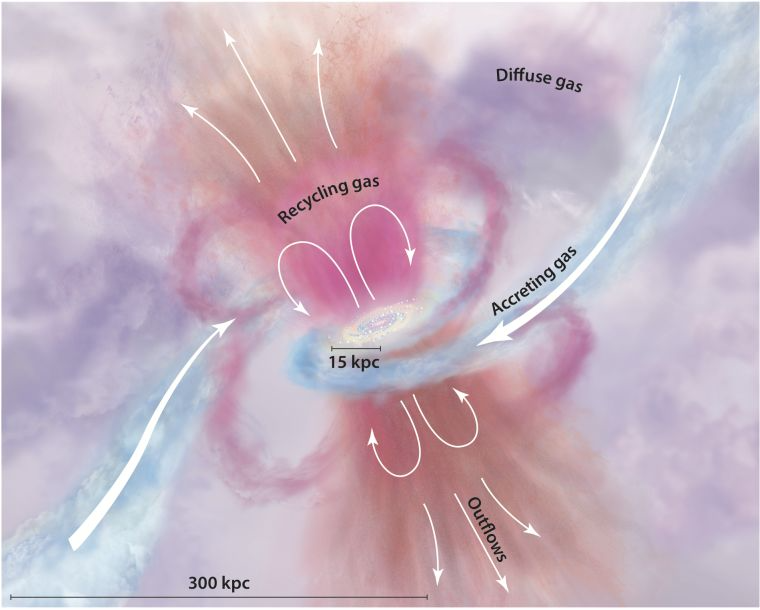
\includegraphics[scale=2.23]{Chapter-1/Figures/CGM_Tumlinson.png}
 \caption[Cartoon illustrating how material cycles through a star-forming galaxy and the circumgalactic medium (credit: J.\ Tumlinson)]{Cartoon illustrating how material cycles through a star-forming galaxy and the circumgalactic medium. Material from the intergalactic medium accretes onto the galaxy (shown in blue) while outflows (pink and orange) eject material out of the galaxy. Nearby bound material (pink) is largely recycled back to the galaxy while expelled material (orange) either contributes to large-scale accretion (blue) or exists as diffuse gas (purple). Image credit: Tumlinson, et al.~(2017) \cite{Tumlinson17}.}\label{fig:CGM_Tumlinson}
 \end{figure}
The scenario of galactic feedback just described is illustrated\footnote{Image credit is owed to J.\ Tumlinson \cite{Tumlinson17}.} in \cref{fig:CGM_Tumlinson}, which depicts a galaxy with a diameter of about \num{15} \emph{kiloparsecs} (kpc)\footnote{Defined as the distance associated with a parallax measurement of one arcsecond ($\SI{1}{\arcsecond} \equiv \SI{1}{\degree}/3600$), one \emph{parsec} (\num{1}~pc) is about \SI{3.086e16}{\metre} or equivalently, \num{3.262} light years. For comparison, the distance to the nearest star, Proxima Centauri, is $\sim \num{1.3}$~pc while the diameter of the Milky Way is $\gtrapprox 30$~kpc.} and the circumgalactic medium with a size scale of \num{300}~kpc. 
As shown in the figure, the galaxy expels material through outflows while circumgalactic and intergalactic media feed accretion back to the galactic disk. 

Soft x-ray spectroscopy fits into this picture of the \emph{cosmic baryon cycle} with its exclusive ability to diagnose highly-ionized portions of diffuse plasmas that are expected to constitute a significant fraction of the total baryon content in the Universe \cite{Persic92,Bregman07,McGaugh10}. 
That is, while measurements of elemental abundance ratios from primordial nucleosynthesis \cite{Kirkman03} and acoustic oscillations observed in the \emph{cosmic microwave background} \cite{Komatsu09,Planck_collab} indicate that baryons should constitute $\gtrapprox \SI{4}{\percent}$ of the total mass-energy contained in the low-redshift Universe, stellar and gaseous material contained within galaxies, groups and clusters accounts for only $\gtrapprox \SI{10}{\percent}$ \cite{Persic92,Fukugita_2004,Bregman07}. 
The remaining $\lessapprox \SI{90}{\percent}$ is thought to reside in the extended halos of isolated galaxies, groups or clusters,\footnote{Stated differently, this refers to the outer portions of circumgalactic, intragroup or intracluster media, where plasma density is sufficiently low so as to prevent direct detection. This is in contrast to the diffuse x-ray emission easily observed throughout the bulk of rich clusters \cite{Sarazin86}.} and additionally, the intergalactic medium, where extremely low plasma density (down to $\sim 1$ particle \si{\per\metre\cubed}) makes spectroscopic detection difficult and often times prohibitive due to instrumental limitations \cite{Fukugita_2004,Bregman07,Shull12}. 
Approximately half of this material that exists outside of isolated galaxies, groups and clusters is expected to comprise the \emph{warm-hot intergalactic medium}, where filamentary structures of the \emph{cosmic web} are heated to \SIrange{e5}{e7}{\kelvin} by collisionless shocks induced by galactic feedback and gravitational effects of large-scale structure formation \cite{Cen99,Dave01,Nicastro05b,Nicastro08,Bykov08,deGraaff19}. 
Measuring this diffuse, highly-ionized baryonic content through soft x-ray absorption spectroscopy along the line-of-sight of active galactic nuclei is a main scientific objective for the \emph{Lynx X-ray Observatory} \cite{Lynx_web} that can only be carried out using state-of-the-art grating spectroscopy. 
One of four flagship mission concepts considered for the 2020 Astrophysics Decadal Survey \cite{Gaskin19,Gaskin15}, \emph{Lynx}, if selected, will replace the spacecraft x-ray observatories \emph{Chandra} \cite{Weisskopf00} and \emph{XMM-Newton} \cite{Jansen01,Lumb12} that have provided large amounts of scientific return since their deployment to Earth's orbit in the late 1990s. 
The \emph{X-ray Grating Spectrometer (XGS)} currently being planned for \emph{Lynx} baselines next-generation instrumentation that provides substantial improvements over the transmission grating spectrometers on board \emph{Chandra} \cite{Canizares05,Brinkman00} and the \emph{Reflection Grating Spectrometer (RGS)} of \emph{XMM-Newton} \cite{Kahn96,denHerder01} in terms of both spectral resolving power and spectral sensitivity \cite{McEntaffer19,Gunther19}. 

Leveraging from the \emph{RGS}, one of two main designs considered for the \emph{XGS} uses arrays of specialized reflection gratings integrated into the \emph{Lynx} telescope assembly to produce a soft x-ray diffraction pattern that is imaged and order-separated by detectors at the focal plane so that spectra can be extracted \cite{McEntaffer19}. 
Achieving high spectral resolving power and high spectral sensitivity with this spectrometer requires thousands of custom, high-precision gratings that each perform with high diffraction efficiency to be carefully manufactured and aligned in modular arrays. %\footnote{Discussed in \cref{sec:measure_efficiency,ap:grating_basics}, this quantity can be understood as the relative brightness of each diffracted beam produced by an illuminated grating.}
Bearing this in mind, the focus of this dissertation is on a series of laboratory experiments that demonstrate the ability of two recently-developed nanofabrication techniques in the areas of electron-beam lithography and nanoimprint lithography, namely \emph{thermally-activated selective topography equilibration} and \emph{substrate-conformal imprint lithography}, to pattern gratings with sawtooth surface reliefs (\emph{i.e.}, \emph{blazed gratings}) that are appropriate for such an application, with an emphasis on characterizing their diffraction-efficiency performance through beamline testing \cite{McCoy16,McCoy17,McCoy18,McCoy20,McCoy20b}. 
To provide background and motivation for this work, which was largely carried out at the Penn State Materials Research Institute \cite{PSU_MRI} and the Advanced Light Source at Lawrence-Berkeley National Laboratory \cite{ALS_web,LBNL_web}, this chapter first describes why sensitive, high-resolution grating spectroscopy is indispensable for measuring weak absorption lines in the soft x-ray that are produced as continuum emission from an active galactic nucleus passes through diffuse, intergalactic plasmas.  %circumgalactic and intergalactic media. 
Specifications for x-ray reflection gratings and previously-established methodology for their fabrication are then presented before the chapter concludes with an outline of this thesis document. %measuring weak absorption lines at soft x-ray wavelengths
This chapter builds on physics background outlined in \cref{ap:x-ray_intro,ap:quantum_spectral,app:x-ray_materials,ap:grating_basics} while SI units and the fundamental constants listed in \cref{tab:units,tab:fundamental_constants} are used throughout this dissertation.\footnote{I reserve credit for all micrographs, images and figures unless noted otherwise.} 

\section{Soft X-ray Spectroscopy of Highly-Charged Ions in Extended Galactic Halos and the Intergalactic Medium}\label{sec:astro_plasmas}
%%%%%%%%%%%%%%%%%%%%%%%%%%%%%%%%%%%%%%%%%-------------------------------------------------- 
In principle, highly-charged ions in extended halos of isolated galaxies, groups, or clusters, and the warm-hot intergalactic medium are observable spectroscopically as a given ionic species undergoes a bound-bound electronic transition that results in the emission or absorption of photons with energy centered around the difference in electronic binding energies, $\Delta \mathcal{E}_e$ [\emph{cf.\@} \cref{ap:quantum_spectral}]. 
A naturally-broadened spectral line takes the form of a \emph{Lorentzian distribution} [\emph{cf.\@} \cref{eq:normalized_lorentzian_QM}], which is written as a function of photon energy, $\mathcal{E}_{\gamma}$, as 
\begin{equation}\label{eq:Lorentzian_1} 
 \phi_{\text{nat}} \left( \mathcal{E}_{\gamma} , \Gamma \right) = \frac{1}{2 \pi} \left( \frac{\hbar^2 \Gamma}{\left(\mathcal{E}_{\gamma} - \Delta \mathcal{E}_e \right)^2 + \frac{\hbar^2}{4} \Gamma^2} \right) ,
 \end{equation}
where $\hbar$ is the reduced Planck's constant and $\Gamma$ is the quantum-mechanical transition rate derived in \cref{sec:transition_rate_sub}, which is equivalent to the relevant \emph{Einstein coefficient} for the process \cite{Rybicki86}. 
Spectral lines associated with bound-bound transitions occur at soft x-ray photon energies only in highly-charged ions that have ionization potentials, $\chi$, on the order of hundreds of \si{\electronvolt}, which is characteristic of an electron temperature, $T_e$, on the order of $\chi / k_{\mathcal{B}} \sim \SI{e6}{\kelvin}$, where $k_{\mathcal{B}}$ is the Boltzmann constant. 
With electrons and ions equilibrated in a plasma, $T_e$ is equal to the temperature of a particular species of ion, $T_{\text{ion}}$, and hence the effect of thermal broadening is expected to be significant for these spectral lines. 
\begin{figure}
 \centering
 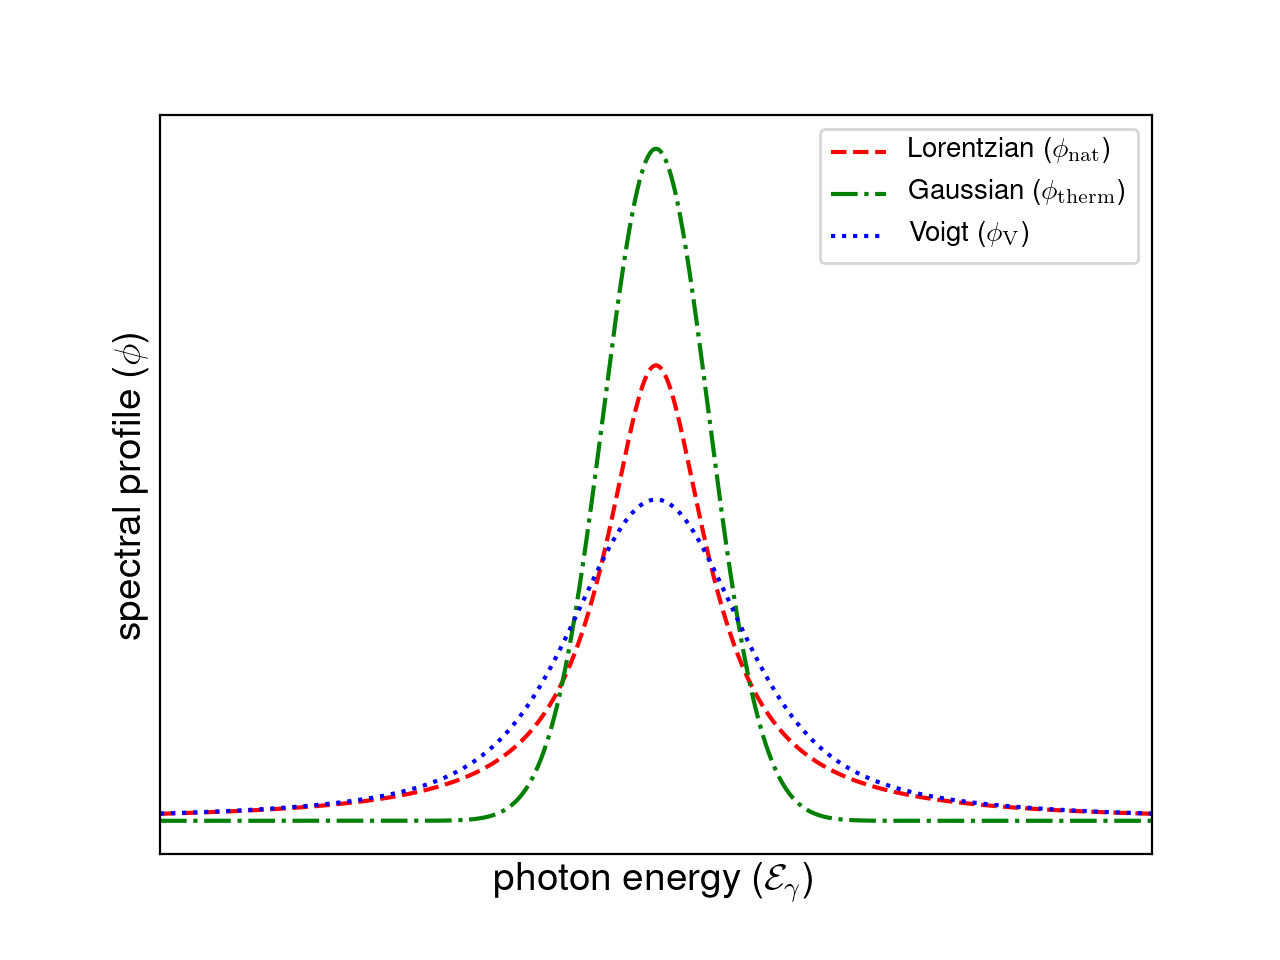
\includegraphics[scale=1]{Chapter-1/Figures/spectral_lines.png}
 \caption[Spectral lines as a function of photon energy for Lorentzian, Gaussian and Voigt profiles.]{Spectral lines as a function of photon energy, $\mathcal{E}_{\gamma}$, for Lorentzian, Gaussian and Voigt profiles [\emph{cf.\@} \cref{eq:Lorentzian_1,eq:normalized_thermal_QM,eq:voigt}] with line centroids corresponding to $\mathcal{E}_{\gamma} = \Delta \mathcal{E}_e$, the electronic binding energy difference associated with the relevant bound-bound transition. The width of the Lorentzian profile describes natural broadening and depends on the quantum-mechanical transition rate, $\Gamma$ [\emph{cf.\@} \cref{sec:transition_rate_sub}], while the width of the Gaussian profile depends on the degree of thermal motion in the plasma, which is characterized by the quantity $\Delta \mathcal{E}_D$ [\emph{cf.\@} \cref{eq:Doppler_width}]. Neglecting collisional broadening, the Voigt profile is the convolution of these two functions, which then depends on both $\Gamma$ and $\Delta \mathcal{E}_D$.}\label{fig:spectral_lines}
 \end{figure}
This contribution to a spectral line profile takes the form of a \emph{Gaussian distribution}:
\begin{subequations}
\begin{equation}\label{eq:normalized_thermal_QM}
 \phi_{\text{therm}} \left( \mathcal{E}_{\gamma} , \Delta \mathcal{E}_D \right) \equiv \frac{1}{\Delta \mathcal{E}_D \sqrt{2 \pi}} \mathrm{e}^{-\left( \mathcal{E}_{\gamma} - \Delta \mathcal{E}_e \right)^2 / 2 \Delta \mathcal{E}_D^2} ,
 \end{equation}
where 
\begin{equation}\label{eq:Doppler_width}
 \Delta \mathcal{E}_D \equiv \Delta \mathcal{E}_e \sqrt{\frac{2 k_{\mathcal{B}} T_{\text{ion}}}{m_{\text{ion}} c_0^2}} %see pg 288 of R&L for derivation
 \end{equation} 
is the \emph{Doppler width} of the ions with $m_{\text{ion}}$ as the ion mass [\emph{cf.\@} \cref{tab:astro_element_nuclei_mass}] and $c_0$ as the speed of light \cite{Rybicki86}. 
\end{subequations}
Due to the extremely low densities characteristic of the plasmas considered, the effect of collisional broadening can be neglected and thus an overall \emph{Voigt profile} that combines \cref{eq:Lorentzian_1,eq:normalized_thermal_QM} can be written as the convolution of the functions $\phi_{\text{nat}} \left( \mathcal{E}_{\gamma} , \Gamma \right)$ and $\phi_{\text{therm}} \left( \mathcal{E}_{\gamma} , \Delta \mathcal{E}_D \right)$:
\begin{equation}\label{eq:voigt}
 \phi_{\text{V}} \left( \mathcal{E}_{\gamma}, \Gamma, \Delta \mathcal{E}_D \right) \equiv \int_{-\infty}^{\infty} \phi_{\text{therm}} \left( \mathcal{E}_{\gamma} , \Delta \mathcal{E}_D \right) \, \phi_{\text{nat}} \left( \mathcal{E}_{\gamma} - \mathcal{E}'_{\gamma} , \Gamma \right) \dd{\mathcal{E}'_{\gamma}},
 \end{equation}
which describes the shape of a general spectral line from a hot, diffuse plasma. %the theoretical shape
These three spectral profiles are compared in \cref{fig:spectral_lines}, where it is seen that \cref{eq:Lorentzian_1,eq:normalized_thermal_QM} convolve to yield a Voigt profile with a Gaussian-like core and Lorentzian-like wings. 

Discussed in \cref{ap:quantum_spectral}, the most abundant species of highly-charged ions that exist at $\sim \SI{e6}{\kelvin}$ temperatures are \emph{hydrogen-like} and \emph{helium-like} ions of low-to-mid $\mathcal{Z}$, where just one or two bound electrons remain, respectively. 
The strongest x-ray spectral lines from such ions are expected to be those associated with \emph{electric-dipole transitions}, also known as \emph{resonance lines}, that occur between the K-shell and L-shell [\emph{cf.\@} \cref{sec:multipole}; \cref{tab:astro_element_lyman_approx,tab:astro_element_he_res}]. 
Other x-ray spectral lines, such as those arising from \emph{intercombination} and \emph{forbidden} transitions in helium-like ions [\emph{cf.\@} \cref{tab:astro_element_he_interx,tab:astro_element_he_intery,tab:astro_element_he_forb}] meanwhile are relatively dim but play an important role in plasma diagnostics of emitting sources \cite{Porquet2010,Paerels03,Kahn02}. 
In extended galactic halos and the intergalactic medium, radiative transitions in highly-charged ions are driven by collisional excitement due to there being a lack of a strong x-ray source illuminating the plasma. 
This can be described using the \emph{principle of detailed balance} for a hypothetical two-level atom in a collisional plasma with an electronic binding energy difference $\Delta \mathcal{E}_e$ between two bound states:
\begin{equation}
 n_1 n_e C_{12} = n_2 n_e C_{21} + n_2 A_{21} ,
 \end{equation}
which relates the Einstein coefficients that describe transition rates for collisional excitement, $C_{12}$, to those for collisional de-excitement, $C_{21}$, and \emph{spontaneous emission},\footnote{The principle of spontaneous emission, where a photon is emitted as an excited atomic electron transitions to its ground state, is described using quantum mechanics of photons and non-relativistic bound electrons in \cref{sec:single_absorption_emission}.} $A_{21}$, where $n_e$ is the number density of energetic free electrons in the plasma while $n_1$ and $n_2$ are the number densities of bound electrons in the ground state and the excited state, respectively \cite{Mo10}. 

The average time in between collisions for a very diffuse plasma is much longer than the timescales associated with radiative decay in highly-charged ions, which are remarkably short due to the transition rate of such a transition, $\Gamma = A_{21}$, depending on $\Delta \mathcal{E}_e^2$ as described in \cref{sec:transition_rate_sub}. 
Thus, with collisional de-excitement neglected and excitations depending on two-body collisions between electrons and ions with volume densities $n_e$ and $n_{\text{ion}}$, respectively, the overall intensity of emission lines is then expected to be proportional to the \emph{emission measure} of the plasma, defined as 
\begin{equation}\label{eq:emission_measure}
 \text{EM} = \int n_e n_{\text{ion}} \dd[3]{\mathbold{r}} ,
 \end{equation}
where the integration is carried out over the volume of the emitting plasma \cite{Paerels03}. 
While x-ray grating spectroscopy is best suited for point sources as argued in \cref{sec:grating_tech_dev}, energy-dispersive detectors that are able to gather spectra of extended sources can measure emission lines from these diffuse plasmas in areas where $\text{EM}$ [\emph{cf.\@} \cref{eq:emission_measure}] is sufficiently large, such as in the bulk of intracluster media \cite{Bohringer10}. 
However, emission spectroscopy of highly-charged ions in extremely low-$n_e$ plasmas, such as those present in extended galactic halos and the intergalactic medium, demands levels of sensitivity that far surpass the capabilities the capabilities of state-of-the-art instruments of this type, such as the currently-planned \emph{Lynx Microcalorimeter (LXM)} \cite{Bandler19}. %that far surpass the capabilities
To circumvent this issue, x-ray absorption spectroscopy using active galactic nuclei as background sources must be employed, and as motivated in the following discussion, highly-efficient grating spectrometers capable of high spectral resolving power are required to detect faint absorption lines that characterize plasma density among other physical parameters. 

\subsection{Weak Absorption Lines From Active Galactic Nuclei}\label{sec:weak_absorb}
%%%%%%%%%%%%%%%%%%%%%%%%%%%%%%%%%%%%%%%%%--------------------------------------------------
An \emph{active galactic nucleus} describes a system where there exists an accretion disk around the galaxy's supermassive black hole, along with a hot corona and a surrounding torus of neutral gas and dust \cite{Schneider06,Carroll07,Mo10,Netzer13}. 
Associated with such a system are jets aligned with the axis of rotation and ionized winds emanating from the accretion disk; this scenario is illustrated\footnote{Image credit is owed to A.\ Simonnet (\url{http://auroresimonnet.com/}).} in \cref{fig:agn_cartoon}. 
%that are thought to populate circumgalactic and intergalactic media with baryonic matter. 
\begin{figure}
 \centering
 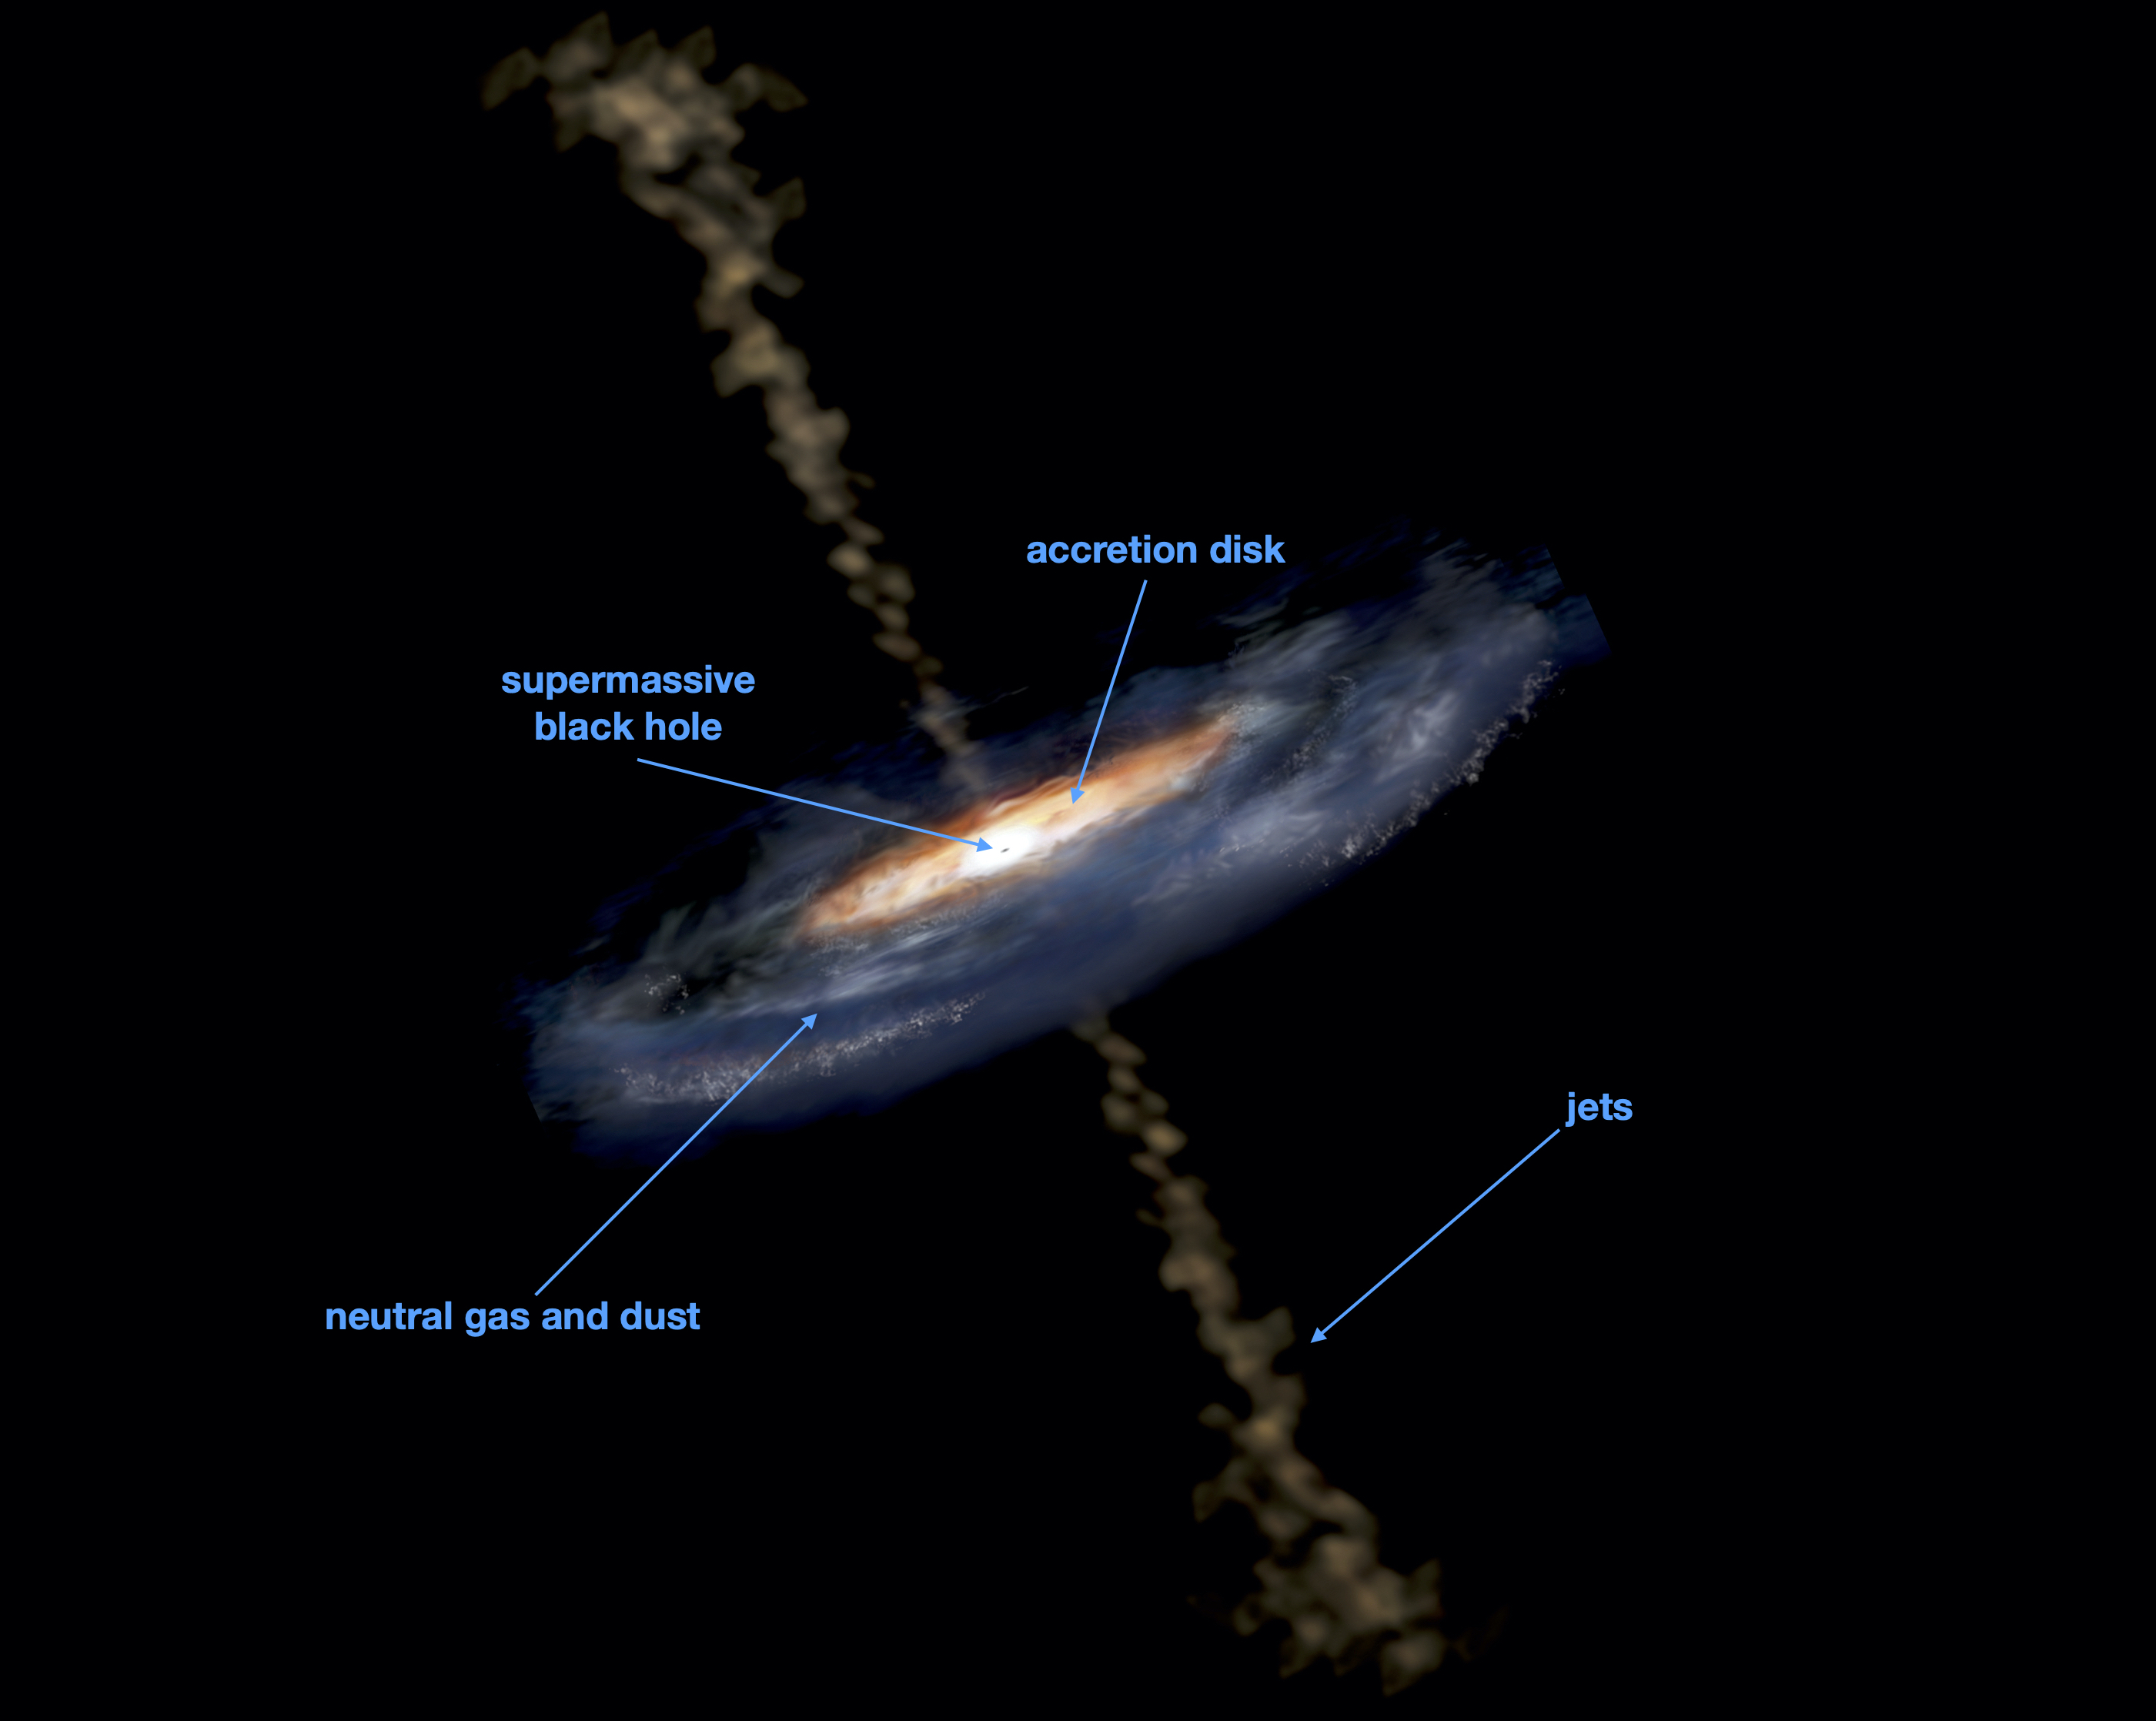
\includegraphics[scale=0.15]{Chapter-1/Figures/agn_big_edit.jpg}
 \caption[Cartoon of an active galactic nucleus (credit: A.\ Simmonnet)]{Cartoon of an active galactic nucleus. An accretion disk surrounds the immediate vicinity of the central supermassive black hole while further out radially, there exists a torus of neutral gas and dust. Moreover, a hot corona and ionizing winds (not shown) surround the inner accretion disk while jets of material are aligned with its axis of rotation. Image credit: A.\ Simonnet.}\label{fig:agn_cartoon}
 \end{figure}
In principle, the temperature of the accretion disk, $T$, is a decreasing function of radius, $r$, with $T \propto r^{-3/4}$ that typically maximizes around \SI{e5}{\kelvin} \cite{Schneider06}. 
The power radiated through a surface of unit area as a function of photon energy, $\mathcal{E}_{\gamma}$, produced by a single annulus of temperature $T$ is characteristic of a \emph{black-body radiator} described by \emph{Planck's law} \cite{Carroll07,Rybicki86}:
\begin{subequations}
\begin{equation}\label{eq:Planck_law}
 B (\mathcal{E}_{\gamma}, T) = \frac{\mathcal{E}_{\gamma}^3}{2 \pi^2 \hbar^2 c_0^2} \frac{1}{ \mathrm{e}^{\mathcal{E}_{\gamma} / k_{\mathcal{B}} T} - 1} ,
 \end{equation}
while according to \emph{Wein's displacement law}: 
\begin{equation}\label{eq:Wein_law}
 \lambda_{\text{max}} = \frac{b}{T} \quad \text{with } b = \SI{2.897771955e-3}{\meter\kelvin} ,
 \end{equation} 
\end{subequations}
the wavelength of radiation associated with a typical maximum temperature of $T \sim \SI{e5}{\kelvin}$, $\lambda_{\text{max}}$, falls in the far ultraviolet (UV). 
Taking into account the entire accretion disk with $T \propto r^{-3/4}$, the resulting UV continuum spectrum is a summation of blackbody spectra that manifests as a power law spectrum \cite{Schneider06}. 

X-rays are produced indirectly by such an accretion disk predominantly through the \emph{inverse Compton effect}, where highly-energetic electrons transfer momentum to the optical and UV photons generated by blackbody radiation \cite{Haardt91,Schneider06,Netzer13}. 
%Although the accretion disk itself is not a strong source of x-rays by the above argument, active galactic nuclei are indeed bright x-ray sources. 
%Active galactic nuclei typically are bright x-ray sources notwithstanding that the accretion disk itself is not a strong source of x-rays by the above argument. 
%This is thought to be because the corona is responsible for up-scattering UV photons produced by the accretion disk into x-rays through the \emph{inverse Compton effect}, where highly-energetic electrons transfer momentum to photons; 
While the result is also a continuum spectrum that appears as a power law, soft x-ray emission measured from active galactic nuclei typically exceeds extrapolations from higher $\mathcal{E}_{\gamma}$; this is the so-called \emph{soft x-ray excess}, which has several proposed emission mechanisms \cite{Walter93,Schneider06,Crummy06,Gliozzi20}. %, often taken as $\mathcal{E}_{\gamma}^{-0.7}$,
In cases where the jets of an active galactic nucleus are oriented toward Earth, the object is viewed as a \emph{blazar} with bright, beamed emission produced from \emph{synchrotron radiation}, which also manifests as a power law for a distribution of electron energies \cite{Rybicki86,Schneider06,Netzer13,Pal20}. %\cite{Pal20}
Active galactic nuclei thus are suitable background sources for absorption spectroscopy of highly-charged ions in extended galactic halos and the intergalactic medium, with blazars being desirable due to their particularly high x-ray brightness.\footnote{Another class of x-ray sources are \emph{x-ray binaries}: binary star systems where one of the stars exists as a compact object such as a neutron star or a black hole, which accretes material from the other. However, these x-ray sources are typically a few orders of magnitude dimmer than active galactic nuclei \cite{Schneider06}.}  %, and moreover, their intensity is often unstable over relatively short timescales

As described in \cref{sec:form_spectral}, an absorption line is formed as a particular species of ion along the line-of-site of a continuum source absorbs a narrow spectral distribution of soft x-rays centered around $\mathcal{E}_{\gamma} = \Delta \mathcal{E}_e$, the electronic binding energy difference associated with a bound-bound transition from the ground state to some excited bound state. 
The \emph{spectral flux}, $\mathcal{F}$,\footnote{This quantity is defined as radiative intensity per unit area, per unit time, per photon energy \cite{Rybicki86}.} absorbed by such a transition, in principle, takes the form of $\phi_{\text{V}} \left( \mathcal{E}_{\gamma}, \Gamma, \Delta \mathcal{E}_D \right)$ [\emph{cf.\@} \cref{eq:voigt}] with fixed values for $\Gamma$ and $\Delta \mathcal{E}_D$. 
The spectral flux of the absorption line, $\mathcal{F}_{\text{line}}$, then is the difference between the background continuum spectral flux, here taken as $\mathcal{F}_c \propto \mathcal{E}_{\gamma}^{-0.7}$, and this Voigt profile [\emph{cf.\@} \cref{fig:absorption_line}]. 
\begin{figure}
 \centering 
 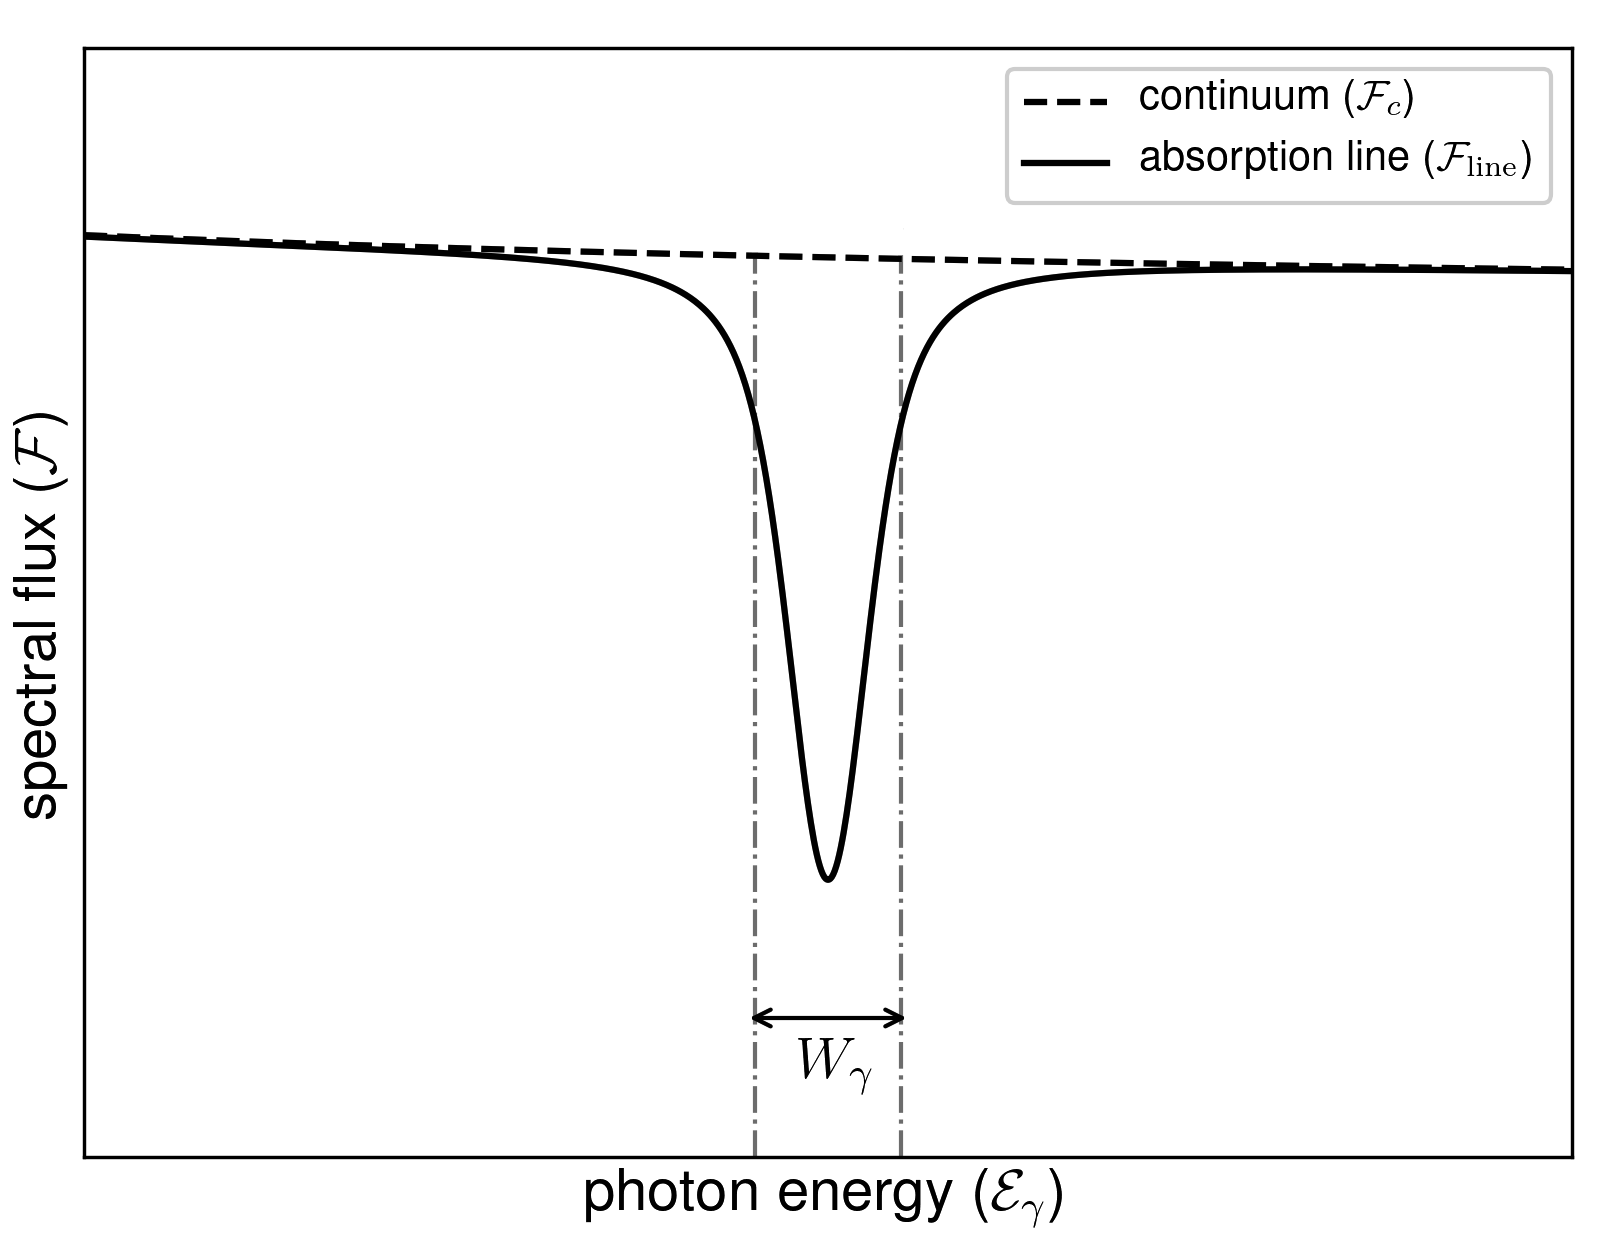
\includegraphics[scale=0.245]{Chapter-1/Figures/equiv.png}%absorption_line.png}
 \caption[Spectral flux of an absorption line as a function of photon energy]{Spectral flux of an absorption line as a function of photon energy, $\mathcal{F}_{\text{line}}$, where the line centroid corresponds to $\mathcal{E}_{\gamma} = \Delta \mathcal{E}_e$. By construction, $\mathcal{F}_{\text{line}}$ is the difference between the underlying continuum spectral flux, $\mathcal{F}_c \propto \mathcal{E}_{\gamma}^{-0.7}$, and a spectral profile associated with the absorption line, which is assumed to take the form of a Voigt profile [\emph{cf.\@} \cref{eq:voigt}].}\label{fig:absorption_line}
 \end{figure}
Depending on the \emph{optical depth} of a given species of highly-charged ion in the absorbing plasma, the strength of such an absorption line can be quantified using an \emph{equivalent width} \cite{Carroll07}, defined in terms of photon energy as 
%The strength of such an absorption line, which depends on the \emph{optical depth} of a given species of highly-charged ion in the absorbing plasma, can be quantified using an \emph{equivalent width} defined in terms of photon energy as 
\begin{equation}\label{eq:EW_gen}
 W_{\gamma} \equiv \int \left(  \frac{\mathcal{F}_c - \mathcal{F}_{\text{line}}}{\mathcal{F}_c} \right) \dd{\mathcal{E}_{\gamma}} = \int \left(  1 - \mathrm{e}^{- \tau^{\text{ion}}_{\gamma}} \right) \dd{\mathcal{E}_{\gamma}}  ,
 \end{equation} 
where, for a given absorbing ion, $\tau^{\text{ion}}_{\gamma} \equiv \sigma^{\text{ion}}_{\gamma} \mathcal{N}^{\text{ion}}_{\gamma}$ is the optical depth per photon energy, $\sigma^{\text{ion}}_{\gamma}$ is the cross-section per photon energy for absorption, which depends on $\Gamma$ for the relevant bound-bound absorption process [\emph{cf.\@} \cref{sec:transition_rate_sub}] and $\mathcal{N}^{\text{ion}}_{\gamma}$ is the column density per photon energy, defined as 
\begin{equation}
 \mathcal{N}^{\text{ion}}_{\gamma} = \int n^{\text{ion}}_{\gamma} \dd{\ell} , 
 \end{equation}
where $n^{\text{ion}}_{\gamma}$ is the volume density of ions absorbing at a photon energy $\mathcal{E}_{\gamma}$ and the integral over $\ell$ represents the line-of-sight of the observation \cite{Carroll07}.  
In diffuse plasmas of extended galactic halos and the intergalactic medium, $\mathcal{N}^{\text{ion}}_{\gamma}$ is very small and hence it is justified to make the approximation $\mathrm{e}^{-\tau^{\text{ion}}_{\gamma}} \approx 1 - \tau^{\text{ion}}_{\gamma}$ so that %the quantity $\mathcal{N}^{\text{ion}}_{\gamma}$ is very small
\begin{equation}\label{eq:EW_od_thin}
 W_{\gamma} \approx \int \tau^{\text{ion}}_{\gamma} \dd{\mathcal{E}_{\gamma}}
 \end{equation} 
and from comparing \cref{eq:EW_gen} and \cref{eq:EW_od_thin}, 
\begin{equation}
 \tau^{\text{ion}}_{\gamma} \approx \frac{\mathcal{F}_c - \mathcal{F}_{\text{line}}}{\mathcal{F}_c} .
 \end{equation}
Therefore, a measurement for $W_{\gamma}$ of a weak absorption line directly yields the optical depth for a specific highly-charged ion, and through $\mathcal{N}^{\text{ion}}_{\gamma} = \tau^{\text{ion}}_{\gamma} / \sigma^{\text{ion}}_{\gamma}$, the density of a given ionic species present in the plasma can be inferred. 

The overall function of an energy-dispersive spectrometer such as the \emph{LXM} is to bin collected photons by their energy, $\mathcal{E}_{\gamma}$, into spectral intervals of width $\Delta \mathcal{E}_{\gamma}$ so that the instrument's spectral resolving power, $\mathscr{R} = \mathcal{E}_{\gamma} / \Delta \mathcal{E}_{\gamma}$, by definition indicates its ability to distinguish between photons with $\mathcal{E}_{\gamma}$ and $\mathcal{E}_{\gamma} + \Delta \mathcal{E}_{\gamma}$ in the process of measuring a spectrum. 
Unresolved, weak absorption lines can be measured within a single resolution bin, $\Delta \mathcal{E}_{\gamma}$, and in this case \cref{eq:EW_gen} becomes\footnote{The following analysis regarding equivalent widths and a figure of merit for spectral line detection is based on an unpublished document written by J.\ Kaastra for the \emph{International X-ray Observatory} mission concept in 2008 \cite{McEntaffer09,McEntaffer10}.} 
\begin{equation}\label{eq:EW_int}
 W_{\gamma} = \left( \frac{\mathcal{F}_c - \mathcal{F}_{\text{line}}}{\mathcal{F}_c} \right) \Delta \mathcal{E}_{\gamma} \equiv \frac{F_{\text{line}}}{\mathcal{F}_c} \approx \tau^{\text{ion}}_{\gamma} \Delta \mathcal{E}_{\gamma} ,
 \end{equation}
where $F_{\text{line}} \equiv \left[ \mathcal{F}_c - \mathcal{F}_{\text{line}} \right] \Delta \mathcal{E}_{\gamma} = \mathcal{F}_c W_{\gamma}$ is the flux missing from the continuum due to the absorption line within the spectral interval $\Delta \mathcal{E}_{\gamma}$. 
Owing to their high $\mathcal{E}_{\gamma}$ and low count rates in astronomy, x-rays are practically measured as individual particles that obey \emph{Poisson statistics}, which dictate that the probability for the number of photons detected during an observation is given by 
\begin{equation}\label{eq:poisson}
 \mathscr{P} \left( N=N_{\text{tot}} \right) = \mathrm{e}^{-N_{\text{tot}}} \frac{N^N_{\text{tot}}}{N!} ,
 \end{equation}
where $N_{\text{tot}}$ is the average number of photons collected during a given observation time, $t_{\text{obs}}$, with $\sqrt{N_{\text{tot}}}$ as the standard deviation describing \emph{shot noise} \cite{siemiginowska_2011,Sturge03}. 
In the case of absorption spectroscopy, $N_{\text{tot}}$ is essentially the number of photons absorbed by the plasma subtracted from the number of continuum photons. 
The number of photons associated with the absorption line that are detected with an instrumental collecting area $A_{\text{col}}$ and an exposure time $t_{\text{obs}}$ is 
\begin{subequations}
\begin{equation}\label{eq:line_count}
 N_{\text{line}} \equiv F_{\text{line}} A_{\text{col}} t_{\text{obs}} 
 \end{equation}
while, using $A_{\text{col}} t_{\text{obs}} = N_{\text{line}} / F_{\text{line}}$ [\emph{cf.\@} \cref{eq:line_count}] and $W_{\gamma} = F_{\text{line}} / \mathcal{F}_c$ [\emph{cf.\@} \cref{eq:EW_int}], the number of photons from the continuum detected across the spectral interval $\Delta \mathcal{E}_{\gamma}$ is 
\begin{equation}\label{eq:cont_count}
 N_c \equiv \mathcal{F}_c \Delta \mathcal{E}_{\gamma} A_{\text{col}} t_{\text{obs}} = N_{\text{line}} \frac{\Delta \mathcal{E}_{\gamma}}{W_{\gamma}} .
 \end{equation}
 The total number of counts detected from a spectral line within an interval $\Delta \mathcal{E}_{\gamma}$, neglecting instrumental background,\footnote{In principle, such a background due to dark current, for example, contributes to this total through $N_b \equiv \mathcal{F}_b \Delta \mathcal{E}_{\gamma} A_{\text{col}} t_{\text{obs}}$, where $\mathcal{F}_b$ is the spectral flux associated with the signal.} then is
\begin{equation}\label{eq:total_count}
 N_{\text{tot}} \equiv N_c - N_{\text{line}} = N_{\text{line}} \left( \frac{\Delta \mathcal{E}_{\gamma}}{W_{\gamma}} - 1 \right) = N_c \left( 1 - \frac{W_{\gamma}}{\Delta \mathcal{E}_{\gamma}} \right) , 
 \end{equation}
\end{subequations}
with the corresponding counting error being approximately $\sqrt{N_c}$ for weak spectral lines with $\abs{W_{\gamma}} \ll \Delta \mathcal{E}_{\gamma}$. 

Detecting an absorption line with statistical significance hinges on having a sufficiently large \emph{signal-to-noise ratio}: 
\begin{equation}\label{eq:signal_noise}
 \mathcal{S} \equiv \frac{N_{\text{line}}}{\sqrt{N_{\text{tot}}}} = \sqrt{\frac{N_{\text{line}}}{\frac{\Delta \mathcal{E}_{\gamma}}{W_{\gamma}} - 1}} , 
 \end{equation}
where $N_{\text{line}}$, the number of photons absorbed by the spectral line, is the signal and $\sqrt{N_{\text{tot}}}$ is the shot noise [\emph{cf.\@} \cref{eq:poisson}]. 
With $N_{\text{line}} = N_c \left( W_{\gamma} / \Delta \mathcal{E}_{\gamma} \right)$ [\emph{cf.\@} \cref{eq:cont_count}] inserted into \cref{eq:signal_noise}, the minimum number of photons associated with the continuum that must be detected to achieve a signal-to-noise ratio $\mathcal{S}_0$ is described by the following inequality: 
\begin{equation}
 N_c > \mathcal{S}_0^2 \left( \frac{\Delta \mathcal{E}_{\gamma}}{W_{\gamma}} - 1 \right) \left( \frac{\Delta \mathcal{E}_{\gamma}}{W_{\gamma}} \right) \approx \left( \frac{\Delta \mathcal{E}_{\gamma}}{W_{\gamma}} \right)^2 \mathcal{S}_0^2 , 
 \end{equation}
which indicates that having a small resolution bin, $\Delta \mathcal{E}_{\gamma}$, or high $\mathscr{R} = \mathcal{E}_{\gamma} / \Delta \mathcal{E}_{\gamma}$, is needed for distinguishing weak absorption lines from dim continua. 
As $N_{\text{line}}$ [\emph{cf.\@} \cref{eq:line_count}] depends on the flux absorbed by the spectral line, $F_{\text{line}}$, the observation exposure time, $t_{\text{obs}}$, and the collecting area of the instrument, $A_{\text{col}}$, the only quantity that is inherent to a specific instrument is the latter, $A_{\text{col}}$. 
An appropriate figure of merit (FOM) for an instrument's ability to detect a spectral line then should be proportional to $\mathcal{S}$ [\emph{cf.\@} \cref{eq:signal_noise}], but without the dependence on $F_{\text{line}}$ and $t_{\text{obs}}$ for a specific observation: 
\begin{subequations}
\begin{equation}\label{eq:FOM}
 \text{FOM} \propto \frac{\mathcal{S}}{\sqrt{F_{\text{line}} t_{\text{obs}}}} = \frac{\sqrt{A_{\text{col}}}}{\sqrt{\frac{\Delta \mathcal{E}_{\gamma}}{W_{\gamma}} - 1}} .
 \end{equation}
Provided that they can be resolved, relatively strong spectral lines with $\abs{W_{\gamma}} \gg \Delta \mathcal{E}_{\gamma}$ have $\text{FOM} \propto \sqrt{A_{\text{col}}}$ and hence line detection depends on collecting area alone. 
On the other hand, for weak absorption lines with $\abs{W_{\gamma}} \ll \Delta \mathcal{E}_{\gamma}$, \cref{eq:FOM} reduces to 
\begin{equation}\label{eq:FOM_weak}
 \text{FOM}_{\text{weak}} \propto \frac{\mathcal{S}}{\sqrt{F_{\text{line}} t_{\text{obs}}}} \approx \sqrt{\frac{A_{\text{col}} W_{\gamma}}{\Delta \mathcal{E}_{\gamma}}} \propto \sqrt{A_{\text{col}} \mathscr{R}} ,
 \end{equation}
\end{subequations}
which shows that the detection of such a line has the same dependence on both instrument collecting area and spectral resolving power. %, $\mathscr{R} = \mathcal{E}_{\gamma} / \Delta \mathcal{E}_{\gamma}$. 
This latter relation can be rearranged to give 
\begin{equation}
 t_{\text{obs}} \propto \frac{\mathcal{S}^2}{\text{FOM}_{\text{weak}}^2 F_{\text{line}}} \propto \frac{1}{A_{\text{col}} \mathscr{R}} ,
 \end{equation}
which indicates that making improvements in instrument collecting area and spectral resolving power both serve to reduce the observation time required to achieve a signal-to-noise ratio $\mathcal{S}$ in a weak absorption line. 

\subsection{The Need for Next-Generation X-ray Gratings}\label{sec:need_gratings}
%%%%%%%%%%%%%%%%%%%%%%%%%%%%%%%%%%%%%%%%%--------------------------------------------------
The performance of a grating spectrometer differs fundamentally from an energy-dispersive instrument in that radiation is binned according to wavelength, $\lambda$, so that its wavelength-dispersive spectral resolving power, $\mathscr{R} = \lambda / \Delta \lambda$, indicates its ability to distinguish between radiation with $\lambda$ and $\lambda + \Delta \lambda$ in the process of measuring a spectrum [\emph{cf.\@} \cref{ap:grating_basics}]. 
This can be seen to be beneficial for soft x-ray absorption spectroscopy by noting that the spectral resolving power of an energy-dispersive instrument, $\mathscr{R} = \mathcal{E}_{\gamma} / \Delta \mathcal{E}_{\gamma}$, improves as $\mathcal{E}_{\gamma}$ increases and degrades as $\mathcal{E}_{\gamma}$ decreases.\footnote{That is, provided the resolution bin size, $\Delta \mathcal{E}_{\gamma}$, stays roughly constant across a given bandpass.} 
With the opposite being true for wavelength-dispersive instruments, where $\mathscr{R} = \lambda / \Delta \lambda$, a grating spectrometer with sufficiently small $\Delta \lambda$ lends itself to the detection of weak absorption lines with $\mathcal{E}_{\gamma} \lessapprox \SI{1}{\kilo\electronvolt}$, where the equivalent width in terms of wavelength, $W_{\lambda}$, is related to $W_{\gamma}$ [\emph{cf.\@} \cref{eq:EW_gen}] through 
\begin{equation}
 \frac{W_{\lambda}}{\lambda} = \frac{W_{\gamma}}{\mathcal{E}_{\gamma}} \implies W_{\lambda} = \frac{\lambda^2}{h c_0} W_{\gamma} = \frac{2 \pi h c_0}{\mathcal{E}^2_{\gamma}} W_{\gamma} 
 \end{equation}
with $h \equiv 2 \pi \hbar$ and $h c_0 \approx \SI{1240}{\electronvolt\nm}$. 
On the other hand, energy-dispersive instruments are beneficial for higher-energy spectral lines such as those associated with highly-charged ions of iron [\emph{cf.\@} \cref{tab:astro_element_lyman_approx,tab:astro_element_he_res}] and additionally, relatively bright emission lines from extended sources such as supernova remnants \cite{Dewey10,Ballet02}. 

As oxygen is the most abundant element beyond hydrogen and helium, hydrogen-like and helium-like charge states of this atom (\emph{i.e.}, \ion{O}{viii} and \ion{O}{vii}, respectively), with prominent absorption lines centered at $\mathcal{E}_{\gamma}^{\text{\ion{O}{viii}}} \approx \SI{653.4}{\electronvolt}$ and $\mathcal{E}_{\gamma}^{\text{\ion{O}{vii}}} \approx \SI{574.0}{\electronvolt}$, are the most important contributors for x-ray absorption studies of diffuse plasmas in extended galactic halos and the intergalactic medium. %circumgalactic and intergalactic media. 
Along with analogous spectral lines from highly-charged ions of other relatively abundant elements such as carbon, neon and nitrogen [\emph{cf.\@} \cref{tab:astro_element_lyman_approx,tab:astro_element_he_res}] these absorption lines moreover are generally Doppler shifted, predominantly by \emph{cosmological redshift}, $z$, which serves to decrease the measured photon energy, $\mathcal{E}'_{\gamma}$ \cite{Liddle03,Carroll07}: 
\begin{equation}\label{eq:energy_shift}
 \frac{\mathcal{E}_{\gamma}}{\mathcal{E}'_{\gamma}} \equiv 1 + z \implies \mathcal{E}'_{\gamma} = \frac{\mathcal{E}_{\gamma}}{1+z}.
 \end{equation}
Although a small number of absorbing \ion{O}{vii} systems associated with the warm-hot intergalactic medium have been claimed through statistical analyses of data gathered by the grating spectrometers of \emph{XMM-Newton} and \emph{Chandra} with stacked observing times, $t_{\text{obs}}$, on the order of \si{\mega\second} \cite{Nicastro18,Kovacs19}, a spectrometer with a large $\text{FOM}_{\text{weak}} \propto \sqrt{A_{\text{col}} \mathscr{R}}$ for $\mathcal{E}_{\gamma} \lessapprox \SI{1}{\kilo\electronvolt}$ is needed for detecting weak absorption lines in these diffuse plasmas with higher statistical confidence and reducing the required $t_{\text{obs}}$. 
Explicitly, with $\Delta \mathcal{E}_{\gamma} = \SI{3}{\electronvolt}$ and $A_{\text{col}} \approx \SI{1000}{\cm\squared}$ baselined for the main component of the \emph{LXM}, $\mathscr{R}$ is on the order of a few hundred for $\mathcal{E}_{\gamma} \lessapprox \SI{1}{\kilo\electronvolt}$. 
While this yields an improvement over the \emph{RGS} on board \emph{XMM-Newton} in terms of $\text{FOM}_{\text{weak}}$, which also exhibits $\mathscr{R}$ of a few hundred but with $A_{\text{col}} \approx \SI{150}{\cm\squared}$, both $\mathscr{R}$ and $A_{\text{col}}$ still must be increased to make significant improvements to $\text{FOM}_{\text{weak}}$ and hence \textbf{a next-generation grating spectrometer is required for the detection of weak absorption lines in extended galactic halos and the intergalactic medium}. 

A point of reference for $\mathscr{R}$ is the spectral resolving power associated with a thermally-broadened oxygen line: 
\begin{equation}
 \mathscr{R}_D \equiv \frac{\mathcal{E}_{\gamma}}{\Delta \mathcal{E}_D} = \frac{\mathcal{E}_{\gamma}}{\Delta \mathcal{E}_e} \sqrt{\frac{m_{\text{ion}} c_0^2}{2 k_{\mathcal{B}} T_{\text{ion}}}} \gtrapprox 5000 , 
 \end{equation}
where the Doppler width, $\Delta \mathcal{E}_D$, is given by \cref{eq:Doppler_width} using $T_{\text{ion}} \lessapprox \SI{e7}{\kelvin}$ as a typical ion temperature and $m_{\text{ion}} = \SI{2.656e-26}{\kilogram}$ as the mass of an oxygen-16 nucleus [\emph{cf.\@} \cref{tab:astro_element_nuclei_mass}]. 
The \emph{XGS} for \emph{Lynx} aims to achieve this spectral resolving power by maintaining $\Delta \lambda = \abs{n} \lambda / \mathscr{R}_D \lessapprox \SI{0.4}{\pico\metre} = \SI{4}{\milli\angstrom}$ across the soft x-ray bandpass using order numbers $n =$ \numrange{5}{8} for blazed reflection gratings \cite{McEntaffer19} or higher orders using \emph{critical-angle transmission gratings} \cite{Gunther19}. 
Additionally, the instrument baselines $A_{\text{col}} \gtrapprox \SI{4000}{\cm\squared}$ for spectral sensitivity, which requires gratings that perform with $\gtrapprox \SI{40}{\percent}$ \emph{total absolute diffraction efficiency}\footnote{This refers to the sum of absolute diffraction efficiency in all propagating orders with order number $n \neq 0$ [\emph{cf.\@} \cref{sec:grating_tech_intro,sec:measure_efficiency}].} at soft x-ray wavelengths. 
In principle, these specifications are achievable using x-ray reflection grating technology, which is the subject of \cref{sec:grating_tech_dev}. 

With a large $\text{FOM}_{\text{weak}}$ baselined for the \emph{XGS}, this instrument planned for \emph{Lynx} will be able to measure equivalent widths of soft x-ray absorption lines much smaller than what is possible with the \emph{LXM} as well as the grating spectrometers on board \emph{XMM-Newton Newton} or \emph{Chandra}. 
Additionally, a spectral resolving power of $\mathscr{R}_D \gtrapprox 5000$ enables the velocities of ionized outflows that emanate from active galactic nuclei to be measured with precision on the order of tens of \si{\kilo\metre\per\second}. 
This can be seen by noting that the definition of redshift [\emph{cf.\@} \cref{eq:energy_shift}] gives
\begin{subequations}
\begin{equation}\label{eq:wave_shift}
 \frac{\lambda'}{\lambda} \equiv 1 + z \implies z = \frac{\overbrace{\lambda'-\lambda}^{\Delta \lambda}}{\lambda} = \frac{1}{\mathscr{R}}
 \end{equation}
while for a velocity $v \ll c_0$, 
\begin{equation}
 \frac{v}{c_0} = \frac{\left( 1 + z \right)^2 - 1}{\left( 1 + z \right)^2 + 1} \approx z 
 \end{equation}
\end{subequations}
so that the smallest velocity resolved is $v = c_0 / \mathscr{R}_D \lessapprox c_0 / 5000$. 
By design, the \emph{XGS} is expected to be capable of measuring $W_{\lambda}$ for absorption lines on the level of $\SI{0.1}{\pico\metre} = \SI{1}{\milli\angstrom}$ while the \emph{RGS} of \emph{XMM-Newton} is typically used to measure $W_{\lambda}$ on the order of several \si{\pico\metre}, or tens of \si{\milli\angstrom}. 
\emph{Lynx} observation strategies for studies of intergalactic soft x-ray absorption sample plasmas along the line-of-sight of a large number of active galactic nuclei at various cosmological redshifts, $z$. 

As the most prominent soft x-ray absorption lines, the resonance lines from hydrogen-like and helium-like oxygen with rest-frame wavelength centroids $\lambda_{\text{\ion{O}{viii}}} \approx \SI{1.90}{\nm}$ and $\lambda_{\text{\ion{O}{vii}}} \approx \SI{2.16}{\nm}$, respectively, practically place a limit on these values for $z$. 
\begin{figure}
 \centering
 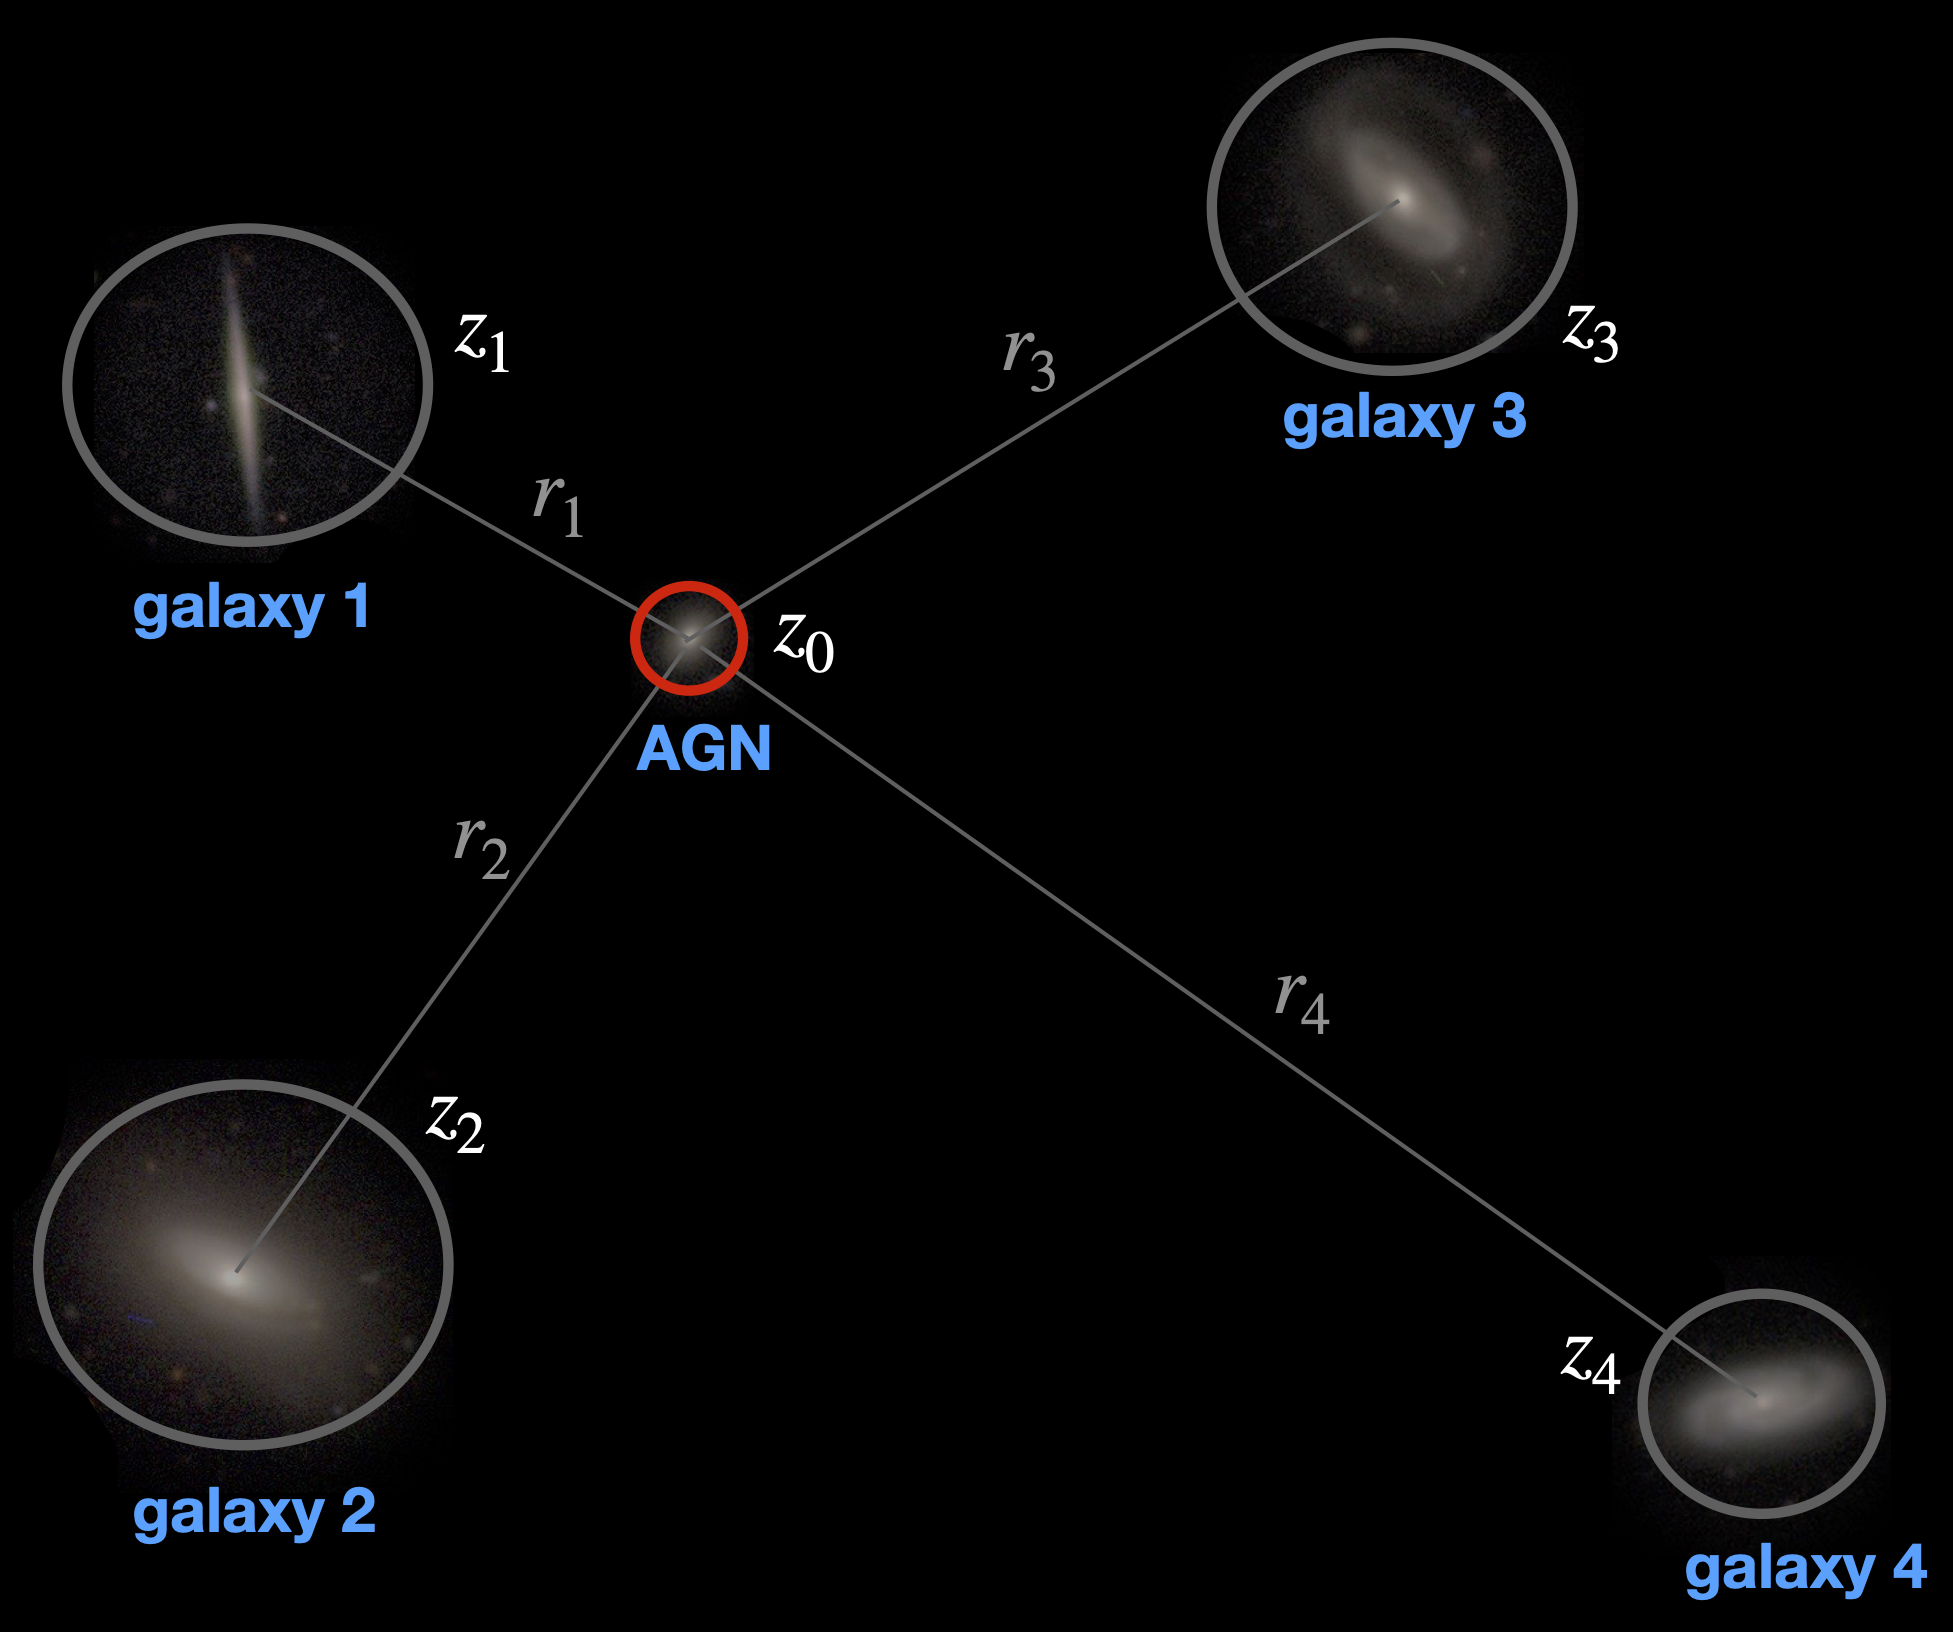
\includegraphics[scale=0.45]{Chapter-1/Figures/galaxy_field.png} 
 \caption[Cartoon of an active galactic nucleus with four galaxies in the foreground for absorption spectroscopy]{Cartoon of an active galactic nucleus (AGN) at a redshift $z_0$ with four isolated galaxies at smaller redshifts $z_i$ (for $i=$ \numrange{1}{4}) in the foreground. In principle, a spectroscopic observation of the AGN with sufficiently large $\text{FOM}_{\text{weak}} \propto \sqrt{A_{\text{col}} \mathscr{R}}$ [\emph{cf.\@} \cref{eq:FOM_weak}] probes the density of highly-charged ions present in extended galactic halos and intergalactic medium at radial distances $r_i$ (for $i=$ \numrange{1}{4}) from the nuclear region of each galaxy. The result is a spectrum featuring prominent absorption lines from each intervening galaxy with centroids that depend on $z_i$ and equivalent widths that give an indication of plasma density, which in turn depends on $r_i$. The depicted galaxies are optical images obtained from \textsc{Galaxy Zoo}.}\label{fig:galaxy_field}
 \end{figure}
That is, using $\lambda' = (1 + z) \lambda$ [\emph{cf.\@} \cref{eq:wave_shift}] and noting that the red end of the soft x-ray exists at $\lambda \approx \SI{6}{\nm}$, \ion{O}{vii} and \ion{O}{viii} resonance lines are observable out to $z \approx 1.6$ and $z \approx 2$, respectively, where the Universe is observed \numrange{5}{10} billion years in the past. 
Illustrated\footnote{The galaxies depicted in \cref{fig:galaxy_field} are images obtained from \textsc{Galaxy Zoo} \cite{galaxy_zoo,Lintott08} but in this context, they are not intended to represent specific objects on the celestial sphere.} in \cref{fig:galaxy_field}, x-ray continuum emission from a distant active galactic nucleus with relatively high $z$ will generally be absorbed by highly-charged ions in the intergalactic medium and, if the line-of-sight passes near galaxies of lower $z$, circumgalactic, intragroup or intraculster media. 
Thus, by measuring $W_{\lambda}$ for many absorbing systems and correlating their measured redshift with that of intercepting galaxies, the density of extragalactic baryons can effectively be probed as a function of distance from a galactic nucleus and additionally, across cosmic time. 
Overall, these observations serve to track the highly-ionized portion of baryons that cycle through galaxies and are a prime example of a scientific objective that can only be accomplished with a next-generation grating spectrometer. 


\section{Development of X-ray Reflection Gratings}\label{sec:grating_tech_dev}
%%%%%%%%%%%%%%%%%%%%%%%%%%%%%%%%%%%%%%%%%--------------------------------------------------
Making spectral observations in the soft x-ray, like in any spectral bandpass, requires channeling radiation according to its \emph{color} and then measuring the relative intensity of each component present to extract a spectrum. 
For UV and other electromagnetic radiation with $\lambda \gtrapprox \SI{100}{\nm}$, this is commonly carried out with wavelength-dispersive instruments in telescopes that utilize diffraction gratings \cite{Loewen97,Ryden10}. 
While x-rays are often measured spectroscopically as energetic particles, the soft x-ray bandpass has $\lambda$ ranging from several \si{\nm} down to about \SI{0.5}{\nm}, where diffraction gratings can be used to obtain sensitive, high-resolution spectra if implemented appropriately. 
Although this has been achieved with the grating spectrometers on board spacecraft observatories \emph{XMM-Newton} \cite{Jansen01,denHerder01,Lumb12} and \emph{Chandra} \cite{Canizares00,Weisskopf00}, these instruments face throughput limitations that result in poor signal-to-noise for distinguishing faint absorption lines from background continua [\emph{cf.\@} \cref{sec:astro_plasmas}]. 
With future x-ray observatories such as \emph{Lynx} \cite{Gaskin19,Lynx_web} calling for improvements in spectral sensitivity and spectral resolving power, $\mathscr{R} = \lambda / \Delta \lambda$, across the soft x-ray bandpass, this section motivates the investigation of new ways to produce highly-efficient reflection gratings with custom groove layouts that are capable of addressing these technological challenges. 

\subsection{General Grating-Design Considerations}\label{sec:grating_tech_intro}
%%%%%%%%%%%%%%%%%%%%%%%%%%%%%%%%%%%%%%%%%--------------------------------------------------
To introduce specifications for reflection gratings that push the state of the art for x-ray spectroscopy, it is useful to consider how an x-ray reflection grating spectrometer compares and contrasts with more conventional grating spectrometers used for astronomical spectroscopy at longer wavelengths. 
For example, in a common reflecting telescope designed for visible light, focusing mirrors are used at near-normal incidence and typically several reflections can occur without significant loss in throughput. 
This enables the implementation of an \emph{echelle spectrometer}, where light passes through an entrance pinhole or slit before being re-focused by various secondary optics so that collimated light is incident on a planar reflection grating with steep, triangular groove facets ruled uniformly over a relatively coarse groove spacing, $d$ \cite{Ryden10,Loewen97}. 
As described in \cref{sec:slit_array}, a low $\lambda / d$ ratio yields a large number of propagating orders while according to the scalar treatment of diffraction efficiency outlined in \cref{sec:sawtooth_principle}, far-field intensity is maximized in the direction of the diffracted angle $\beta = 2 \delta - \alpha$, where $\alpha$ is the incidence angle and $\delta$ is the \emph{blaze angle}, which characterizes the slope of the sawtooth facets. 
Thus, for such an \emph{echelle grating} with large $\delta$, diffraction efficiency is concentrated into high orders on one side of $0^{\text{th}}$ order, which in turn leads to high $\mathscr{R}$, with throughput maximized in a specified bandpass that depends on $\delta$ and $d$ \cite{Loewen97}. 
The result is a set of overlapping spectra, one for each propagating order, that are separated through the use of a second diffraction grating or other dispersive instrument (\emph{e.g.}, a prism) before they are imaged by a detector as an \emph{echellogram} \cite{Ryden10}. 
The extracted spectra in such a situation are often diffraction limited and hence require an echelle grating with a large grooved area to attain high $\mathscr{R}$ [\emph{cf.\@} \cref{sec:resolving_power}]. %  as described in \cref{sec:resolving_power}. 

In a somewhat similar vein to an echelle spectrometer, a traditional x-ray reflection grating spectrometer utilizes focusing mirrors and blazed gratings to disperse radiation collected by the telescope into spectra that are ultimately imaged by a detector at the focal plane. 
However, there are substantial differences that have their roots in the fact that significant x-ray reflection from an optical surface can only be achieved at grazing-incidence angles in the regime of \emph{total external reflection} [\emph{cf.\@} \cref{sec:planar_interface}]. %, which is described from first principles in \cref{sec:planar_interface}. 
With this restriction of grazing incidence, any single mirror or reflection grating appears small in projection to incident radiation; therefore, many nested mirrors and gratings, each with a substantial size, must be stacked and aligned into modules to achieve a sufficient collecting area for spectroscopy, $A_{\text{col}}$ \cite{Cash91,Kahn96,Allured13,Allured15,Donovan18,Shipley08,McEntaffer11}. 
Grazing-incidence focusing in an x-ray telescope is commonly achieved using the \emph{Wolter-I} design \cite{Wolter52}, where nested parabolic mirror segments begin to focus collimated light from an astronomical source before the focal length is reduced significantly by a following set of hyperbolic mirror segments that bring radiation to a focus several meters away \cite{Aschenbach85,schwartz_2011}. 
The fundamental difficulties of x-ray reflection [\emph{cf.\@} \cref{app:x-ray_materials}] combined with the fact that astrophysical spectral signatures of interest in the soft x-ray are quite faint\footnote{\emph{e.g.}, weak absorption lines from extended galactic halos and the intergalactic medium [\emph{cf.\@} \cref{sec:astro_plasmas}]} lead to a practical inability to re-collimate radiation collected by the telescope before it is incident on a grating. 
As an alternative strategy, modular grating arrays can be positioned to intercept the radiation coming to a focus in the telescope while an imaging detector placed at the focal plane is used to record the dispersed spectrum. %spectra?
In this case, order separation is carried out not by a secondary grating or prism as in a typical echelle spectrometer, but rather by the energy-dispersive response of the imaging detector, so that further reflections are not necessary \cite{Cash91}. 
Moreover, without an entrance slit or pinhole, the entire image collected by the Wolter-I optics passes through the spectrometer and as a result, high-resolution spectroscopy with such an instrument is functionally limited to point sources \cite{schwartz_2011}. 
The \emph{RGS} on board \emph{XMM-Newton} is the first space-borne instrument to realize this concept, where \num{182} identical gratings aligned into modular arrays intercept the radiation being focused by Wolter-I optics consisting of \num{58} nested mirror pairs while \emph{charge-coupled device} detectors are used to image the diffraction pattern and to carry out order separation \cite{Kahn96,denHerder01}. 

There exist two classes of grazing-incidence grating geometries that have been pursued for astronomical x-ray spectroscopy. 
This can be gleaned from noting the location of the $n^{\text{th}}$ order diffracting from a grating with a groove spacing $d$ at an arbitrary, oblique incidence angle, which is described by the \emph{generalized grating equation} \cite[\emph{cf.\@} \cref{eq:off-plane_incidence_orders}]{Loewen97}: 
\begin{equation}\label{eq:off-plane_orders}
 \sin \left( \alpha \right) + \sin \left( \beta \right) = \frac{n \lambda}{d \sin \left( \gamma \right)} \quad \text{for } n = 0, \pm 1, \pm 2, \pm 3 \dotsc 
 \end{equation}
As illustrated in the left panel of \cref{fig:conical_reflection_edit} and explained further in \cref{sec:off-plane_geo}, $\gamma$ is the half-opening angle of the cone, $\alpha$ is the azimuthal incidence angle and $\beta$ is the azimuthal diffracted angle of the $n^{\text{th}}$ diffracted order. 
\begin{figure}
 \centering
 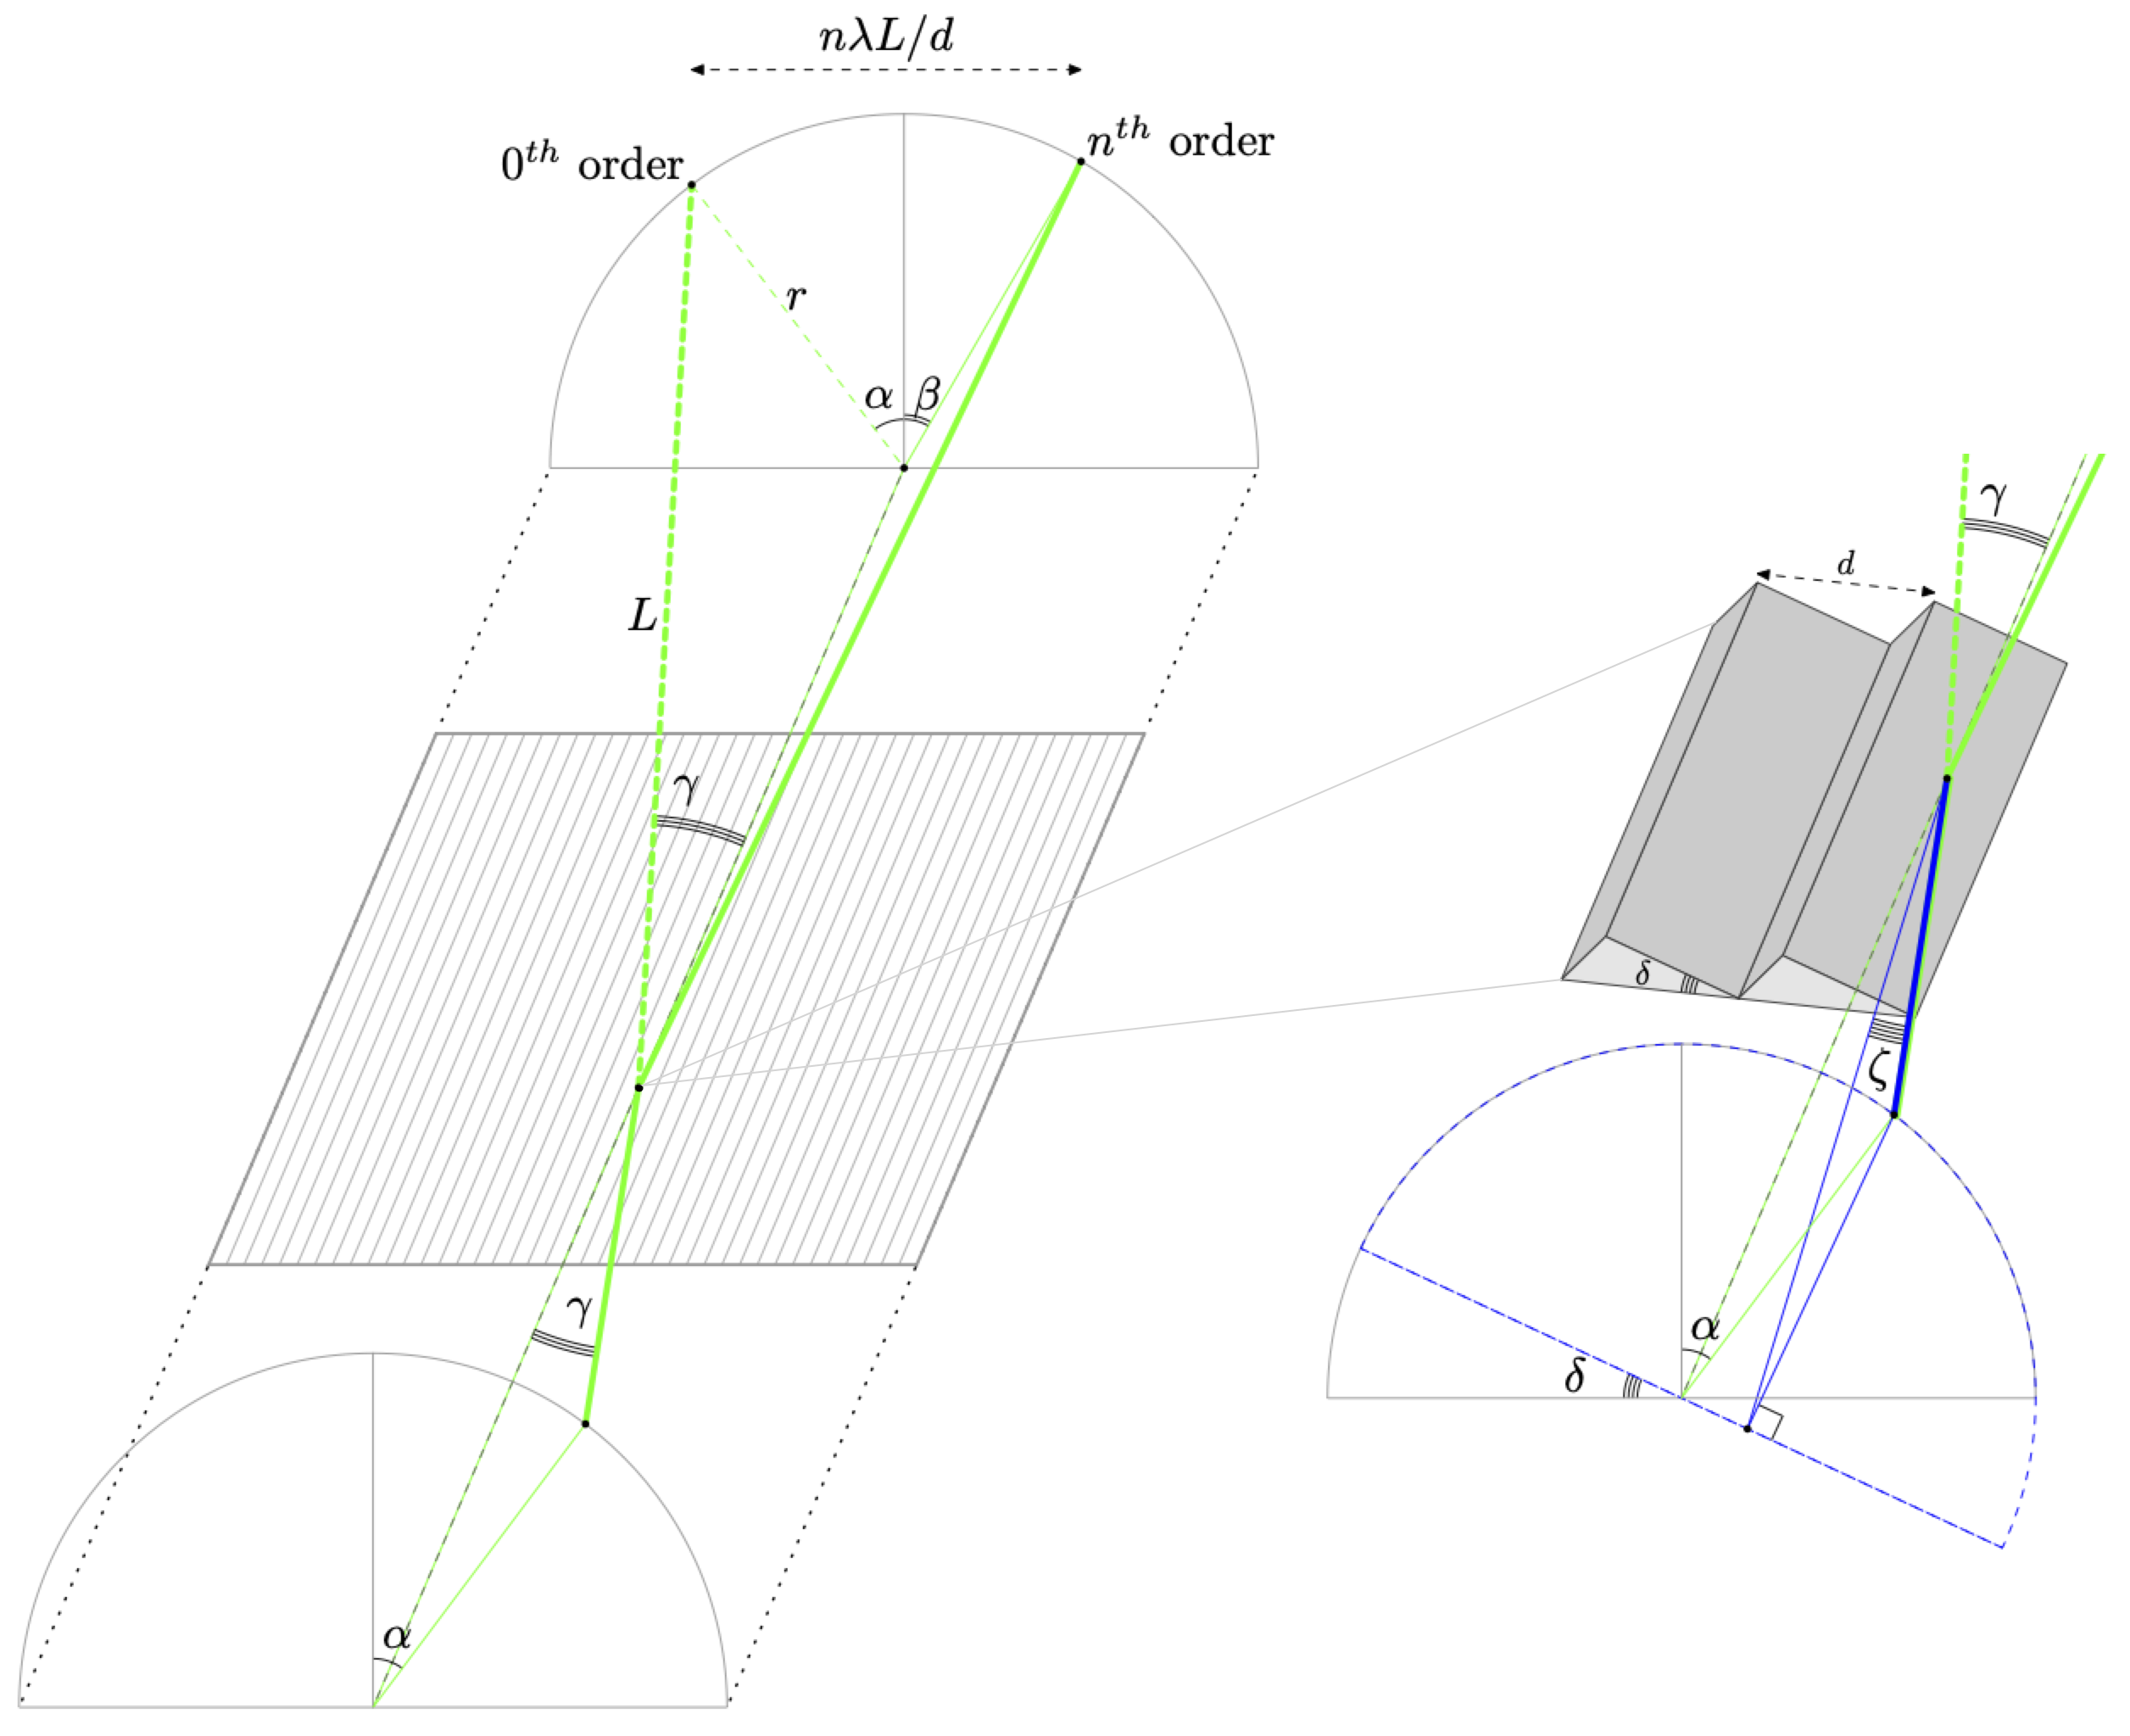
\includegraphics[scale=0.165]{Chapter-1/Figures/grat_geo_fix2.png}
 \caption[Reflection grating geometry for conical diffraction.]{Reflection grating geometry for conical diffraction. In an extreme off-plane mount, the incoming radiation is nearly parallel to the groove direction such that the half-angle of the cone opening, $\gamma$, is on the order of a degree. Because of this, the angle on the groove facets, $\zeta$, is a grazing-incidence angle for any value of $\alpha$ that illuminates the shallow side of the sawtooth profile with a blaze angle $\delta$. At a distance $L$ away from the point of incidence on the grating, diffracted orders are each separated by a distance $\lambda L / d$ along the direction of grating periodicity (\emph{i.e.}, the grating-dispersion direction), where $d$ is the groove spacing \cite{McCoy18,McCoy20}.}\label{fig:conical_reflection_edit}
 \end{figure} 
At a distance $L$ from the point of incidence on the grating (\emph{i.e.}, the \emph{throw} of the system), each propagating order with $n \neq 0$ is dispersed along the cross-groove direction by a distance from $0^{\text{th}}$ order given by
\begin{equation}\label{eq:linear_dispersion}
 x_n = \frac{n \lambda L}{d} 
 \end{equation}
and confined along the arc of a circle with a radius given by
\begin{equation}\label{eq:arc_radius}
 r = L \sin \left( \gamma \right) .
 \end{equation}
Radiation is incident on the sawtooth facets of a blazed grating at an angle $\zeta$ as illustrated in the right panel of \cref{fig:conical_reflection_edit}, which is related to $\alpha$ and $\gamma$ through the following relation:
\begin{equation}\label{eq:angle_on_groove}
 \sin \left( \zeta \right) = \sin \left( \gamma \right) \cos \left( \delta - \alpha \right) .
 \end{equation} 
Assuming that only the shallow side of the asymmetric, sawtooth-shaped grooves is illuminated, the result, in principle, is that radiation is preferentially diffracted to an angle $\beta = 2 \delta - \alpha$, so that for each propagating order coinciding with this angle, diffraction efficiency is maximized at the \emph{blaze wavelength}, which is given for the $n^{\text{th}}$ diffracted order by \cref{eq:blaze_wavelength_general}:
\begin{subequations}
\begin{equation}\label{eq:blaze_wavelength}
 \lambda_b = \frac{d \sin \left( \gamma \right)}{n} \left[ \sin \left( \alpha \right) + \sin \left( 2 \delta - \alpha \right) \right] .
 \end{equation}
Therefore, to take into account the grazing-incidence requirement that $\zeta$ be a small angle on the groove facets, commonly one of two grating geometries is employed:
\begin{enumerate}[noitemsep]
  \item A grazing-incidence, \emph{in-plane} geometry, where $\sin \left( \gamma \right) = 1$ such that incoming radiation is perpendicular to the groove direction and \cref{eq:angle_on_groove} yields $\zeta = \pi/2 - \alpha + \delta$, necessitating $\alpha$ approaching $90^{\circ}$ and a very shallow $\delta$ 
  \item An extreme \emph{off-plane} geometry, where $\gamma \lessapprox 2^{\circ}$ so that by \cref{eq:angle_on_groove}, $\zeta$ is always small and hence $\alpha$ is free to match $\delta$ in a projected \emph{Littrow configuration} \cite{Loewen97}, where $\alpha = \beta = \delta$ and $\zeta = \gamma$ 
\end{enumerate}
In the former case, a shallow blaze angle leads to diffraction efficiency being maximized in low order and moreover, higher orders with smaller $\beta$ are often vignetted in tightly-packed grating arrays. 
The latter case, on the other hand, allows for high efficiency in high order with appropriate choice of $\delta$, which in turn leads to high $\mathscr{R}$ in a bandpass of interest \cite{Werner77,Cash82,Cash91}. 
This is commonly achieved in a Littrow configuration, where $\alpha = \beta = \delta$ and \cref{eq:blaze_wavelength} reduces to \cref{eq:blaze_wavelength_Litt} \cite{Neviere78b}:
\begin{equation}\label{eq:blaze_wavelength_Littrow}
 \lambda_b = \frac{2 d \sin \left( \gamma \right) \sin \left( \delta \right)}{n} .
 \end{equation}
\end{subequations}
Additionally, an extreme off-plane geometry enables tight packing geometries for modular arrays without vignetting losses thanks to a small cone-opening angle, $2 \gamma$ \cite{Cash91}. 
While the \emph{RGS} on board \emph{XMM-Newton} was designed using a grazing-incidence, in-plane grating geometry, it is for these reasons that much of the recent and current instrument development for future observatories considers the extreme off-plane geometry to make advances in $\mathscr{R}$ and spectral sensitivity \cite{McEntaffer03,McEntaffer04,McEntaffer08b,McEntaffer09,McEntaffer10,McEntaffer11,McEntaffer13,DeRoo16thesis,DeRoo16,Tutt16,Miles18,Donovan18,Miles19,DeRoo20a,Donovan20}. 

Regardless of the geometry employed, reflection gratings in a Wolter-I telescope are used in a converging beam of radiation and this necessitates a \emph{variable-line-space} groove layout that matches the focal length of the telescope to reduce, or potentially eliminate, grating-induced aberrations in the resulting spectrum \cite{Hettrick83}. 
In such a scenario, $\mathscr{R}$ is limited not by the number of grating grooves as is often the case for an echelle spectrometer [\emph{cf.\@} \cref{sec:resolving_power}], but rather by the preservation of the \emph{point spread function} generated by the primary mirrors of the Wolter-I telescope as the converging radiation is diffracted by non-uniform grating grooves. 
With an in-plane geometry employed for the \emph{RGS}, the variable-line-space profile on each grating features parallel grooves that have a gradually decreasing spacing toward the telescope focus with an average of $d \approx \SI{1.5}{\um}$ \cite{Kahn96,denHerder01}. 
This gradient in $d$ serves to counteract the non-negligible change in $L$ that rays pick up as they strike different parts of the grating at grazing incidence in order for a constant linear dispersion [\emph{cf.\@} \cref{eq:linear_dispersion}] to be maintained. 
Meanwhile, each grating is positioned such that radiation is incident on the grating perpendicular to the groove direction and as a result, there is no need for non-parallel grooves. 

On the other hand, the variable-line-space equivalent for an extreme off-plane geometry manifests as a \emph{radial groove profile}, where each groove points toward the telescope focus in a fanned groove pattern \cite{Cash83}. 
This groove layout creates a gradient in $d$ across the grating similar to the in-plane case, but additionally, the tilted grooves in principle ensure that $\alpha$ is constant across each grating in a converging beam of radiation. 
However, the extreme off-plane geometries utilized for soft x-ray spectroscopy typically require $d$ on the order of a few hundred \si{\nm} or less in a Littrow configuration for a moderate blaze angle (\emph{e.g.}, $\delta \approx 30^{\circ}$) while in most cases, $d$ can be larger for grazing-incidence, in-plane geometries with very shallow blaze angles. 
Discussed further in \cref{sec:off-plane_geo}, this can be gleaned from \cref{eq:off-plane_orders}, which reduces to \cref{eq:normal_incidence_orders} for an in-plane geometry: 
\begin{subequations}
\begin{equation}\label{eq:in-plane_orders_ch1}
 \sin \left( \alpha \right) + \sin \left( \beta \right) = \frac{n \lambda}{d} \quad \text{for } n = 0, \pm 1, \pm 2, \pm 3 \dotsc ,
 \end{equation}
where both $\alpha$ and $\beta = 2 \delta - \alpha$ are large for grazing-incidence diffraction, but with opposite signs, so that for small $\delta$ and $\alpha \lessapprox 90^{\circ}$, \cref{eq:in-plane_orders_ch1} can be written approximately as 
\begin{equation}\label{eq:inplane_limit}
 2 \delta \left( \frac{\pi}{2} - \alpha \right) \approx \frac{n \lambda}{d} \quad \text{for } n = 0, \pm 1, \pm 2, \pm 3 \dotsc ,
 \end{equation}
\end{subequations}
which indicates $d \gg \lambda$ for small $\abs{n}$. 
In contrast, a grazing-incidence, off-plane geometry with small $\gamma$ and $\alpha = \beta = \delta$ has \cref{eq:off-plane_orders} approximated as 
\begin{equation}\label{eq:offplane_limit}
 2 \gamma \sin \left( \delta \right) \approx \frac{n \lambda}{d} \quad \text{for } n = 0, \pm 1, \pm 2, \pm 3 \dotsc ,
 \end{equation}
which shows that $d$ is still much larger than $\lambda$, but by a smaller margin for moderate values of $\delta$. 

The demand for variable-line-space profiles that match specific telescope focal lengths (to enable high $\mathscr{R}$) combined with the need to control $d$ and $\delta$ (to maximize diffraction efficiency near $\lambda_b$ for each order) has the consequence that \textbf{custom diffraction gratings are needed for x-ray spectroscopy}. 
The gratings used for the \emph{RGS} are gold-coated replicas of a master grating fabricated by \emph{mechanical ruling engine}, where a sculpted diamond tip burnishes one groove at a time into a layer of soft metal coated on a substrate \cite{Kahn96,denHerder01}. 
With heritage dating back to the early $19^{\text{th}}$ century \cite{Fraunhofer1823,Compton25}, the mechanical ruling process gives rise to a sawtooth-like topography, where the effective blaze angle, $\delta$, depends directly on the shape of ruling tip. 
Owing to the development of mechanical ruling engines with interferometric feedback control \cite{Harrison49,Harrison55}, nanoscale groove placement precision is possible \cite{Loewen97}. 
However, while many gratings used for near-visible wavelengths are also commonly fabricated by mechanical ruling, gratings generally are not custom-made for specific instruments due to the high cost and difficulties\footnote{In particular, environmental stabilities and tip wear must be kept under control over the course of the days, weeks or months of ruling time that may be required for gratings with relatively large areas.} associated with the ruling process; instead, spectrometers are often designed around standardized gratings provided by manufacturers. 
Additionally, surface-topography constraints are imposed by the shape of the ruling tip and hence commercial gratings are commonly ruled only with certain blaze angles, groove spacings and sizes \cite{Loewen97}. 
With specifications for radially-ruled, off-plane gratings departing significantly from standard gratings fabricated by mechanical ruling engine, realizing such an idealized groove profile for gratings with relatively large areas and controllable blaze angles requires identifying appropriate fabrication processes suitable for generating custom groove architectures that can be replicated to produce a large number of gratings. 
This motivates the investigation of techniques in the area of nanofabrication to produce new reflection gratings that each perform with high diffraction efficiency while maintaining an ability to realize a custom, variable-line-space profile that matches the focal length of a specific Wolter-I telescope. 

\subsection{Grating Fabrication}\label{sec:grating_fab_intro}
%%%%%%%%%%%%%%%%%%%%%%%%%%%%%%%%%%%%%%%%%--------------------------------------------------
Fabrication methods for x-ray reflection gratings have evolved significantly since the 1990s, when the gratings for the \emph{RGS} were manufactured by mechanical ruling engine and a replication process that involves casting replicas in a synthetic resin \cite{Kahn96,denHerder01}. 
This subsection outlines the main efforts for fabricating x-ray reflection gratings and motivates the investigation of new techniques that push the state of the art. 
The focus here is on reviewing techniques in maskless lithography coupled with supporting etching processes that are able to produce surface reliefs for blazed gratings. %surface-relief profiles
In particular, \cref{sec:holographic} discusses \emph{holographic gratings} while \cref{sec:binary_ebeam} introduces \emph{electron-beam lithography} as a method of grating manufacture.  
Moreover, \cref{sec:crystal_etching} describes how \emph{wet anisotropic etching} can be used to generate a sawtooth in mono-crystalline silicon while \cref{sec:nanoimprint} discusses \emph{nanoimprint lithography} for the replication of gratings. 
Considerations for metallic overcoats on gratings that enable high, broadband reflectivity at soft x-ray wavelengths are addressed in \cref{app:x-ray_materials}. 

\subsubsection{Holographic Recording}\label{sec:holographic}
%%%%%%%%%%%%%%%%%%%%%%%%%%%%%%%%%%%%%%%%%--------------------------------------------------
One of the fabrication techniques most pursued for x-ray reflection gratings \cite{McEntaffer03,McEntaffer04,Osterman04,Miles15,Tutt16} and other grating technology throughout the years is \emph{interference lithography}, also known as \emph{holographic recording}, where the interference pattern produced by two or more coherent light sources is recorded in a photo-sensitive material known as a \emph{photoresist} \cite{Loewen97,Hennessy11,Beesley70,Lu10}. 
In a classical holographic recording process, a layer of photoresist material is deposited on a substrate while layers of anti-reflective coatings are commonly required to prevent reflections at interfaces from occurring. 
\begin{figure} 
\centering
\includegraphics[scale=1]{Chapter-1/Figures/path_length6.mps}
\caption[Geometry for two-beam holographic recording]{Geometry for two-beam holographic recording with wave vectors $\mathbold{k}_1$ and $\mathbold{k}_2$ defined by \cref{eq:holographic_vectors}.}\label{fig:holographic} 
\end{figure}
The photoresist is then the recording medium for two offset laser sources, which can be approximated as monochromatic plane waves of wavelength $\lambda_0$ with wave vectors given by [\emph{cf.\@} \cref{fig:holographic}] 
\begin{subequations}
\begin{equation}\label{eq:holographic_vectors}
 \mathbold{k}_1 = \frac{2 \pi}{\lambda_0} \left[ \sin (\theta) \mathbold{\hat{x}} - \cos (\theta) \mathbold{\hat{y}} \right] \quad \text{and} \quad \mathbold{k}_2 = - \frac{2 \pi}{\lambda_0} \left[ \sin (\theta) \mathbold{\hat{x}} + \cos (\theta) \mathbold{\hat{y}} \right] .
 \end{equation}
The resulting interference pattern projected onto a surface parallel to the $x$-axis and orthogonal to the $y$-axis is sinusoidal, which can be seen by considering the superposition of the time-harmonic, scalar fields associated with each laser source as a function of $x$ for $y=0$. 
Assuming identical, ideal sources and defining $k_0 \equiv 2 \pi / \lambda_0$, the total scalar field representative of the interference pattern, $u(x)$, is proportional to 
\begin{equation}\label{eq:holographic_interfere}
 \left( \mathrm{e}^{i \mathbold{k}_1 \cdot \mathbold{r}} + \mathrm{e}^{i \mathbold{k}_2 \cdot \mathbold{r}} \right)\Big|_{y=0} = 
 \mathrm{e}^{i k_0 \sin \left( \theta \right) x} + \mathrm{e}^{-i k_0 \sin \left( \theta \right) x} = 2 \cos \left[ k_0 \sin \left( \theta \right) x \right] .
 \end{equation}
\end{subequations}

Using \cref{eq:holographic_interfere}, the intensity of radiation exposing the photoresist depends on $\norm{u(x)}^2$ and is proportional to 
\begin{subequations}
\begin{equation}
 \cos^2 \left[ k_0 \sin \left( \theta \right) x \right] = \frac{1}{2} \left( 1 + \cos \underbrace{\left[ 2 k_0 \sin \left( \theta \right) x \right]}_{K x} \right) ,
 \end{equation}
where $K \equiv 2 \pi / d$ is the \emph{grating wave number} [\emph{cf.\@} \cref{eq:grating_number}] of the projected interference pattern. 
Therefore, the nominal groove spacing of a grating fabricated by a two-beam holographic recording process is \cite{Loewen97}
\begin{equation}\label{holographic_groove_spacing}
 d = \frac{\lambda_0}{2 \sin (\theta)} .
 \end{equation} 
%is the groove spacing of a grating fabricated by a two-beam holographic recording process. 
\end{subequations}
In a manner similar in concept to film photography, this intensity pattern is recorded as the radiation affects the chemistry of the photoresist (\emph{e.g.}, via photogenerated acids) such that following wet development, the projected pattern is left in the exposed film \cite{Hennessy11,Beesley70}. 
More complex patterns, for example those with hexagonal and rectangular symmetry, can be realized with the inclusion of more than two recording beams \cite{deBoor09,Lu10,Burrow11,Zhurminsky19}. 
While interference lithography comes with its own set of challenges relating to environmental stabilities and optical control, it allows for better groove placement precision and potentially shorter manufacturing times as compared to mechanical ruling owing to the parallel, rather than serial, nature of the patterning method \cite{Loewen97}. 

Due to the sinusoidal topography generated by two-beam recording, a reflection grating fabricated by such a process, in principle, functions as a sinusoidal phase grating, where diffraction efficiency is expected to be distributed among low orders on both sides of $0^{\text{th}}$ order [\emph{cf.\@} \cref{sec:sinusoid_principle}]. 
Sinusoidal reflection gratings replicated from a holographic grating master fabricated by \textsc{HORIBA Jobin Yvon Inc.\@} \cite{Horiba_web} were used in an extreme off-plane mount for a series of sounding-rocket experiments for extended source spectroscopy of supernova remnants \cite{McEntaffer04b,McEntaffer05,McEntaffer06,McEntaffer07,McEntaffer08,Oakley09,Oakley10,Oakley11a,Oakley11b,Zeiger11,Oakley13,Zeiger13,Rogers13,Rogers15,Rogers16}. %\cite{McEntaffer03,McEntaffer04,Osterman04} 
Developed at the Center for Astrophysics \& Space Astronomy at the University of Colorado \cite{colorado_casa} and in part at the University of Iowa, Department of Physics \& Astronomy \cite{iowa_physics,McEntaffer09b}, each of these payload-integrated grating spectrometers featured an array of these sinusoidal gratings that intercepted radiation brought to a focus by a wire-grid collimator so that spectra could be recorded by \emph{gaseous electron-multiplier} detectors and telemetered to a ground station \cite{Rogers15,Rogers16,McCoy_telemetry,Rogers17,Rogers20}. 
\begin{figure}
 \centering
 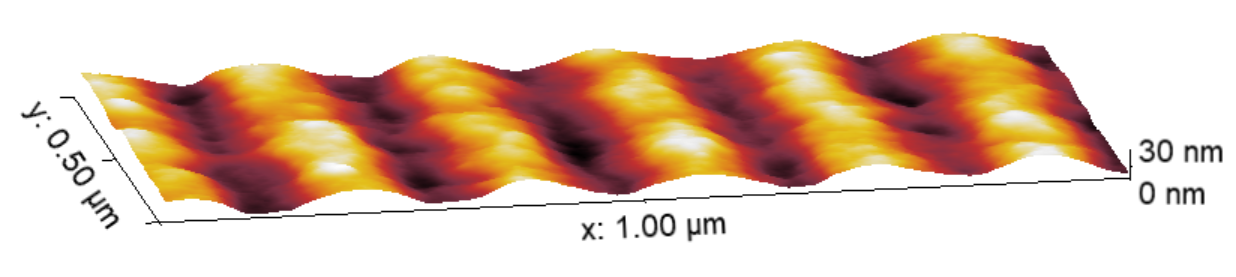
\includegraphics[scale=0.7]{Chapter-1/Figures/OGRESS_capture.PNG}
 \caption[Atomic force micrograph (AFM) of a sinusoidal grating used for sounding-rocket experiments]{AFM of a sinusoidal grating used for sounding-rocket experiments.}\label{fig:OGRESS_AFM}
 \end{figure}
An \emph{atomic force micrograph (AFM)} of one these gratings, which has a groove density of \num{5670} grooves per \si{\mm} ($d \approx \SI{176.4}{\nm}$) and a nickel coat for soft x-ray reflectivity, is shown in \cref{fig:OGRESS_AFM}.\footnote{This image was taken at the Penn State Materials Characterization Laboratory (MCL) \cite{PSU_MRI_CL} using a \textsc{Bruker Dimension Icon}$^{\text{TM}}$ AFM under \textsc{PeakForce Tapping}$^{\text{TM}}$ mode \cite{Xu18}.} 

Holographic gratings ideally would be blazed to sawtooth profile to maximize diffraction efficiency for a particular diffracted angle [\emph{cf.\@} \cref{eq:blaze_wavelength}]. 
A topography that approximates a blazed profile can often be fabricated through holographic recording by tilting the substrate during exposure \cite{Loewen97}. 
Alternatively, a typical holographic grating can be blazed to a sawtooth-like profile by ablating one side of the sinusoidal grooves through directional ion etching to achieve a quasi-blaze profile in the photoresist or the underlying substrate \cite{Loewen97,Aoyagi76,Palmer95}. 
Although this type of grating has been shown experimentally to exhibit a blaze effect in an extreme off-plane mount, they have also been found to perform with lower overall diffraction efficiency in the soft x-ray spectrum than their parent sinusoidal gratings \cite{McEntaffer04,Miles15,Tutt16}. 
This is likely a result of there being extra surface roughness induced by the ion milling process that causes absorption and non-specular scatter [\emph{cf.\@} \cref{sec:rough_surface}]. 

Interference lithography can also be used to define a groove layout in a photoresist for crystallographic etching in silicon [\emph{cf.\@} \cref{sec:crystal_etching}] produces smooth, triangular groove facets \cite{Franke97,Chang03}. 
There are, however, fundamental aspects of this lithographic process that prevent an idealized x-ray reflection grating from being obtained. 
While gratings with $d \lessapprox \SI{100}{\nm}$ can be fabricated using interference lithography in some cases \cite[\emph{cf.\@} \cref{sec:summary_ch5}]{Chang08}, the wavelength of the recording laser, $\lambda_0$, often practically limits $d$ to a few hundred \si{\nm} [\emph{cf.\@} \cref{holographic_groove_spacing}]. 
More importantly, however, a true radial profile for off-plane gratings cannot be produced using this technique because curved grooves are produced when the recording lasers are offset rather than the targeted design, where grooves are straight and continuous but fan outward like spokes on a bicycle wheel \cite{Cash83}. 
With all of this considered, it is worthwhile to explore the capabilities of other techniques in the realm of nanofabrication to find methodology better suited for the task. 

\subsubsection{Electron-Beam Lithography}\label{sec:binary_ebeam}
%%%%%%%%%%%%%%%%%%%%%%%%%%%%%%%%%%%%%%%%%--------------------------------------------------
Direct-write patterning utilizing finely-focused beams of energetic electrons, ions or photons is commonly used in a variety of applications for fabricating photomasks or defining custom layouts in resist that serve as a template for subsequent etching processes. 
Among these techniques, \emph{electron-beam lithography (EBL)} \cite{Chen15,Mohammad2012,Wu10} has been pursued the most for x-ray reflection grating technology due to its ability to pattern custom groove layouts in a resist film with sub-\si{nm} precision combined with its widespread use in nanofabrication facilities and mature stages of technological development. 
Much of the recent work in this area \cite{McCoy18,Miles18,McCoy20,McCurdy20,DeRoo20a,DeRoo20b} has taken place at the Nanofabrication Laboratory of the Penn State Materials Research Institute using an \textsc{EBPG5200} tool for EBL built by \textsc{Raith Nanofabrication} \cite[\emph{cf.\@} \cref{fig:ebeam_tool_pic}]{raith_ebpg,PSU_MRI_nanofab,PSU_MRI_EBL}. 
\begin{figure}
 \centering
 \includegraphics[scale=0.057]{Chapter-1/Figures/ebeam_tool_edit.jpg}
 \caption[The \textsc{EBPG5200} electron-beam lithography (EBL) system installed at the Penn State Nanofabrication Laboratory]{The \textsc{EBPG5200} electron-beam lithography system installed at the Penn State Nanofabrication Laboratory \cite{PSU_MRI_EBL}.}\label{fig:ebeam_tool_pic}
 \end{figure}
Similar to other common EBL tools, the \textsc{EBPG5200} integrates a thermally-assisted, field-emission electron source with a system of electromagnetic lenses to focus a high-quality beam of electrons to a very small spot size \cite{Nakazawa88,Wu10}.  
This occurs under high vacuum to reduce the blurring effect of electrons scattering from gas molecules and moreover, small electric currents and large accelerating voltages generally are required to overcome the mutual electrostatic repulsion of the electrons to achieve a small spot size. 

The \textsc{EBPG5200} in particular uses a \SI{100}{\kilo\volt} accelerating voltage to enable an electron-beam with current measured in nanoamps (\si{\nano\ampere}) to be focused with a diameter less than \SI{10}{\nm} under optimized conditions \cite{PSU_MRI_EBL}. 
Meanwhile, computer-controlled electrostatic deflectors and beam-blanking electrodes in the tool serve to provide lithographic control of the beam so that a groove layout can be patterned serially in a somewhat similar manner to the process of mechanical ruling, but without the physical burnishing process \cite{Chen15,Mohammad2012,Wu10}. 
Direct-write patterning by beam deflection, however, is accessible only up to areas of \SI{1}{\mm} by \SI{1}{\mm} or less in most EBL tools, including the \textsc{EBPG5200}. 
A consequence of this is that for x-ray reflection gratings, which generally have patterned areas greatly exceeding \SI{1}{\mm\squared}, stage motion is required for a large number of these \emph{write fields} to be stitched together. 
This must be carried accurately because misalignments between these patterned areas lead to groove spacing error, and in principle, this can contribute to a degradation in $\mathscr{R}$ \cite{Dougherty01,DeRoo20b}. 
While this process enables the creation of custom, high-precision layouts for x-ray reflection gratings, it also leads to long manufacturing times and hence high laboratory costs for gratings of substantial size. 
It is for this primary reason that EBL is practically only used for the fabrication of a master grating while nanoimprint lithography [\emph{cf.\@} \cref{sec:nanoimprint}] is used to produce replicas for a spectrometer. 
%It is for this primary reason that EBL is practically only used for the fabrication of a master grating while techniques in nanoimprint lithography are used to produce replicas for a grating spectrometer [\emph{cf.\@} \cref{sec:nanoimprint}]. 

As alluded to in \cref{sec:holographic}, pattern resolution in holographic recording is limited fundamentally by the wavelength of the radiation used for lithographic exposure, $\lambda_0$. 
In contrast, pattern feature sizes in EBL are limited not by diffraction but rather by other factors such as the accuracy of the tool, the stability and size of the focused beam and additionally, the nature of the resist material \cite{Vieu00,Broers96,Manfrinato14}. 
This can be understood by considering the effective wavelength of a hypothetical mono-energetic beam of electrons, which is calculated by equating the relativistic kinetic energy of an electron to the change in electrostatic energy provided by a potential difference, $V_0$, that represents the accelerating voltage in an EBL tool \cite{Landau75}: 
\begin{subequations}
\begin{equation}\label{eq:rel_KE_voltage_balance}
 m_e c_0^2 \left( \frac{1}{\sqrt{1-\frac{v^2}{c_0^2}}} - 1 \right) = q_e V_0 ,
 \end{equation}
where $m_e$ is the electron rest mass, $c_0$ is the speed of light, and $q_e$ is the elementary charge, while $v$ is the speed of the electron. 
Solving \cref{eq:rel_KE_voltage_balance} for $v$ shows that an electron accelerated by a voltage of $\SI{100}{\kilo\volt}$ in the \textsc{EBPG5200} is relativistic: 
\begin{equation}
 v = c_0 \sqrt{1 - \left( \frac{1}{1 + \frac{q_e V_0}{m_e c_0^2}} \right)^2} \approx \num{0.548} c_0 \quad \text{for } V_0 = \SI{100}{\kilo\volt} .
 \end{equation}
Moreover, its relativistic momentum is given by 
\begin{equation}
 p = \frac{m_e v}{\sqrt{1 - \frac{v^2}{c_0^2}}} = m_e c_0 \sqrt{\left( 1 + \frac{q_e V_0}{m_e c_0^2} \right)^2 - 1} 
 \end{equation}
and then the \emph{de Broglie wavelength} for an electron, determined from 
\begin{equation}\label{eq:electron_wavelength}
 \lambda_e = \frac{h}{p} = \frac{\lambda_C}{\sqrt{\left( 1 + \frac{q_e V_0}{m_e c_0^2} \right)^2 - 1}} \quad \text{with } \lambda_C \equiv h / m_e c_0 \approx \SI{2.43}{\pm} ,
 \end{equation}
shows that an electron accelerated to \SI{100}{\kilo\electronvolt} has an effective wavelength of about \SI{3.7}{\pm}, indicating that from the standpoint of scalar diffraction, a mono-energetic beam of electrons can be thought of as being analogous to a mono-chromatic beam of electromagnetic radiation but with a much smaller wavelength. 
\end{subequations}
In practice, field-emission electron sources in modern EBL tools are characteristic of energy dispersion on a sub-\si{\electronvolt} level; this low-energy dispersion enables an electron-beam with electric current measured in \si{\nano\ampere} to be very finely focused by electromagnetic lenses \cite{Pala16}.

In a common EBL process for grating manufacture, a silicon wafer or a specialized optical flat is coated with a film of resist that acts as the recording medium for the electron beam \cite{Chen15,Mohammad2012,Wu10}. 
This film is typically a layer of polymers or copolymers that constitute a solid, predominantly amorphous, material network with a thickness of a few hundred \si{\nm} or more. 
A commonly used material is \emph{poly(methyl methacrylate)} (PMMA), which is a thermoplastic polymer composed of many repeating units of the monomer \emph{methyl methacrylate} (MMA; \ce{C5H8O2}) \cite{Hatzakis69,Greeneich75,Broers78,Ali15}. 
\begin{figure}
 \centering
 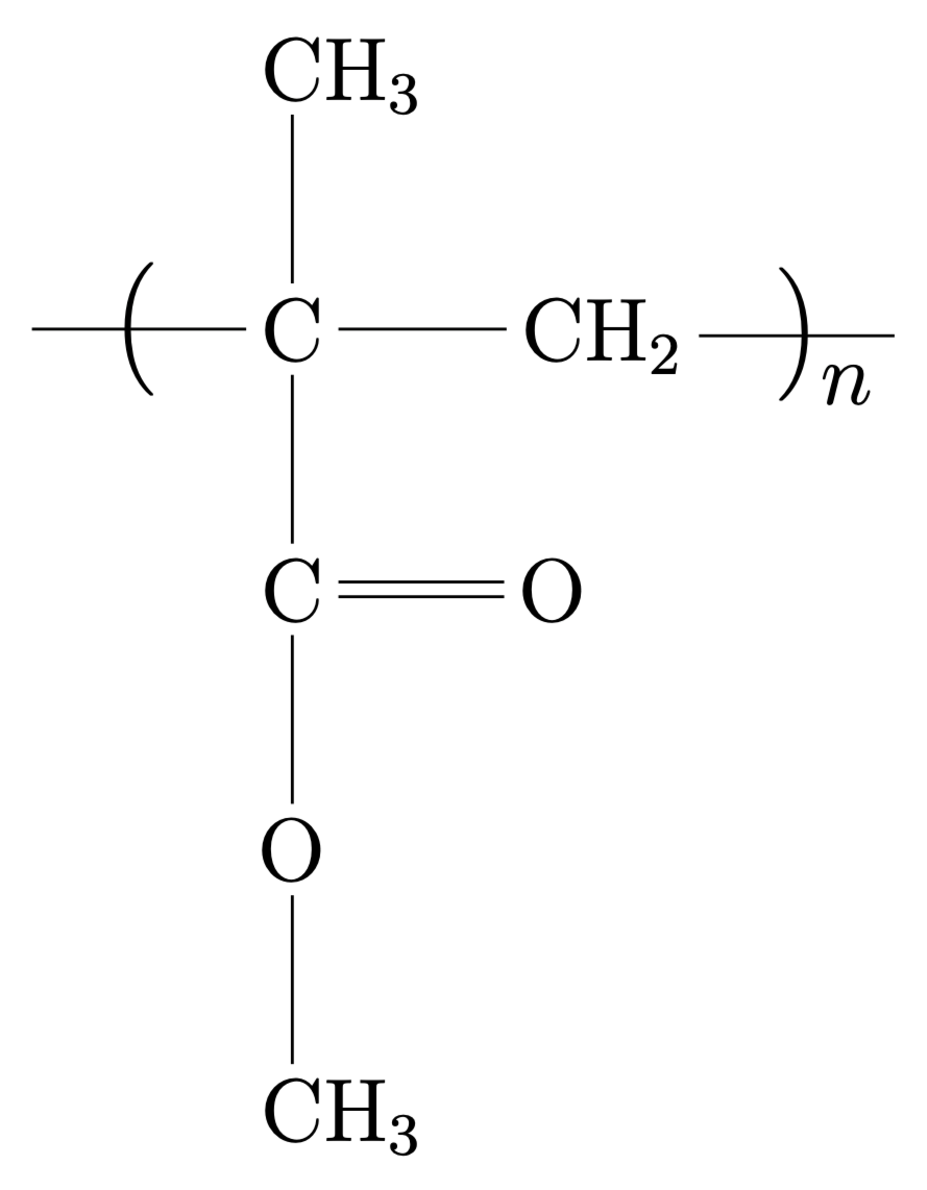
\includegraphics[scale=0.4]{Chapter-1/Figures/PMMA.pdf}
 \caption[Structural formula of poly(methyl methacrylate) (PMMA).]{Structural formula of poly(methyl methacrylate) (PMMA). The average molecular weight, $M_w$, of PMMA resist depends directly on the length of these polymer chains, which is indicated by the degree of polymerization, $n$, that represents the number of monomers bonded together.}\label{fig:PMMA}
 \end{figure}
The structural formula for this macromolecule is drawn in \cref{fig:PMMA}, where MMA monomers with molar mass $M_0 \approx \SI{100}{\gram\per\mole}$ are covalently bonded together at the sites marked by brackets to form a linear polymer chain. 
In practice, synthesized PMMA contains a spread of polymer chain lengths; the number-averaged molecular mass is defined as 
\begin{subequations}
\begin{equation}
 M_n \equiv \frac{\sum_j N_j M_j}{\sum_j N_j} ,
 \end{equation}
where $N_j$ is the number of PMMA molecules of mass $M_j$ so that the average number of monomers bonded together in polymer chains is $M_n / M_0$, which is known as the \emph{degree of polymerization}. 
However, resist molecular weight provided by chemical manufacturers is usually a mass-averaged molar mass: 
\begin{equation}\label{eq:weight_avg_molecular_weight}
 M_w \equiv \frac{\sum_j N_j M_j^2}{\sum_j N_j M_j} ,
 \end{equation}
\end{subequations}
and this quantity is related to $M_n$ through the \emph{dispersity} of the material defined as $\DJ \equiv M_w / M_n \geq 1$, which is a measure of the polymer chain length distribution in the resist with $\DJ = 1$ corresponding to a uniform distribution \cite{Stepto09,Kirchner19}. %change $\text{PDI} = 1$ to $\DJ = 1$
A thin film of glass-state PMMA with a known value of $M_w$ is typically achieved by spin-coating a substrate with a solution of the polymer cast in a solvent that is removed with a hotplate bake [\emph{cf.\@} \cref{sec:TASTE}]. 

The electron-beam recording mechanism in PMMA and other positive-tone resists such as ZEP520A\footnote{This material is a copolymer of \emph{$\alpha$-chloromethacrylate} and \emph{$\alpha$-methylstyrene} with the chemical formula \ce{C13H6O2Cl} \cite{Czaplewski11}. Available from \textsc{Zeon Chemicals L.P.}, it is a thermoplastic resist similar to PMMA, but with improved dry etch selectivity and other differing parameters.} starts with polymer chain scission by high-energy electrons, which serves to lower $M_w$ in the resist locally \cite{Dobisz00,Greeneich75}. 
Lithographic electrons, such as those accelerated to \SI{100}{\kilo\electronvolt} in the \textsc{EBPG5200}, are energetic enough to forward-scatter through relatively thin resist layers with negligible intensity loss so that $M_w$ can be considered uniform throughout the depth of the exposed film \cite{Schleunitz10,Kirchner19}. 
The degree to which $M_w$ is reduced essentially depends on the number of electrons available for polymer chain scission in an exposed area, which is quantified by an electron dose, $D$ (usually given in units of \si{\micro\coulomb\per\cm\squared}). 
However, in addition to breaking polymer chains into fragments as they forward-scatter through a layer of resist, lithographic electrons back-scatter through the substrate, causing the resist to be inadvertently dosed over distances on the order of \SI{10}{\um} through the phenomenon known as the \emph{proximity effect} in EBL \cite{Pavkovich86,Wu10}. 
Algorithms for proximity effect correction, such as those provided by the \textsc{Layout BEAMER} software package (\textsc{GenISys GmbH}) \cite{beamer}, can be used to determine how $D$ should be adjusted across a layout to achieve a desired pattern in the resist. 
In any case, exposed PMMA that is fragmented to a sufficiently low $M_w$ is soluble in a suitable wet developer, such as a mixture of \emph{methyl isobutyl ketone} (MIBK; \ce{C6H12O}) and \emph{isopropyl alcohol} (IPA; \ce{C3H8O}), while unexposed resist with relatively large $M_w$ is virtually unaffected \cite{miller-chou03,Pratt75}. 
This enables PMMA with $M_w$ on the order of hundreds of \si{\kilogram\per\mole} to be used as a positive-tone resist in EBL, where, with a appropriate choice for $D$ and wet development parameters, exposed resist can be etched down to the substrate during wet development while the unexposed resist remains intact \cite{Greeneich75,Vutova01,Schift10,Kirchner19}. 

The end result of a standard EBL process for grating manufacture is a bi-level topography featuring lines and spaces of remaining resist and cleared substrate that define a groove spacing, $d$. 
For such a pattern to function as reflection grating, however, the layout is usually transferred into a more robust material such as an underlying substrate, which is illustrated schematically for a simplified fabrication process in \cref{fig:laminar_fab} \cite{Zeitner12}. 
\begin{figure} 
\centering
\includegraphics[scale=1.08]{Chapter-1/Figures/laminar_fab1.mps}
\includegraphics[scale=1.08]{Chapter-1/Figures/laminar_fab2.mps}
\includegraphics[scale=1.08]{Chapter-1/Figures/laminar_fab3.mps}
\includegraphics[scale=1.08]{Chapter-1/Figures/laminar_fab4.mps}
\caption[Outline of a simplified laminar grating fabrication recipe that uses EBL]{Outline of a simplified laminar grating fabrication recipe that uses EBL to define a groove layout.}\label{fig:laminar_fab}
\end{figure}
An AFM\footnote{As in \cref{fig:OGRESS_AFM}, this image was taken at the Penn State MCL \cite{PSU_MRI_CL} using a \textsc{Bruker Dimension Icon}$^{\text{TM}}$ AFM under \textsc{PeakForce Tapping}$^{\text{TM}}$ mode \cite{Xu18}.} of such a grating pattern is shown in \cref{fig:laminar_AFM}. 
\begin{figure} 
 \centering
 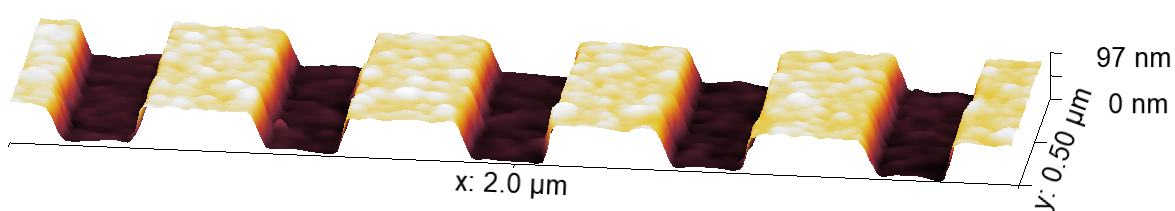
\includegraphics[scale=0.5]{Chapter-1/Figures/laminar_amorphous_AFM.PNG}
 \caption[AFM of a laminar grating dry etched in amorphous silicon]{AFM of a laminar grating dry etched in amorphous silicon.}\label{fig:laminar_AFM}
 \end{figure}
This grating with $d = \SI{400}{\nm}$ was fabricated by staff at the Penn State Nanofabrication Laboratory \cite{PSU_MRI_nanofab} by using a dry-etch process (\emph{i.e.}, reactive ion etching)\footnote{Briefly, a \emph{dry etch} process uses a plasma driven by a radio-frequency electromagnetic field to etch a surface through the bombardment of ions. Due to the directional nature of the ions, such a process is anisotropic in the sense material is etched downward. However, \emph{reactive ion etching (RIE)} has the added component that ions react chemically to some degree with the surface and this introduces an isotropic component to the etch \cite{Franssila10}.\label{footnote:dry_etch_RIE}} to transfer the resist into a layer of amorphous silicon (not shown in \cref{fig:laminar_fab}) coated on a silicon wafer in a manner similar to the grating tested for soft x-ray spectral resolving power by DeRoo, et~al.~\cite{DeRoo20a}. 

The diffraction-efficiency behavior of a laminar grating depends on the angles of incidence, but in any case, the result is that certain propagating orders in principle are suppressed and hence a true blaze response is not achieved. %\footnote{Depending on the dry-etch selectivity of the resist used for EBL, an underlying layer of a more robust material (\emph{e.g.}, a silicon nitride footnote~\ref{footnote:nitride_mask}]) may be required to serve as a mask for the silicon etch.}
For angles of incidence close to $\alpha = 0$ in \cref{fig:conical_reflection_edit}, the scenario can be described approximately as a binary phase grating [\emph{cf.\@} \cref{eq:square_principle}], where radiation picks up a phase shift as it traverses the depth of the grating grooves; the result, according to this scalar treatment of diffraction, is a \emph{sinc-squared} modulation of the far-field intensity that depends on both the groove depth and the grating duty cycle. 
On the other hand, a large $\alpha$ in an extreme off-plane mount preferentially illuminates the sidewall of the laminar groove facets, which can lead to high efficiency in high order similar to a blazed grating, but still not without the suppression of other propagating orders. 
A sawtooth topography with a sharp apex and a well-defined blaze angle, $\delta$, is instead required to achieve high efficiency over a range of orders and to better customize the grating for a bandpass of interest. 
However, a laminar grating etched in silicon can be used as a template for ion milling, which ablates these facets at an angle to create a sawtooth-like topography \cite{Johnson79,Liu13}. 
While this is the subject of ongoing research at Penn State \cite{Miles2019_ion_mill}, an alternative, well-established strategy to achieving a grating blaze for a groove layout defined by EBL is crystallographic etching, which is described next. 

\subsubsection{Crystallographic Etching in Silicon}\label{sec:crystal_etching}
%%%%%%%%%%%%%%%%%%%%%%%%%%%%%%%%%%%%%%%%%--------------------------------------------------
A groove layout in a resist film patterned by virtually any lithography can be used to define a mask for anisotropic wet etching in mono-crystalline silicon, typically with a solution of \emph{potassium hydroxide} (\ce{KOH}), to achieve high-fidelity, sawtooth-shaped groove facets. 
This technique has been pursued previously to fabricate blazed reflection gratings for x-ray telescope applications \cite{Franke97,Chang03,Chang04,McEntaffer13,Peterson15,DeRoo16thesis,DeRoo16,Miles18} and multilayer-coated blazed gratings for extreme UV and x-ray monochromator applications \cite{Voronov10,Voronov11,Voronov16}, where in each case, either interference lithography, EBL or nanoimprint lithography [\emph{cf.\@} \cref{sec:holographic,sec:binary_ebeam,sec:nanoimprint}] was used to pattern a groove layout that was transferred by dry etch into an underlying hardmask layer\footnote{In many cases this etch mask is composed of stoichiometric silicon nitride (\ce{Si3N4}) or some other composition of the material (\ce{Si_{x}N_{y}}). A silicon-nitride film can be coated on a silicon wafer using an optimized, \emph{low-pressure chemical vapor deposition (LPCVD)} process, where gaseous chemical precursors are injected into a vacuum chamber while the wafer is heated to promote chemical reactions to occur at its surface to grow a film of a specified thickness on the wafer (typically a few tens of \si{\nm}) \cite{Franssila10}.\label{footnote:nitride_mask}} and then, following the removal of native oxide on the silicon surface (\ce{SiO2}), the crystal structure of a silicon substrate through a wet \ce{KOH} etch.\footnote{This can be carried out through a wet \emph{buffered oxide etch (BOE)} that consists of \emph{hydrofluoric acid} (\ce{HF}) diluted in \emph{ammonium fluoride} (\ce{NH4F}) \cite{Franssila10}.\label{footnote:buffered_oxide_etch}}
Such a process is described as anisotropic in the sense that \ce{KOH} etch rates in crystalline silicon depend strongly on crystallographic direction. 
If the groove layout is aligned with the crystal structure of the substrate appropriately, this manifests as a collection of atomically-smooth troughs that appear similar to a triangular sawtooth when viewed edge-on \cite{Tsang75,Sato99,Franssila10,Gosalvez15}.
The effective blaze angle for a reflection grating then depends on the surface-normal orientation of the wafer used for etching as well as the groove direction relative to crystallographic directions on the surface of the wafer \cite{McEntaffer13,DeRoo16,Miles18}. 

The ideal result of a \ce{KOH}-etching process can be envisioned by considering the \emph{face-centered cubic} crystal structure of silicon, which is illustrated\footnote{These diagrams were generated by T.\ Wood using \textsc{CrystalMaker X} \cite{crystal_maker,Palmer_CM}.} in \cref{fig:crystal_structure}. 
To start, the unit cell of this cubic crystal structure can be defined using an orthogonal set of principal-axis vectors, $\mathbold{a}$, $\mathbold{b}$ and $\mathbold{c}$, that each have identical magnitudes given by the lattice constant of silicon (\emph{i.e.}, $\abs{\mathbold{a}} = \abs{\mathbold{b}} = \abs{\mathbold{c}} = a_{\text{Si}} \approx \SI{0.54}{\nm}$) and directions given by $[ 1 0 0 ]$, $[ 0 1 0 ]$ and $[ 0 0 1 ]$, respectively [\emph{cf.\@} \cref{fig:crystal_structure}]. %\footnote{More generally, the directional distance between any two points on the crystal lattice can be written in this basis as $\mathbold{R} = u \mathbold{a} + v \mathbold{b} + w \mathbold{c}$, where $u$, $v$ and $w$ are integers \cite{Trolier-McKinstry17}.}
\begin{figure}
 \centering
 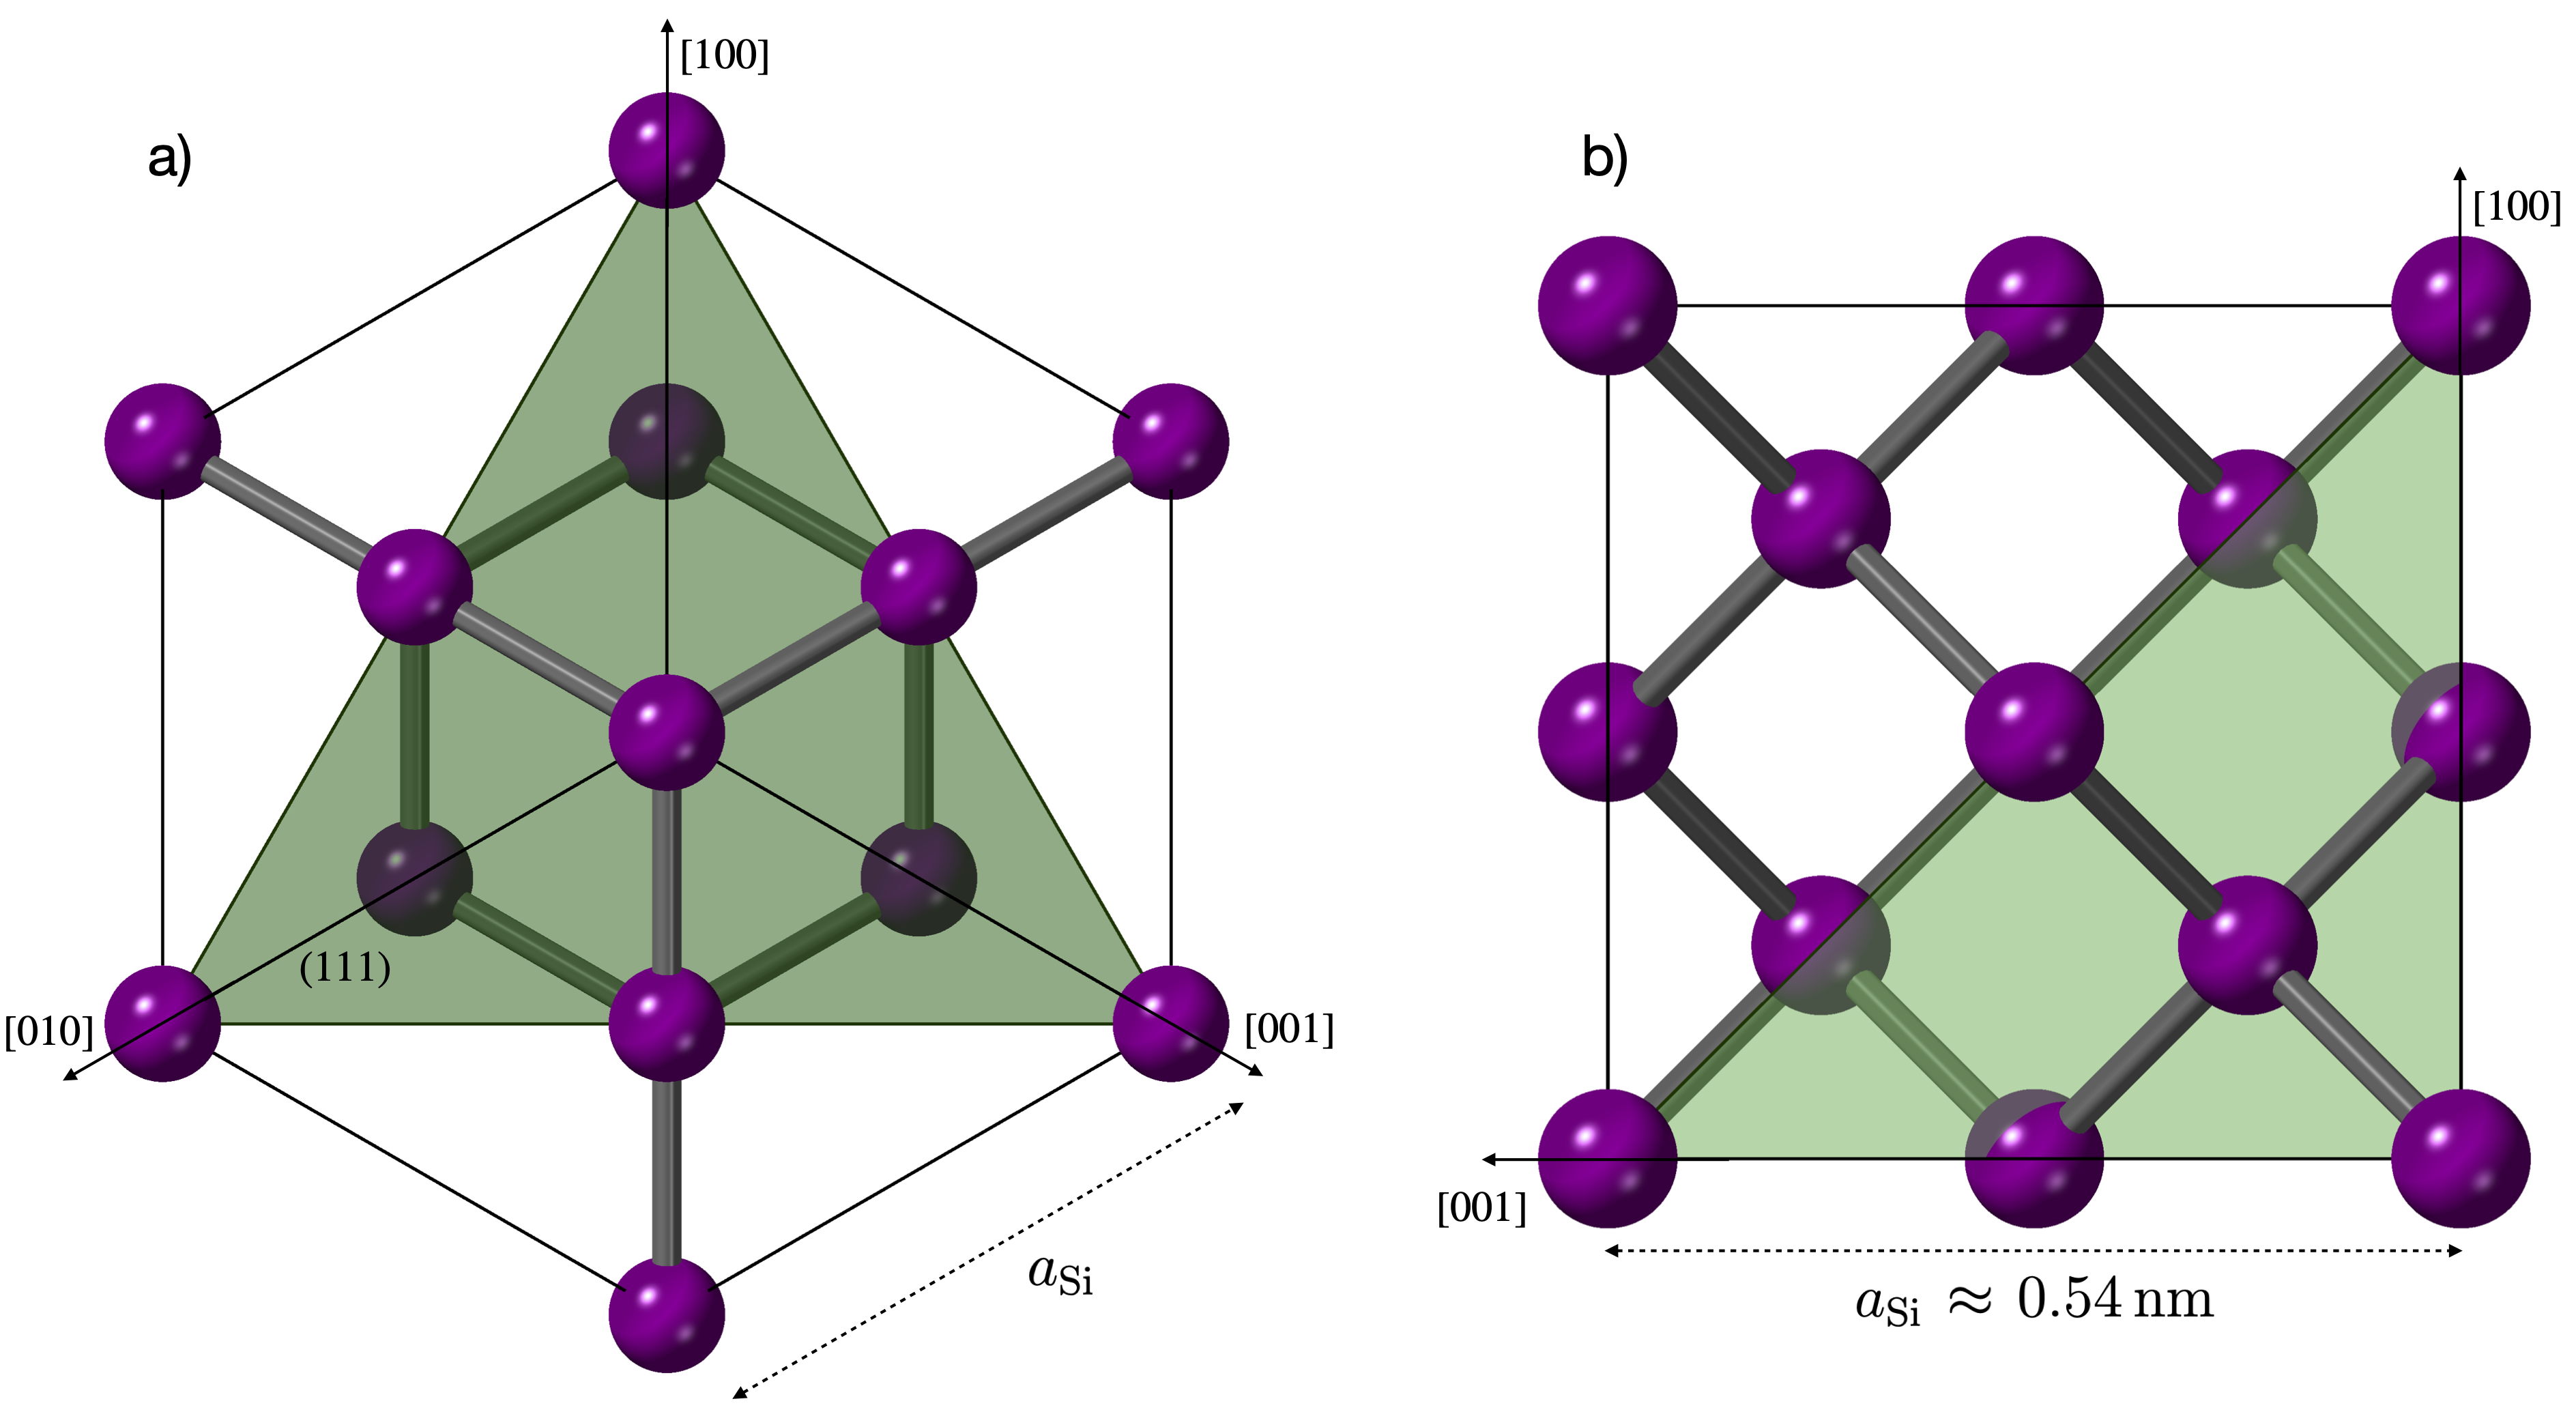
\includegraphics[scale=0.235]{Chapter-1/Figures/crystal_fig1.png}
 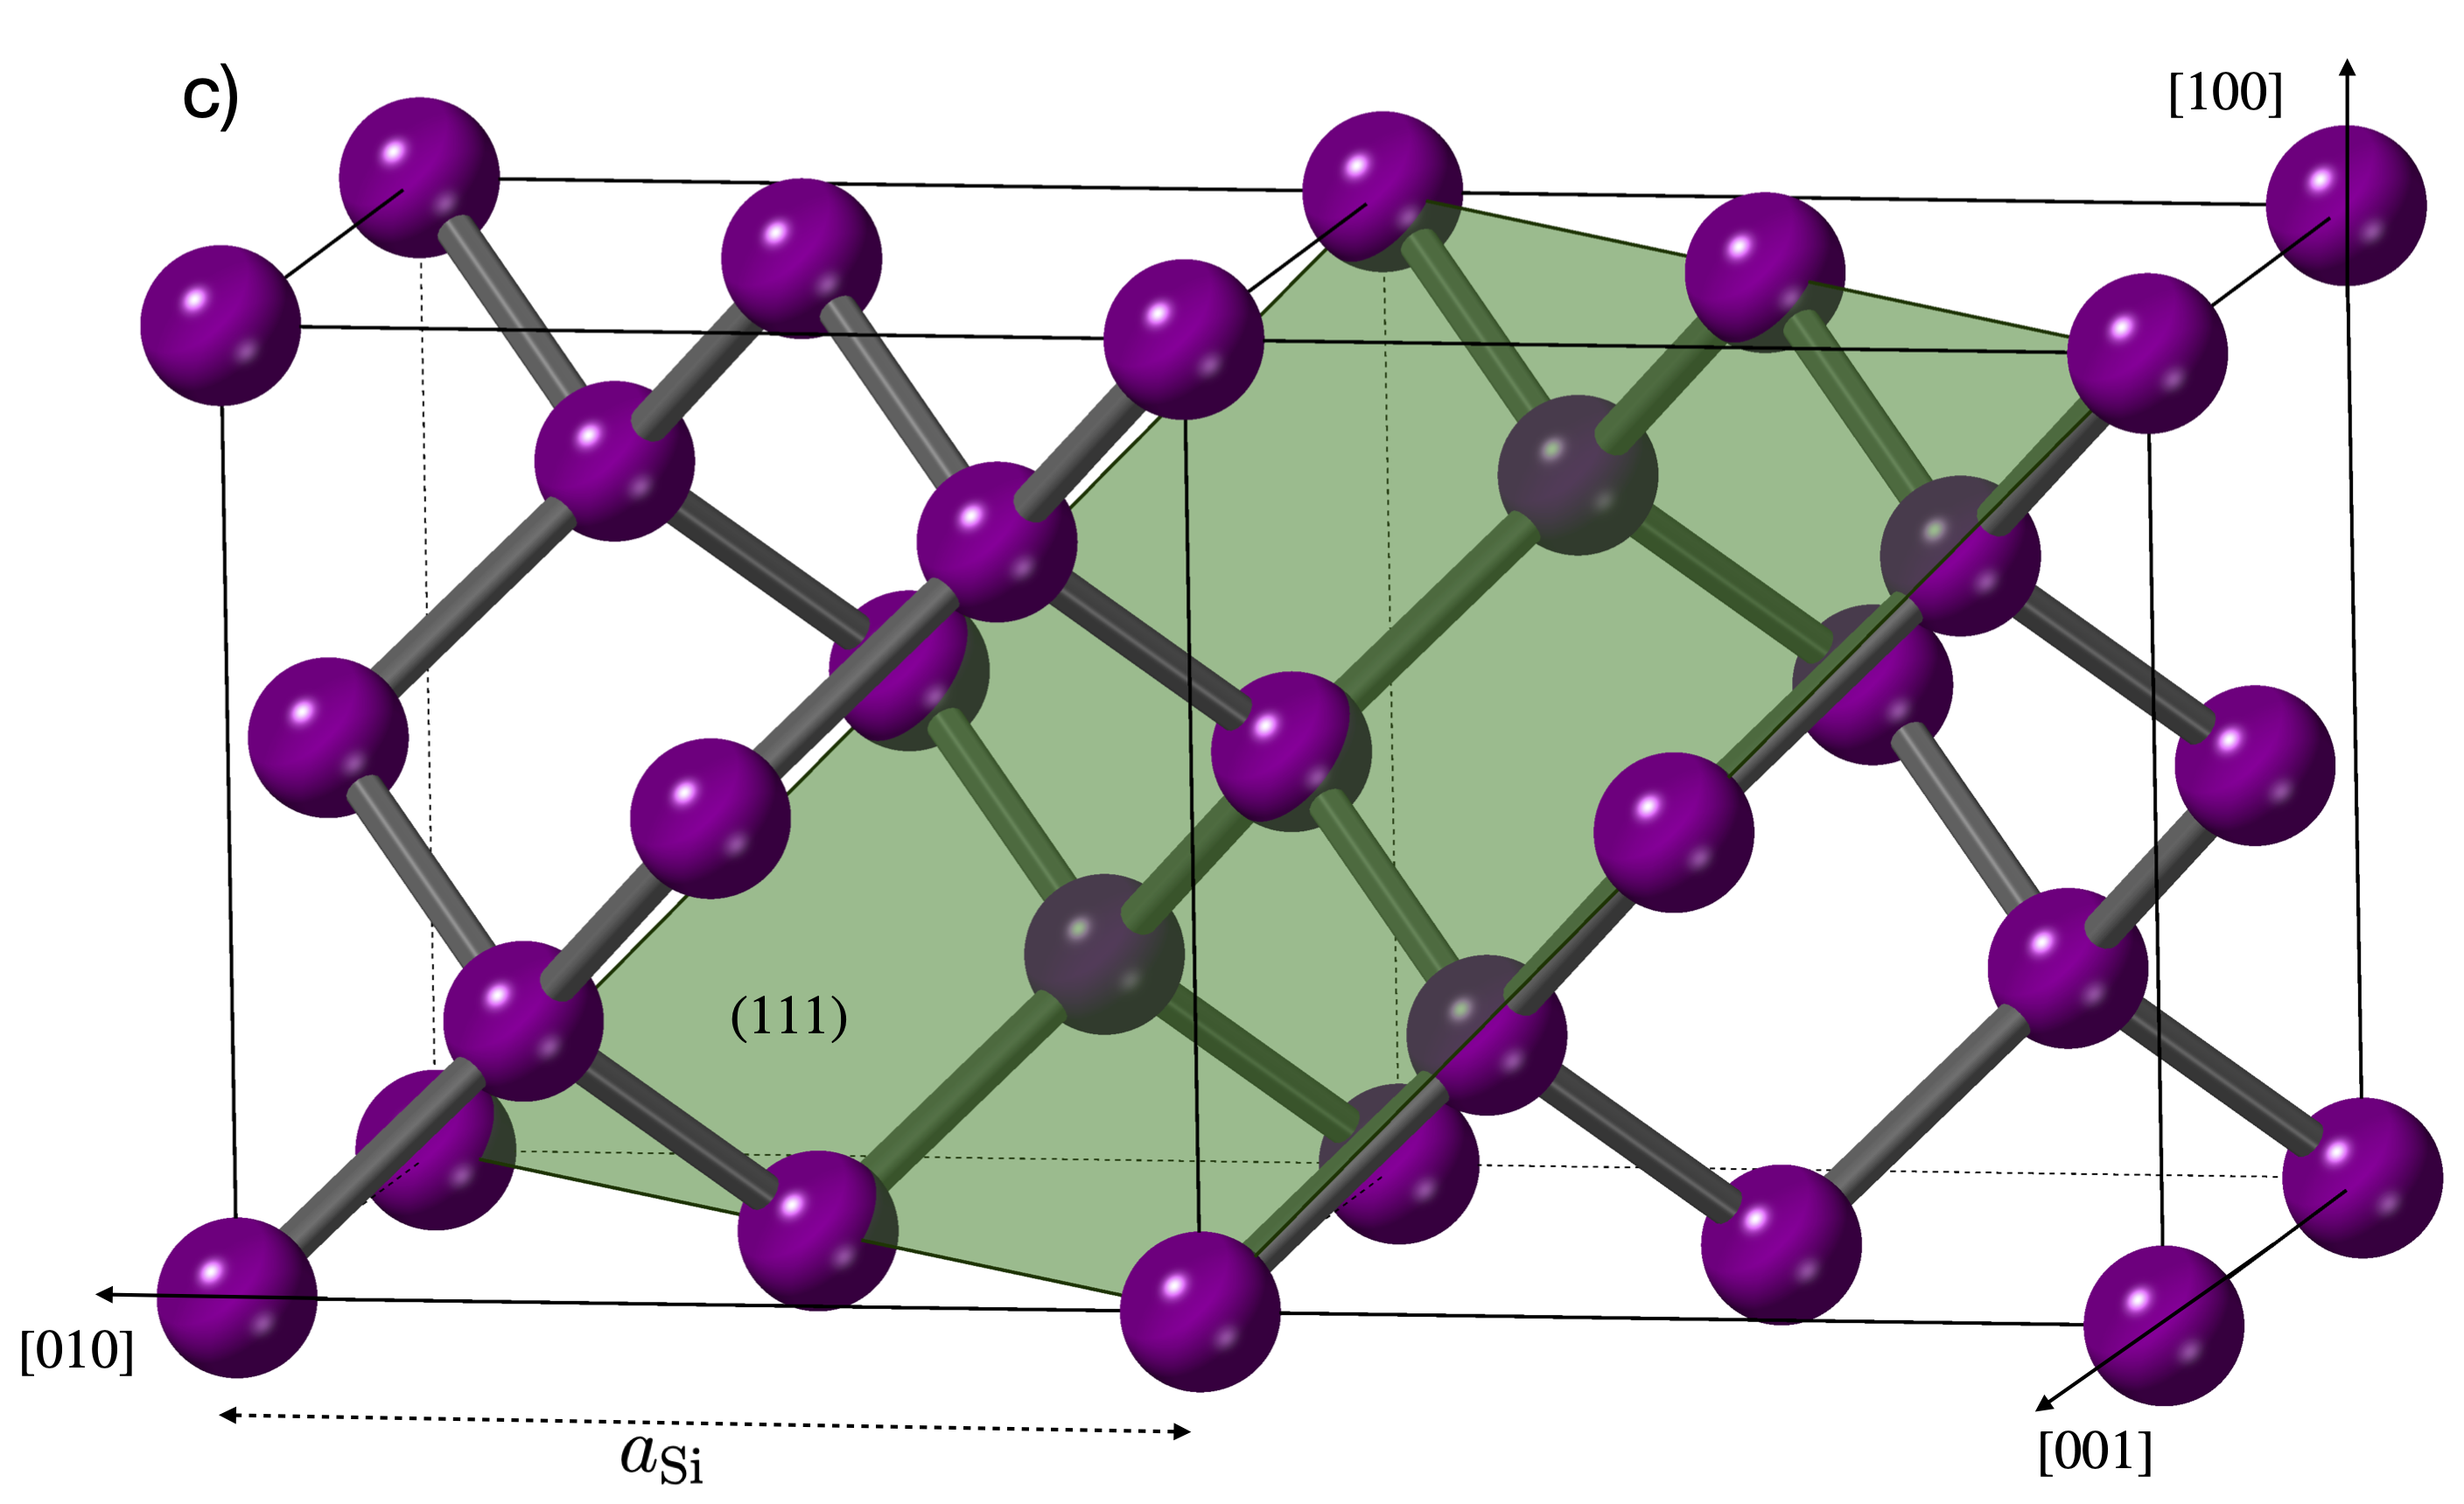
\includegraphics[scale=0.235]{Chapter-1/Figures/crystal_fig2.png}
 \caption[Face-centered cubic structure of silicon (credit: T.\ Wood using \textsc{CrystalMaker})]{Three views of the face-centered cubic structure of silicon, where $a_{\text{Si}} \approx \SI{0.54}{\nm}$ is the lattice constant, cube faces are $\{ 100 \}$ planes, purple spheres represent silicon atoms and gray bars indicate covalent bonds while a $(111)$ plane is shown in green: a) down the $[ 111 ]$ axis of a single unit cell, b) down the $[ 010 ]$ axis of a single unit cell and c) two adjacent cells. Image credit: T.\ Wood using \textsc{CrystalMaker X} \cite{crystal_maker}.}\label{fig:crystal_structure} 
 \end{figure}
Along with $[ \overline{1} 0 0 ]$, $[ 0 \overline{1} 0 ]$ and $[ 0 0 \overline{1} ]$ (where an overbar indicates a negative integer), $[ 1 0 0 ]$, $[ 0 1 0 ]$ and $[ 0 0 1 ]$ form a family of crystallographic directions that are equivalent by symmetry; this is denoted by $\langle 1 0 0 \rangle$ \cite{Franssila10,Trolier-McKinstry17}. %\footnote{In regard to crystallographic directions and planes, an overbar indicates a negative integer. Moreover, this notation holds for any $\langle u v w \rangle$ but the number of symmetry-related directions may vary.} 
A crystallographic plane that intersects the principal-axis vectors at $\mathbold{a} / h$, $\mathbold{b} / k$ and $\mathbold{c} / \ell$ is represented as $(h k \ell)$, where $h$, $k$ and $\ell$ are integers known as \emph{Miller indices}, and in the special case of a cubic crystal, $[ h k \ell ]$ and $(h k \ell)$ are always orthogonal such that the spacing between successive $(h k \ell)$ planes is given by \cite{Trolier-McKinstry17} 
\begin{equation}\label{eq:d_hkl}
 d_{h k \ell} = \frac{a_{\text{Si}}}{\sqrt{h^2 + k^2 + \ell^2}} . 
 \end{equation} 
Using $\{ h k \ell \}$ to denote a family of crystallographic planes that are equivalent by symmetry, $\{ 1 1 1 \}$ planes include $( 1 1 1 )$, $( \overline{1} 1 1 )$, $( 1 \overline{1} 1 )$, $( 1 1 \overline{1} )$, $( 1 \overline{1} \overline{1} )$, $( \overline{1} 1 \overline{1} )$, $( \overline{1} \overline{1} 1 )$ and $( \overline{1} \overline{1} \overline{1} )$ with a $( 1 1 1 )$ plane shown in \cref{fig:crystal_structure} as an example. 

\ce{KOH} is known to etch crystalline silicon along $\langle 1 1 1 \rangle$ directions at a rate much lower than all other families of crystallographic directions, and as a result, the $\{ 1 1 1 \}$ planes that intersect with the edges of the etch-mask layout are left exposed by the etch \cite{Franssila10,Gosalvez15}. 
To discuss this, the most common wafer geometry used for \ce{KOH} etching is one with a $\langle 100 \rangle$ surface normal and grooves aligned along any $\langle 011 \rangle$ direction, which is illustrated in \cref{fig:KOH_geo}. 
\begin{figure}
 \centering
 \includegraphics[scale=0.9]{Chapter-1/Figures/UV1.mps}
 \caption[Geometry for \ce{KOH} etching in a $\langle 100 \rangle$-oriented silicon wafer]{Geometry for \ce{KOH} etching in a $\langle 100 \rangle$-oriented silicon wafer. The surface of the wafer is a $\{ 100 \}$ equivalent plane with a normal direction taken to be $[100]$. In this projection, the $[01\overline{1}]$ direction points out of the page while $(111)$ and $(1\overline{1} \overline{1})$ are the exposed $\{ 111 \}$ planes, defining an angle $\theta = 70.53^{\circ}$. The result is a symmetric sawtooth with a nominal blaze angle $\delta = 54.74^{\circ}$.}\label{fig:KOH_geo}
 \end{figure}
Taking the wafer surface normal to be $[100]$ with $[01\overline{1}]$ as the groove direction, the $\{ 111 \}$ planes exposed by a \ce{KOH} etch in this case are $(111)$ and $(1\overline{1} \overline{1})$, which intersect at an angle of $\theta = 70.53^{\circ}$. 
This can be seen by carrying out the dot product between two normalized vectors representing the $[111]$ and $[1 \overline{1} \overline{1}]$ directions, which are normal to the $(111)$ and $(1\overline{1} \overline{1})$ planes, and then taking the supplementary angle: 
\begin{equation}\label{eq:Si_angle}
 \frac{1}{\sqrt{3}} \begin{pmatrix} 1 & -1 & -1 \end{pmatrix}
 \frac{1}{\sqrt{3}} \begin{pmatrix} 1 \\ 1 \\ 1 \end{pmatrix} = -\frac{1}{3} = \cos \left( \pi - \theta \right) \implies \theta = 70.53^{\circ} . 
\end{equation}
Meanwhile, the angle between the wafer surface and both exposed $\{ 111 \}$ planes in the crystal is $\left( 180^{\circ} - \theta \right) / 2$ [\emph{cf.\@} \cref{fig:KOH_geo}]:
\begin{equation}\label{eq:100_angle}
 \frac{1}{\sqrt{3}} \begin{pmatrix} 1 & 1 & 1 \end{pmatrix}
 \begin{pmatrix} 1 \\ 0 \\ 0 \end{pmatrix} = \frac{1}{\sqrt{3}} = \cos \left( \delta \right) \implies \delta = 54.74^{\circ} ,
 \end{equation}
which defines $\delta$ of the symmetric sawtooth produced by such an etch and indicates that the distance between $\{ 111 \}$ planes is $d_{111} \equiv a_{\text{Si}}/\sqrt{3} \approx \SI{0.31}{\nm}$ [\emph{cf.\@} \cref{eq:d_hkl}]. 

Asymmetric sawtooth profiles with blaze angles other than $\delta = 54.74^{\circ}$ can be obtained by choosing an appropriate off-axis-cut silicon wafer with a surface-normal orientation rotated from $[100]$ about the axis coincident with the groove direction, $[01\overline{1}]$, so that $(111)$ and $(1\overline{1} \overline{1})$ are still the exposed $\{ 111 \}$ planes that define the angle $\theta$. 
\begin{figure}
 \centering
 \includegraphics[scale=1.4]{Chapter-1/Figures/UV3.mps}
 \caption[Various wafer orientations that are confined to a plane orthogonal to $\langle 011 \rangle$.]{Various wafer orientations that are confined to a plane orthogonal to $\langle 011 \rangle$. Each of these can be used to etch asymmetric sawtooth topographies into crystalline silicon using \ce{KOH} provided that the grating grooves are aligned with a $\langle 011 \rangle$ direction on the surface of the wafer.}\label{fig:KOH_angles}
 \end{figure}
This is demonstrated in \cref{fig:KOH_angles}, where as in the $\langle 100 \rangle$ case shown in \cref{fig:KOH_geo}, the $\langle 011 \rangle$ direction pointing out of the page is taken to be $[01 \overline{1}]$ while the relevant $\langle 111 \rangle$ directions are still $[111]$ and $[1 \overline{1} \overline{1}]$, which intersect at an angle $180^{\circ} - \theta = 109.47^{\circ}$ [\emph{cf.\@} \cref{eq:Si_angle}]. 
As indicated by \cref{fig:KOH_angles}, a series of vectors representing other wafer orientations also lay in this plane defined by $[111]$ and $[1\overline{1} \overline{1}]$. %, along with $[100]$.  
While a $[100]$ surface normal bisects these two $\langle 111 \rangle$ directions at an angle $\delta = 54.74^{\circ}$ [\emph{cf.\@} \cref{eq:100_angle}], those with crystallographic directions such as $[211]$ and $[311]$ intersect with $[111]$ at a smaller blaze angle, $\delta$, and $[1\overline{1} \overline{1}]$ at a different, steeper angle, $\bar{\delta} = 180^{\circ} - \theta - \delta$, to yield asymmetric sawtooth profiles that are rotated versions of the $\langle 100 \rangle$ case. 

With the angle $\theta$ defined by $\{ 111 \}$ plane intersections as in \cref{fig:KOH_geo}, the blaze angles produced by some of these off-axis wafer orientations are listed in \cref{tab:off_axis_si}. 
\begin{table}[]
 \centering
 \caption{Blaze angles ($\delta$) and corresponding opposite angles ($\bar{\delta} = 180^{\circ} - \theta - \delta$) on asymmetric sawtooth patterns generated by various wafer orientations with grooves aligned along $\langle 011 \rangle$ on the wafer surface.}\label{tab:off_axis_si}
 \begin{tabular}{ccc}
 \toprule
 wafer orientation & blaze angle ($\delta$) & opposite angle ($\bar{\delta}$)  \\ \midrule
 $\langle 211 \rangle$      & $19.47^{\circ}$        & $90^{\circ}$    \\
 $\langle 311 \rangle$      & $29.5^{\circ}$         & $79.97^{\circ}$ \\
 $\langle 411 \rangle$      & $35.26^{\circ}$        & $74.21^{\circ}$ \\
 $\langle 511 \rangle$      & $38.94^{\circ}$        & $70.53^{\circ}$ \\
 $\langle 100 \rangle$      & $54.74^{\circ}$        & $54.74^{\circ}$ \\ \bottomrule
\end{tabular}
\end{table}
A blaze angle of $\delta \approx 30^{\circ}$, for example, can be obtained using a $\langle 311 \rangle$-oriented wafer, which by definition, can be described using a vector that is rotated $25.24^{\circ}$ from $\langle 100 \rangle$, toward $\langle 111 \rangle$ in the plane orthogonal to $\langle 011 \rangle$ (\emph{i.e.}, the groove direction). 
\begin{figure}
 \centering
 \includegraphics[scale=0.9]{Chapter-1/Figures/UV_rev1.mps}
 \caption[Geometry for \ce{KOH} etching in a $\langle 311 \rangle$-oriented silicon wafer]{Geometry for \ce{KOH} etching in a $\langle 311 \rangle$-oriented silicon wafer. The surface of the wafer is a $\{ 311 \}$ equivalent plane with a normal direction taken to be $[311]$. In this projection, the $[01\overline{1}]$ direction points out of the page while $(1\overline{1} \overline{1})$ and $(111)$ are the exposed $\{ 111 \}$ planes. Here, the $(111)$ surface acts as the blazed groove facet with a nominal blaze angle of $\delta = 29.5^{\circ}$ while the $(1\overline{1} \overline{1})$ plane defines a $\bar{\delta} = 79.98^{\circ}$ angle.}\label{fig:KOH_geo_311}
 \end{figure}
This is illustrated in \cref{fig:KOH_geo_311}, where the shallow facet defined by the $(111)$ plane serves as the blaze angle: 
\begin{subequations}
\begin{equation}\label{eq:311_angle}
 \frac{1}{\sqrt{11}} \begin{pmatrix} 3 & 1 & 1 \end{pmatrix}
 \frac{1}{\sqrt{3}} \begin{pmatrix} 1 \\ 1 \\ 1 \end{pmatrix} = \frac{5}{\sqrt{33}} = \cos \left( \delta \right) \implies \delta = 29.5^{\circ}
\end{equation}
and the steep side of the facet has an opening angle of $\bar{\delta} = 180^{\circ} - \theta - \delta$ defined by the $(1\overline{1} \overline{1})$ plane:
\begin{equation}\label{eq:311_angle2}
  \frac{1}{\sqrt{11}} \begin{pmatrix} 3 & 1 & 1 \end{pmatrix}
 \frac{1}{\sqrt{3}} \begin{pmatrix} 1 \\ -1 \\ -1 \end{pmatrix} = \frac{1}{\sqrt{33}} = \cos \left( \bar{\delta} \right) \implies \bar{\delta} =  79.98^{\circ} .
 \end{equation}
\end{subequations} 
While similar sawtooth profiles can be obtained using other wafer orientations [\emph{cf.\@} \cref{fig:KOH_angles}], it should be emphasized that not all off-axis orientations yield sawtooth profiles with two exposed $\{ 111 \}$ planes that intersect at the angle $\theta$. 
For example, a $\langle 110 \rangle$-oriented wafer can be used to achieve a symmetric sawtooth with $\delta \approx 35^{\circ}$ or a laminar-like grating with $\delta \approx 90^{\circ}$, depending on the alignment of the groove direction \cite{Kendall75,Rao17}.
Moreover, wafers with surface normals intermediate between $\langle 211 \rangle$ and $\langle 111 \rangle$ yield $19.47^{\circ} > \delta > 0^{\circ}$ for the exposed $(111)$ plane but accordingly, $\bar{\delta} > 90^{\circ}$, which may prevent the $(1\overline{1} \overline{1})$ plane from being exposed by a \ce{KOH} etch. 

%Moreover, this leads to the creation of a flat portion atop each groove instead of the pointed apex illustrated in \cref{fig:KOH_geo,fig:KOH_geo_311}. 

An example of an x-ray reflection grating fabricated via \ce{KOH} etching is shown though \emph{field-emission scanning electron microscopy (FESEM)} \cite{Zhou07} in \cref{fig:master_grating_SEM}, where the groove spacing is $d \lessapprox \SI{160}{\nm}$ and a nominal blaze angle of $\delta = 29.5^{\circ}$ was achieved through use of a $\langle 311 \rangle$-oriented silicon wafer [\emph{cf.\@} \cref{eq:311_angle}]. 
\begin{figure}
 \centering
 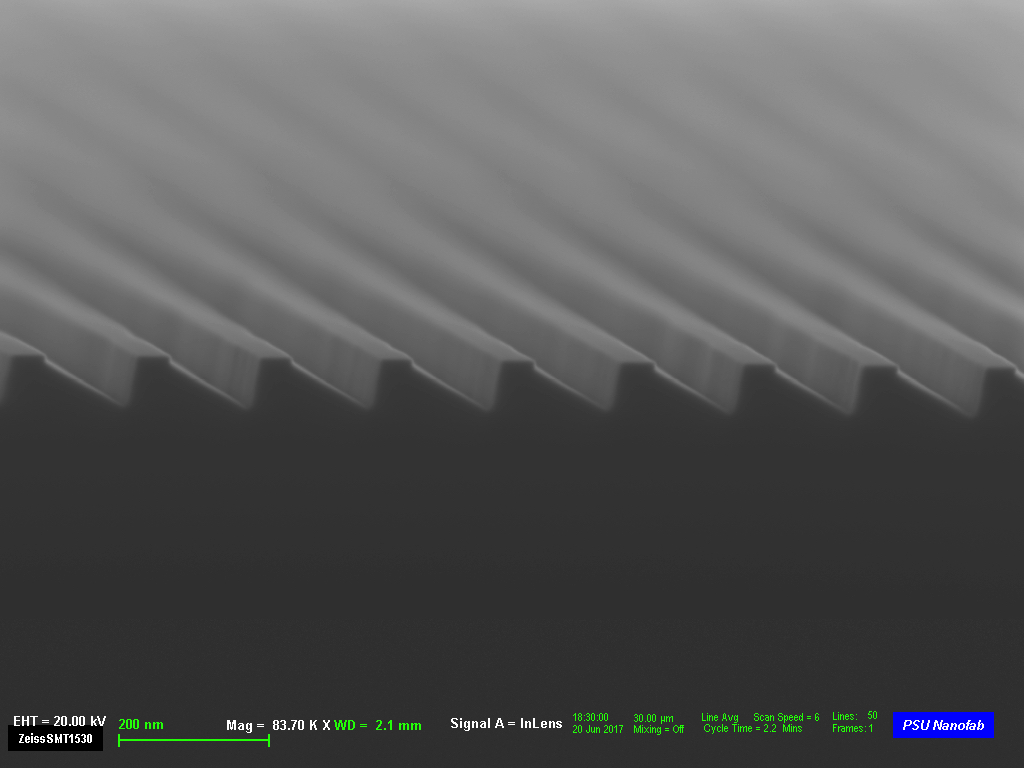
\includegraphics[scale=0.4]{Chapter-1/Figures/master_04.jpg}
 \caption[Field-emission scanning electron micrograph (FESEM) of a \ce{KOH}-etched grating viewed edge-on.]{Field-emission scanning electron micrograph (FESEM) of a \ce{KOH}-etched grating with $d \lessapprox \SI{160}{\nm}$ viewed edge-on, taken with a \textsc{Zeiss Leo 1530} instrument at the Penn State Nanofabrication Laboratory. Due to the $\langle 311 \rangle$ surface orientation of the silicon wafer used for processing, the etched sawtooth structure nominally features an active blaze angle of $\delta = 29.5^{\circ}$ and a steep-facet angle of $\bar{\delta} =  79.98^{\circ}$ [\emph{cf.\@} \cref{eq:311_angle,eq:311_angle2}]. Flat tops that protrude above the sawtooth pattern exist as a result of the \ce{Si_{x}N_{y}} etch mask [\emph{cf.\@} \cref{fig:master_fab}] while the groove depth follows from \cref{eq:groove_depth} \cite{McCoy17,Miles18,McCoy20b}.}\label{fig:master_grating_SEM}
 \end{figure}
This grating was fabricated by staff at the Penn State Nanofabrication Laboratory \cite{PSU_MRI_nanofab} in a process that used EBL to pattern a groove layout in resist, RIE to transfer the pattern into a \SI{30}{nm}-thick LPCVD layer of \ce{Si_{x}N_{y}} [\emph{cf.\@} footnotes~\ref{footnote:dry_etch_RIE} and \ref{footnote:nitride_mask}] and a timed, room-temperature \ce{KOH} etch to produce a sawtooth-like surface relief \cite{Miles18}. 
Following the procurement of a \SI{500}{\um}-thick, \SI{150}{\mm}-diameter silicon wafer from \textsc{Virginia Semiconductor} \cite{Virgsemi_web} with a $\langle 311 \rangle$ surface orientation and a pre-deposited, low-stress layer of \ce{Si_{x}N_{y}} \cite{Zheng13}, the groove layout was defined by EBL in a \SI{140}{\nm}-thick layer of ZEP520A resist, which was obtained by spin-coating a 1:1 mixture of the resist in Anisole (\emph{i.e.}, \emph{methoxybenzene}; \ce{C7H8O})\footnote{This was done at \num{3000} rotations per \si{\minute} for \SI{45}{\second} following a \SI{3}{\minute} dehydration hotplate bake at \SI{180}{\celsius}; the Anisole was then removed from the resist with an identical hotplate bake.} (\cref{fig:master_fab}, step 1). 
\begin{figure} 
 \centering
 \includegraphics[scale=1.08]{Chapter-1/Figures/master_fab1.mps}
 \includegraphics[scale=1.08]{Chapter-1/Figures/master_fab2.mps}
 \includegraphics[scale=1.08]{Chapter-1/Figures/master_fab3.mps}
 \includegraphics[scale=1.08]{Chapter-1/Figures/master_fab4.mps}
 \includegraphics[scale=1.08]{Chapter-1/Figures/master_fab5.mps}
 \includegraphics[scale=1.08]{Chapter-1/Figures/master_fab6.mps}
 \includegraphics[scale=1.08]{Chapter-1/Figures/master_fab7.mps}
 \includegraphics[scale=1.08]{Chapter-1/Figures/master_fab8.mps}
 \caption[Outline of fabrication recipe for crystallographic etching in a $\langle 311 \rangle$-oriented silicon wafer using EBL]{Outline of fabrication recipe for crystallographic etching in a $\langle 311 \rangle$-oriented silicon wafer using EBL. A wafer coated with \ce{Si_{x}N_{y}} is spin-coated with resist, where a groove layout is defined by EBL. This pattern is transferred into the \ce{Si_{x}N_{y}} and then the resist is removed through reactive ion etching (RIE). Native \ce{SiO2} on the wafer is removed with a buffered oxide etch (BOE) before a timed crystallographic etch using \ce{KOH} is carried out to expose $\{ 111 \}$ planes that intersect at an angle of $\theta = 70.53^{\circ}$. Finally, the \ce{Si_{x}N_{y}} is removed using \ce{HF}, leaving groove structure with a depth $h$ and flat-top width $w$ that both depend on $d$ and the degree of \ce{KOH}-etch undercut by \cref{eq:groove_depth} \cite{McCoy17,Miles18}.}\label{fig:master_fab} 
 \end{figure}
Using the \textsc{EBPG5200} tool at Penn State described in \cref{sec:binary_ebeam}, the resist was patterned over a variable-line-space profile \SI{75}{\mm} by \SI{96}{\mm} in area that approximates a radial profile [\emph{cf.\@} \cref{sec:grating_tech_intro}] with groove spacing $d \lessapprox \SI{160}{\nm}$ to match a \SI{12}{\metre} focal length.\footnote{This was baselined for a preliminary design of \emph{Arcus}, a proposed soft x-ray spectrometer \cite{Smith19_arcus,Arcus_web}.} 
The groove layout was designed as six sections of parallel lines, each with a different value of $d$, and then fractured from computer-aided design into data understandable to the \textsc{EBPG5200} using the \textsc{Layout BEAMER} software package.\footnote{With a \SI{0.25}{\nm} resolution for the \textsc{EBPG5200} and a \SI{40}{\nm} beam step size in \textsc{Layout BEAMER}, $d$ for each section of parallel grooves ranges nominally from \SIrange{160}{158.25}{\nm}, in steps of \SI{0.25}{\nm}.} 
These lines and spaces were exposed using a nominal electron dose of $D = \SI{170}{\micro\coulomb\per\cm\squared}$, a \SI{60}{\nano\ampere} beam current, a \SI{200}{\um} aperture size, and a \SI{40}{\nm} beam step size, to a duty cycle of $\sim \SI{50}{\percent}$ and then developed at room temperature in \emph{n-amyl acetate} (\ce{C7H14O2}) for \SI{3}{\minute} and IPA for \SI{30}{\second} followed by a high-purity nitrogen blow dry (\cref{fig:master_fab}, step 2). 
\begin{figure}
 \centering
 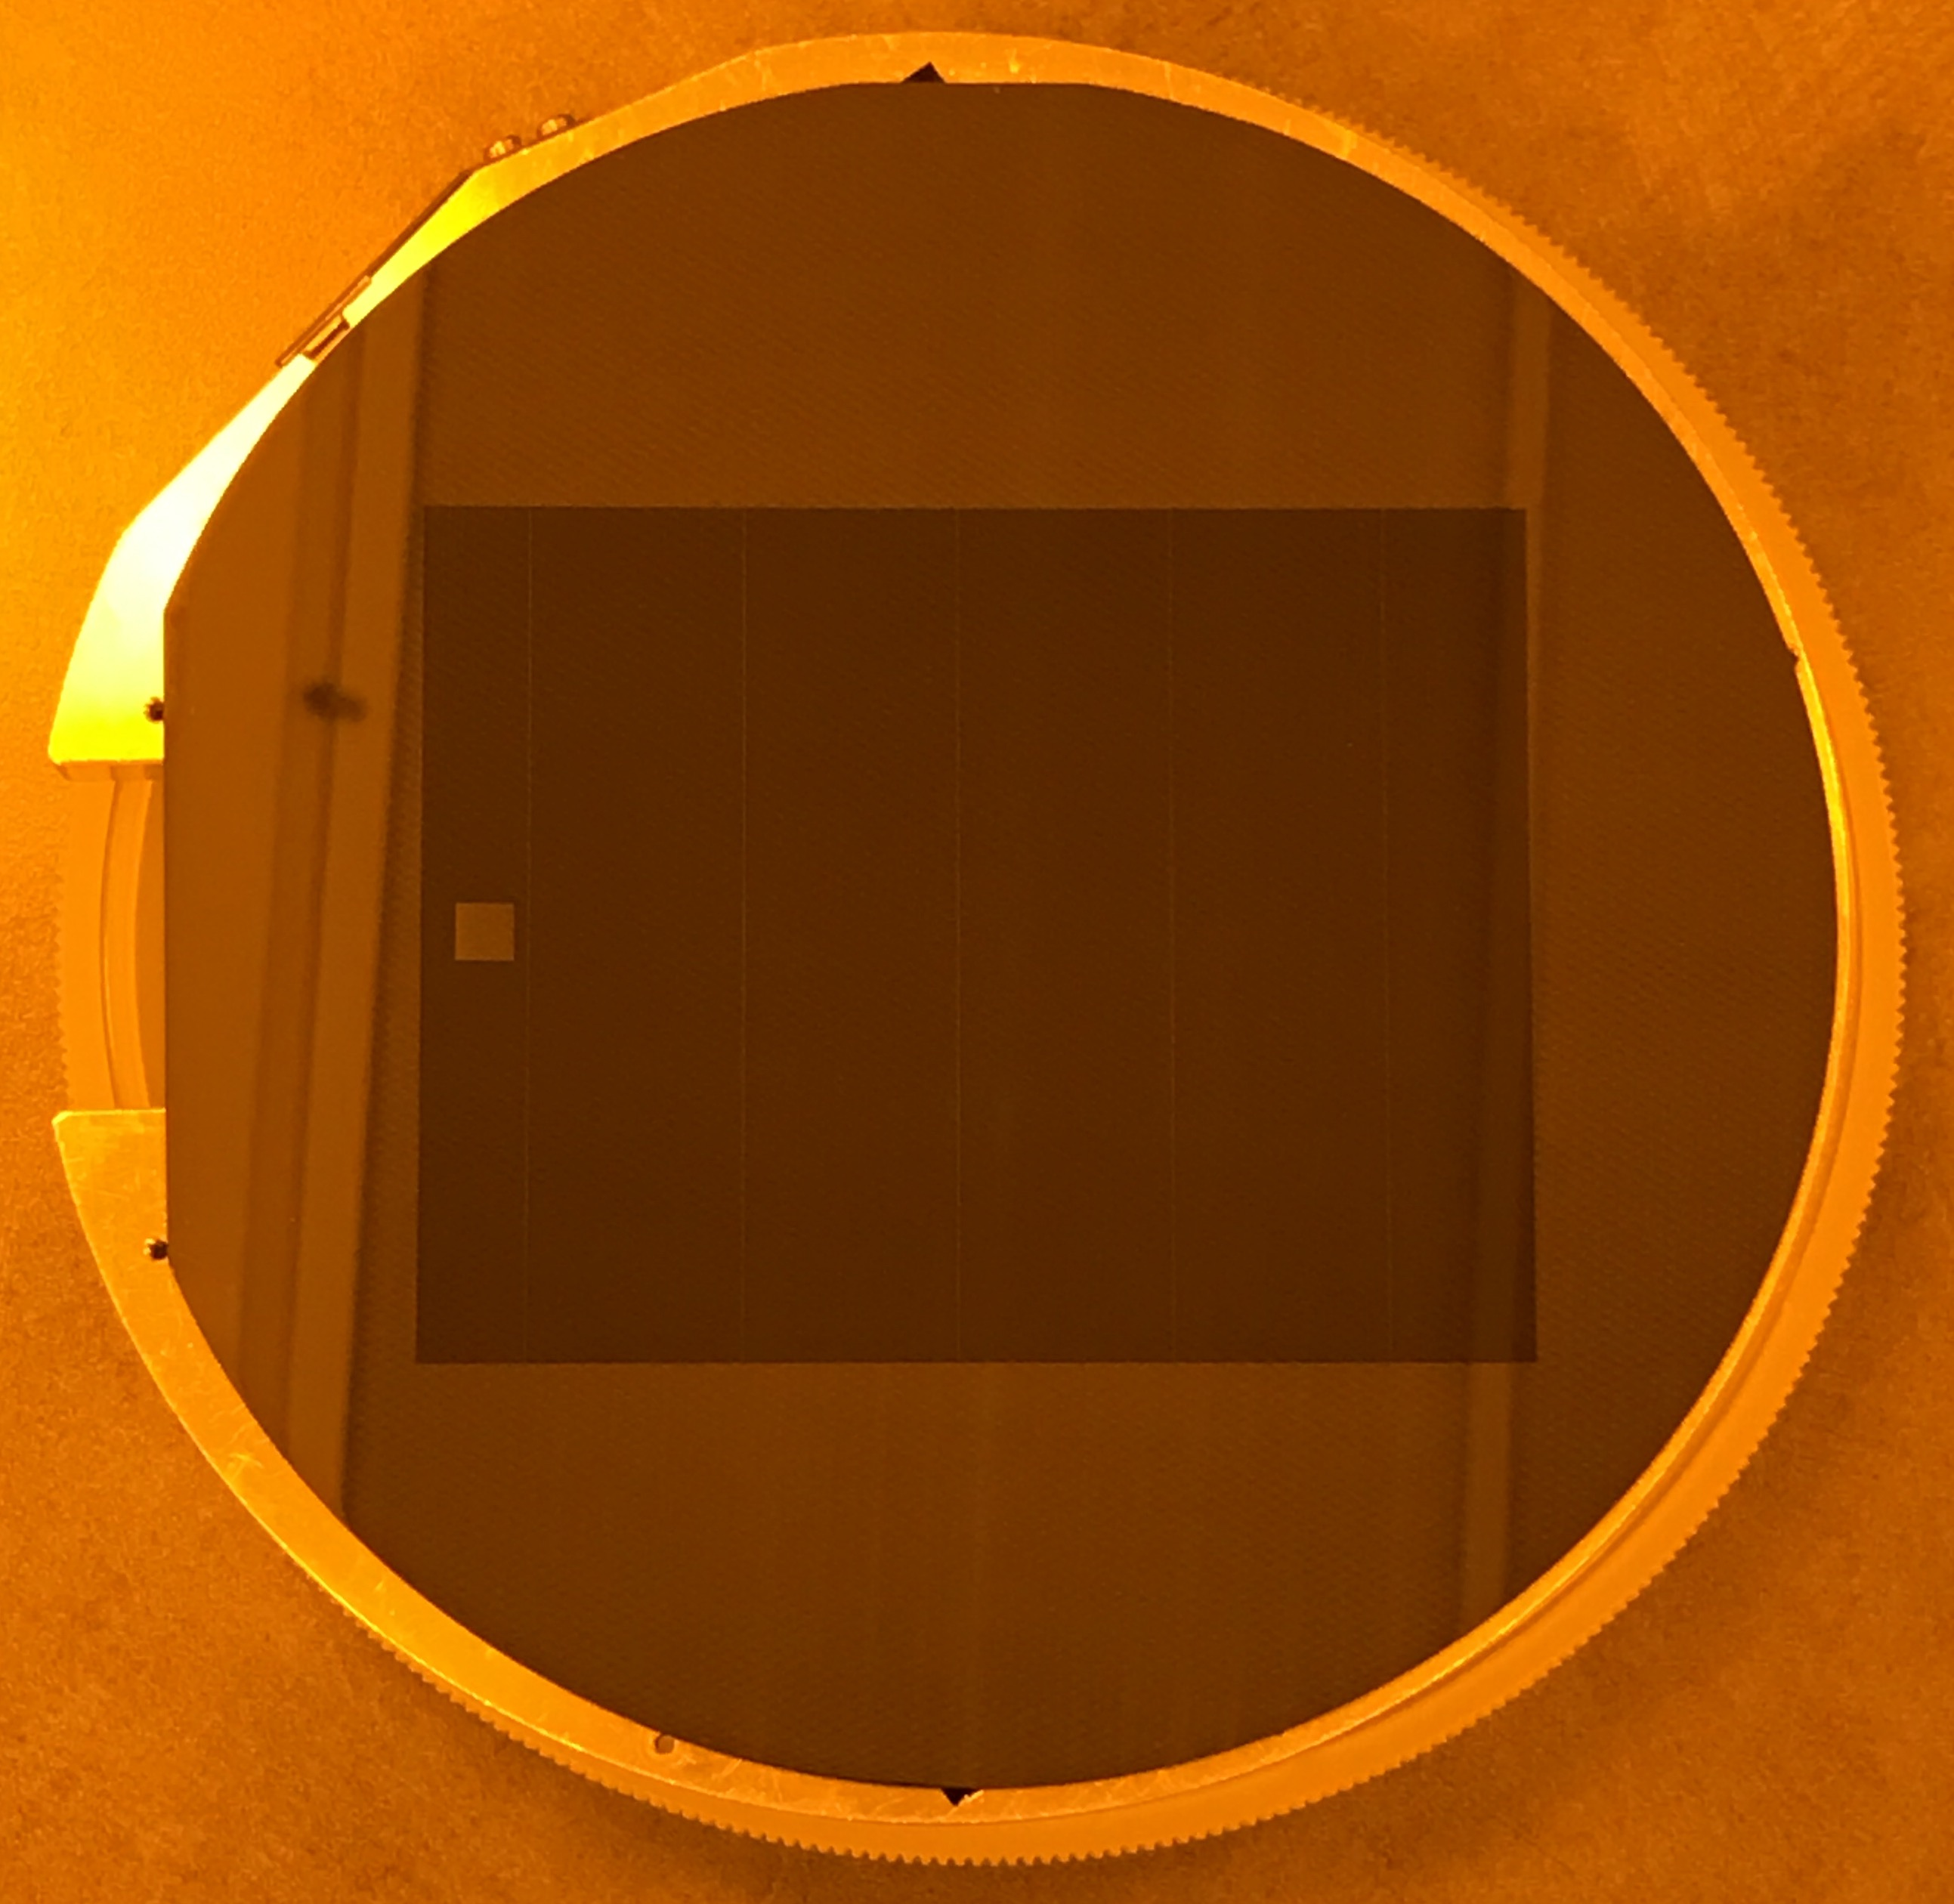
\includegraphics[scale=0.15]{Chapter-1/Figures/master_grating.jpg}
 \caption[\ce{KOH}-etched grating patterned over a \SI{75}{\mm} by \SI{96}{\mm} area on a \SI{150}{\mm}-diameter, $\langle 311 \rangle$-oriented wafer.]{Photograph of the \SI{75}{\mm} by \SI{96}{\mm} grating depicted in \cref{fig:master_grating_SEM}, shown patterned on a \SI{150}{\mm}-dimater, $\langle 311 \rangle$-oriented wafer with grooves oriented horizontally. Also seen are thin lines of unpatterned area in between each section of parallel grooves and a small, square optical grating used for aligning off-plane gratings in a module \cite{McCoy17}.}\label{fig:master_grating} %\cite{Miles18}
 \end{figure}

The EBL-patterned resist was transferred into the underlying \ce{Si_{x}N_{y}} film through RIE processing carried out with a \textsc{Plasma-Therm Versalock} tool, which consisted of a short descum with an oxygen (\ce{O2}) plasma to remove residual exposed resist followed by plasma etch using a mixture of \emph{fluoroform} (\ce{CHF3}) and \ce{O2} (\cref{fig:master_fab}, step 3a). 
To prepare for the crystallographic etch, remaining resist was removed by oxidation with another \ce{O2} RIE (\cref{fig:master_fab}, step 3b) before a BOE [\emph{cf.\@} footnote~\ref{footnote:buffered_oxide_etch}] was carried out to remove native \ce{SiO2} on the wafer surface (\cref{fig:master_fab}, step 4). 
The wet anisotropic etch was performed in \SI{45}{\percent}-diluted \ce{KOH} at room temperature for \SI{24}{\min} to produce an asymmetric sawtooth with a narrow flat top beneath the \ce{Si_{x}N_{y}} mask and a sharp point at the bottom of each groove (\cref{fig:master_fab}, steps 5a and 5b). 
Finally, the \ce{Si_{x}N_{y}} mask was stripped with a \SI{10}{\min} etch in \SI{49}{\percent}-diluted \ce{HF} (\cref{fig:master_fab}, step 6), leaving the structure of a surface-relief grating with a nominal blaze angle of $\delta = 29.5^\circ$ and a top plateau of width $w \gtrapprox \SI{30}{\nm}$ so that the groove depth is given by 
\begin{equation}\label{eq:groove_depth}
 h \approx \frac{d - w}{\cot \left( \delta \right) - \cot \left( \theta + \delta \right)} + \Delta h ,
 \end{equation}
where $\Delta h$ is the vertical protrusion of the top plateau \cite{McCoy20b}. 
While these sharp grooves prevent $h$ to be measured by AFM without a high-aspect-ratio scanning probe tip, it is estimated that this quantity falls within the range \SIrange{65}{70}{\nm} with $\Delta h$ of a few \si{\nm}. 
The \SI{72}{\cm\squared} patterned area following all fabrication steps is shown on a \SI{150}{\mm}-diameter wafer in \cref{fig:master_grating}. 

Grating fabrication processes centering on \ce{KOH} etching are beneficial especially for producing sawtooth-like structures with exceptionally smooth facets at a specified blaze angle that depends on the crystallographic orientation of the wafer used for processing \cite{Franke97,McEntaffer13,DeRoo16thesis}. 
While these high-fidelity structures lend themselves to high overall diffraction efficiency and an effective blaze response, ideally the topography would be inverted to achieve a sharp groove apex with the flat tops produced by the \ce{Si_{x}N_{y}} etch mask laying at the groove base, which is usually shadowed by incident radiation. 
This can be achieved through grating replication via nanoimprint lithography \cite[\emph{cf.\@} \cref{sec:nanoimprint}]{Chang03} but there are still important disadvantages that come along with fabricating a master grating in this way. %through \ce{KOH} etching. 
First, \ce{KOH} etching demands precise alignment between the groove direction and the appropriate crystallographic axis (\emph{i.e.}, $\langle 011 \rangle$ in most cases) to achieve smooth and continuous groove facets. 
Moreover, the face-centered cubic structure of silicon [\emph{cf.\@} \cref{fig:crystal_structure}] ultimately prevents the formation of a true radial profile even with a hypothetically perfect alignment. 
In a \ce{KOH}-etched $\langle 311 \rangle$-oriented wafer, for example, the distance between $\{ 111 \}$ planes, $d_{111} \equiv a_{\text{Si}}/\sqrt{3}$, projects to a lateral spacing on the surface of the wafer of 
\begin{equation}
 \Delta d \equiv d_{111} \sin \left( \delta \right) \approx \SI{0.15}{\nm} \quad \text{for } \delta = 29.5^{\circ} . 
 \end{equation}
A radial profile patterned in a resist film by EBL, therefore, would still result in the formation of groove facets that are confined to this quantized groove spacing imposed by the crystal structure and, in principle, slight misalignments with the crystallographic planes combined with this latter issue lead to $\mathscr{R}$ being degraded in a Wolter-I grating spectrometer. 
Although this has yet to be confirmed by published testing results, it is worthwhile to investigate alternative nanofabrication techniques that enable a high-precision radial profile to be preserved while also achieving blazed groove facets to maximize spectral sensitivity in a given bandpass of interest. 

\subsubsection{Nanoimprint Lithography for Grating Replication}\label{sec:nanoimprint}
%%%%%%%%%%%%%%%%%%%%%%%%%%%%%%%%%%%%%%%%%--------------------------------------------------
The nanofabrication methods described in \cref{sec:holographic,sec:binary_ebeam,sec:crystal_etching} are suitable for a variety of custom reflection gratings but due to their complexity and potentially long manufacturing times, it is typically not practical to produce a large number of gratings for a Wolter-I spectrometer by using these processes to fabricate each grating directly. 
Reflection gratings fabricated by mechanical ruling engine are commonly replicated using processes where a suitable synthetic resin, such as epoxy, takes on the inverse mold of the master grating \cite{Loewen97,Franke97}.  
This resin is dispensed on the master grating and then a blank substrate is brought into contact while the material cures; a replica is produced on the blank substrate following separation of the mold and the master grating. 
Such processes, however, usually produce relatively low-fidelity replicas and become increasingly difficult for gratings with sub-\si{\um} groove period. 
Nonetheless, the surface-relief molds of the \num{182} gratings used for the \emph{RGS} on board \emph{XMM-Newton} were manufactured in this way before each was coated in gold for soft x-ray reflectivity \cite{Kahn96,denHerder01}. 

\emph{Nanoimprint lithography (NIL)} describes a class of nanofabrication techniques first developed in the mid 1990s as a method for high-throughput manufacturing of devices featuring nanoscale structures \cite{Chou96,Haisma96,Schift08,Schift10}. 
These techniques are resist-based similar to EBL [\emph{cf.\@} \cref{sec:binary_ebeam}] but rather than using radiation or particle exposure followed by wet development, the method of patterning is by molding through direct contact between a stamp (\emph{e.g.}, a master grating) and a layer of resist coated on a blank substrate. 
Moreover, the resist must be in a state where it is able to flow like a liquid with relatively low viscosity for the material to be able to mold to the inverse of the stamp. 
This typically occurs in polymers $\gtrapprox \SI{50}{\celsius}$ above their \emph{glass transition temperature}, $T_g$, which marks the smooth transition from a solid to a liquid in an amorphous material, which is in contrast to the thermodynamics of melting in a crystalline structure that involves latent heat \cite{Schift10,Kirchner19,Trolier-McKinstry17}. 

In the original variant of NIL, known as \emph{thermal NIL} or a type of \emph{hot embossing}, the resist can be heated to a temperature well above $T_g$ so that it is able to fill the stamp features with applied pressure on a specialized imprint tool \cite{Chou96,Schift10}. 
Then, by bringing the temperature back down below $T_g$, the stamp can be de-molded from the resist, leaving the imprinted pattern. 
\begin{figure}
 \centering
 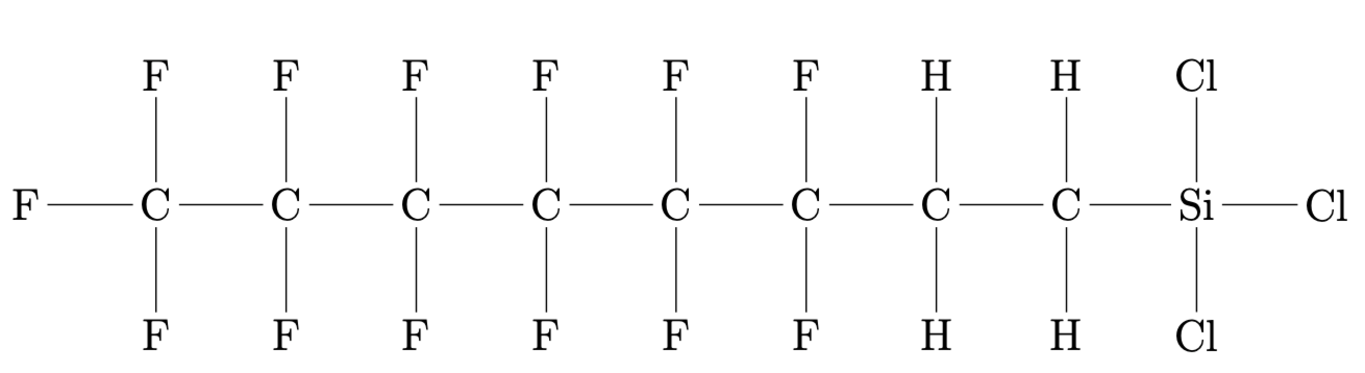
\includegraphics[scale=0.65]{Chapter-1/Figures/FOTS.pdf}
 \caption[Structural formula of perfluorooctyltrichlorosilane (FOTS).]{Structural formula of FOTS with a \ce{-SiCl3} active head group and a \ce{-CF3} surface terminal group. Along with other similar materials, a self-assembled monolayer of FOTS can be used as an anti-adhesive layer in NIL for stamps with silicon surfaces.}\label{fig:FOTS}
 \end{figure}
However, this process must be carried out carefully to avoid degradation of the stamp and additionally, an anti-adhesive coating on the stamp is often required to prevent the imprint resist from sticking to the stamp. 
For a silicon surface with native oxide, this can be accomplished with a fluorinated trichlorosilane such as \emph{perfluorooctyltrichlorosilane} (FOTS; \ce{C8H4Cl3F13Si}) or \emph{perfluorodecyltrichlorosilane} (FDTS; \ce{C10H4Cl3F17Si}) \cite{Schift10,Zhuang07}.\footnote{Note, however, that different types of chemicals are required for other surfaces (\emph{e.g.}, gold \cite{Kim_2002}).} 
Such a material can be coated by \emph{molecular vapor deposition} on a hydroxylated silicon surface\footnote{\emph{i.e.}, such that hydroxyl groups (\ce{-OH}) are bonded to the native \ce{SiO2}} \cite{Kobrin05,Zhuang07,Verschuuren10}.
This process works by injecting the chosen chemical along with water vapor (\ce{H2O}) into a vacuum chamber so that the \ce{-SiCl3} active head groups on the molecule [\emph{cf.\@} \cref{fig:FOTS}] react with \ce{H2O} as well as \ce{SiO2} on the surface of the stamp. 
The sites on the molecule normally occupied by chlorine are in this case replaced by hydroxyl groups from the vapor as well as oxygen present in the native oxide. 
With \emph{hydrochloric acid} (\ce{HCl}) and \ce{H2O} as by-products, this bonds the fluorinated trichlorosilane to the stamp surface as a \emph{self-assembled monolayer} so that it becomes chemically inert and hydrophobic, thereby preventing adhesion with the imprint resist \cite{Zhuang05,Zhuang07,Schift10}. 

The first resist to be used for NIL was PMMA \cite{Chou96}, which was introduced in the context of EBL in \cref{sec:binary_ebeam} with its structural chemical composition shown in \cref{fig:PMMA}. 
While EBL typically calls for PMMA with relatively high $M_w$ (\emph{e.g.}, \SI{950}{\kilogram\per\mole}), PMMA used for NIL commonly has $M_w$ on the order of tens of \si{\kilogram\per\mole} so that with its thermoplastic properties, the material has decreased viscosity at temperatures above $T_g$, that correlate with $M_w$ below a critical value, $M_c$, which depends on various properties of the synthesized polymer \cite{Fuchs96,Geng16,Schift10,Kirchner19}. 
Although a low $M_w$ allows the molecules to fill small stamp features more easily, the resist is in a relatively soft state at room temperature due to $M_w$ being comparable to $M_c \approx \SI{10}{\kilogram\per\mole}$ for PMMA \cite{Schift10,Schleunitz10,Kirchner19}. 
This practically prevents the imprinted pattern from being used as a functional material and instead limits it to be used as an etch mask under appropriate conditions. 

NIL can also be used with UV-curable resists in a variant of the process known as \emph{UV-NIL} \cite{Haisma96}, where the resist is in a liquid state at room temperature so that the material can flow into the features of the applied stamp. 
This liquid-state material then is cross-linked by UV radiation, which serves to increase $M_w$ as well as $T_g$ so that the imprinted pattern becomes solidified at room temperature \cite{Schift08,Schift10}. 
With the resist being cured by UV radiation, its mechanical stability is improved so that the imprinted pattern can be used as a more functional structure for a reflection grating. 
However, the curing of the resist also changes the polymer structure of the material through cross-linking and hence some degree of volumetric shrinkage is expected in the imprinted pattern \cite{Horiba_2012}. 
While this effect may be small depending on the nature of the material, this shrinkage can, in principle, lead to imprinted gratings with a blaze angle $\delta'$ that is reduced relative to that of the master grating, $\delta$. 
Therefore, this effect of $\delta' < \delta$ generally must be accounted for to ensure that diffraction efficiency is maximized in the intended spectral bandpass [\emph{cf.\@} \cref{sec:discussion_scil}]. 

UV-NIL has been pursued previously to replicate gratings from master templates fabricated using the crystallographic etching technique described in \cref{sec:crystal_etching} \cite{Chang03,Chang04,McEntaffer13,DeRoo16thesis,DeRoo16,Miles18}. 
\begin{figure} 
 \centering
 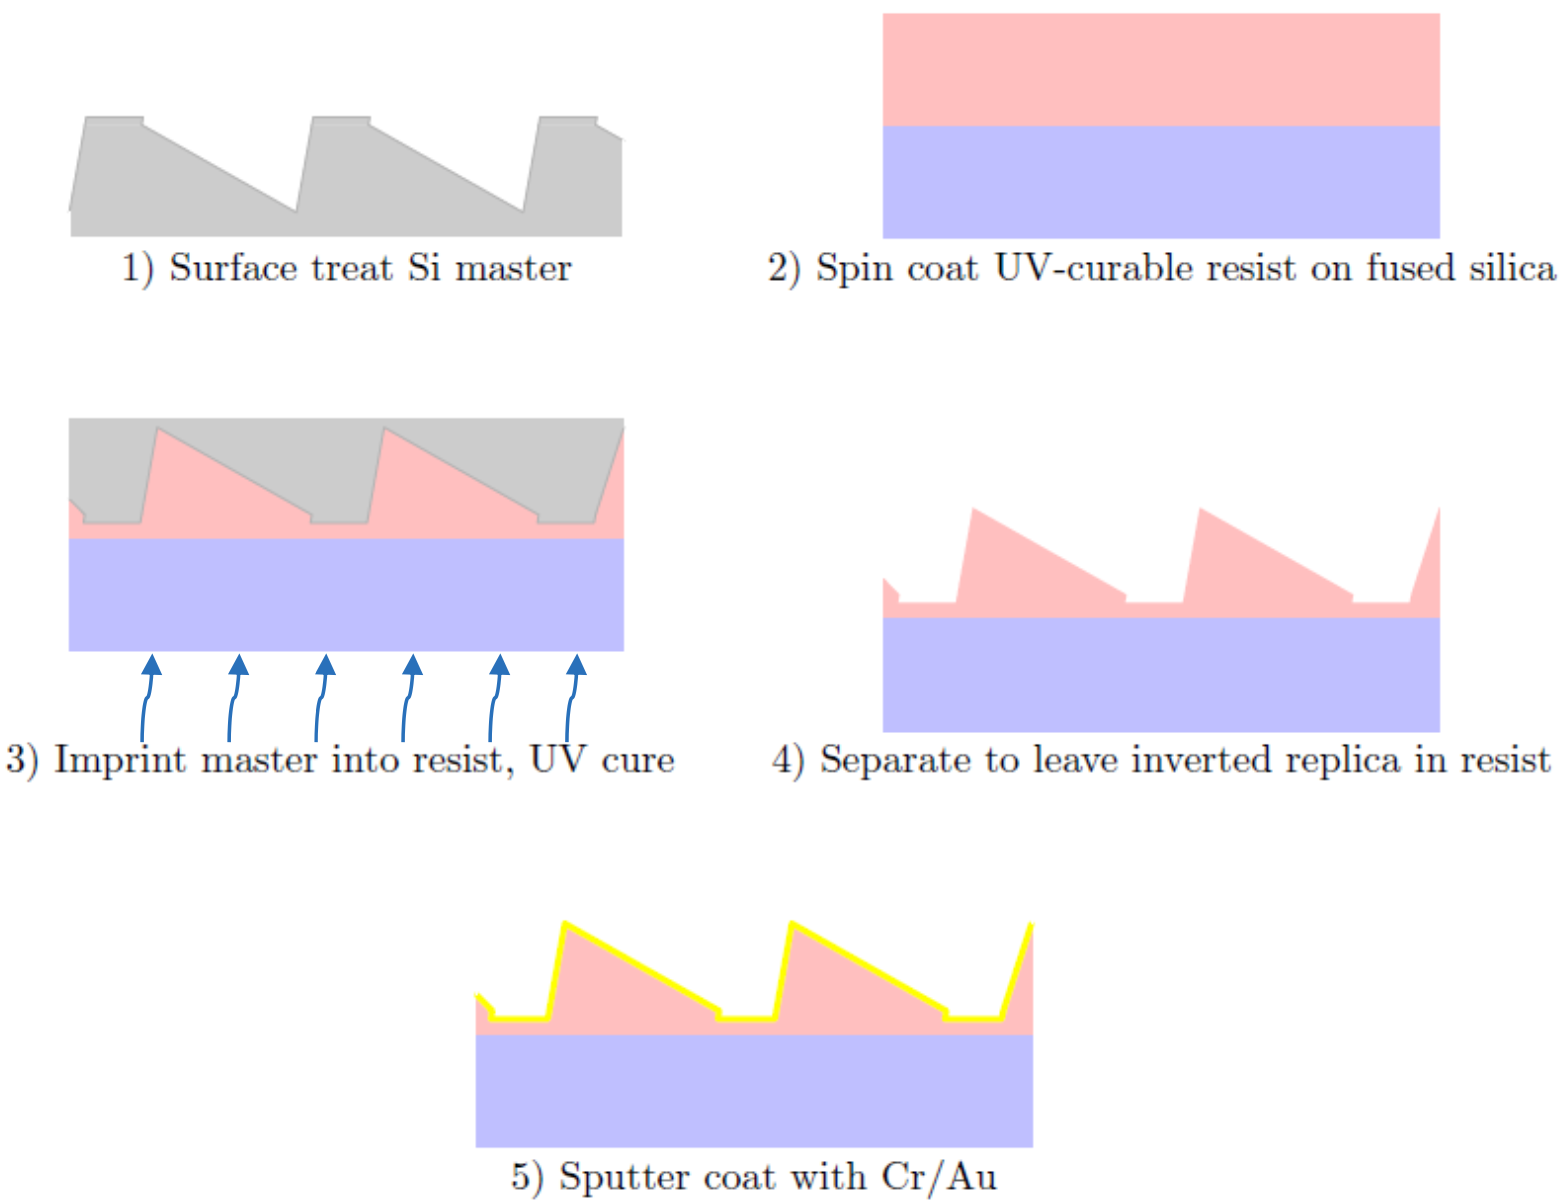
\includegraphics[scale=0.55]{Chapter-1/Figures/UV-NIL.PNG}
 \caption[Outline of a grating replication process that uses a \ce{KOH}-etched master grating to imprint to ultraviolet-curable resist by UV-NIL.]{Outline of a grating replication process that used UV-NIL to imprint a \ce{KOH}-etched master grating into UV-curable resist \cite{Miles18}.}\label{fig:uv_nil} 
 \end{figure}
This process is illustrated in \cref{fig:uv_nil} for a grating fabrication scheme that used the \ce{KOH}-etched, $\langle 311 \rangle$-oriented wafer depicted in \cref{fig:master_grating_SEM,fig:master_fab,fig:master_grating} as a \SI{72}{\cm\squared} master grating; imprinting was carried out by \textsc{Nanonex Corporation} \cite{nanonex} using their \textsc{NX-2000} imprint tool and proprietary materials for the anti-adhesive layer (\textsc{NXT-130}), the imprint resist (\textsc{NXR-2050}), as well as an adhesion promoter (\textsc{NXT-404}) for the resist and a blank substrate \cite{Miles18}. 
While UV-NIL is commonly carried out using a stamp that is transparent to UV radiation (\emph{e.g.}, quartz) and a blank (opaque) silicon substrate \cite{Schift10}, the master grating in this case is made of silicon, which led to the need for an UV-transparent imprint wafer. 
Therefore, following the surface treatment for anti-stiction using \textsc{NXT-130} (\cref{fig:uv_nil}, step 1), a layer of \textsc{NXR-2050} resist was spin-coated on a \SI{150}{\mm}-diameter, fused-silica substrate, using \textsc{NXT-404} as an adhesion promoter (\cref{fig:uv_nil}, step 2). 
Based on the \SIrange{65}{70}{\nm} groove depth of the master grating [\emph{cf.\@} \cref{sec:crystal_etching}] this layer of resist was coated as a \SI{200}{\nm}-thick film so that the liquid resist could fill the features of the stamp adequately. 

Using an \textsc{NX-2000} imprinting tool, the master grating was then brought into contact with the coated substrate so that the \textsc{NXR-2050} resist could mold to the inverse of the stamp. 
The resist was then cured by exposing it to UV radiation through the fused-silica substrate (\cref{fig:uv_nil}, step 3) before the stamp was separated from the imprinted pattern (\cref{fig:uv_nil}, step 4). 
\begin{figure} 
 \centering
 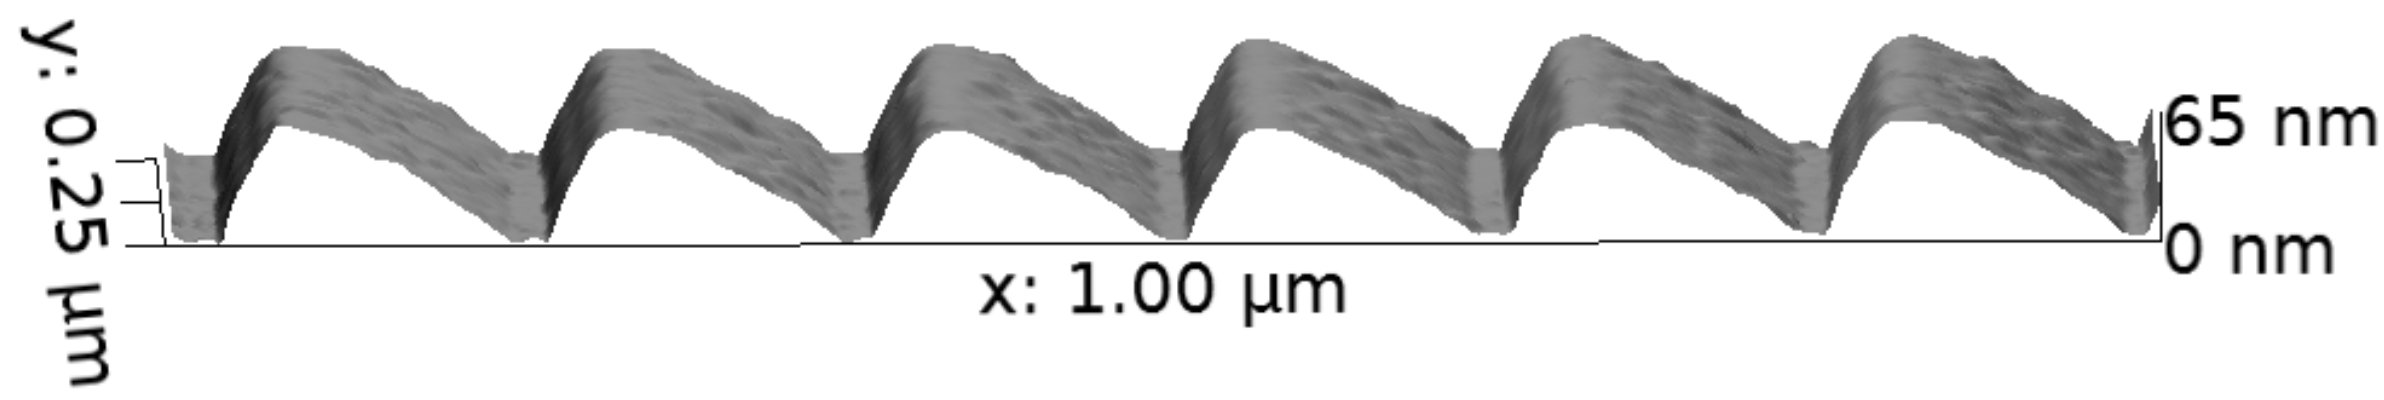
\includegraphics[scale=0.37]{Chapter-1/Figures/UV-NIL_AFM.PNG}
 \caption[AFM of a blazed grating fabricated by UV-NIL from a \ce{KOH}-etched master (credit: T.\ Tighe)]{AFM of a blazed grating fabricated by UV-NIL from a \ce{KOH}-etched master. Image credit: T.\ Tighe at the Penn State MCL \cite{Miles18}.}\label{fig:uv_nil_AFM} 
 \end{figure}
Finally, the patterned resist featuring the inverse topography of the master was coated with a $\sim \SI{15}{\nm}$-thick layer of gold for soft x-ray reflectivity using a $\sim \SI{5}{\nm}$-thick layer of chromium for adhesion,\footnote{The reasoning for the use of the materials is discussed in \cref{sec:total_refl}.} which was accomplished via \emph{plasma sputter deposition} by staff at the Penn State Nanofabrication Laboratory \cite{PSU_MRI_nanofab} using a \textsc{Kurt J.\ Lesker CMS-18} tool \cite{Miles18}. 
This final, coated imprint is shown under AFM in \cref{fig:uv_nil_AFM}.\footnote{Credit for AFM is owed to T.\ Tighe at the Penn State MCL \cite{PSU_MRI_CL,Miles18}.}. 

Although NIL is a proven technology for replicating nanoscale patterns in a variety of applications, there are aspects of this process that lead to difficulties for x-ray reflection gratings. 
First, the rigidity of a silicon stamp requires a relatively high pressure to be applied for imprints of substantial area (\emph{e.g.}, the \SI{72}{\cm\squared} silicon master described above) so that conformal contact between the stamp and the resist-coated blank substrate can be achieved and air pockets can be avoided \cite{Schift08,Schift10}. 
These conditions also lead to imprinting imperfections arising from particulate contaminants that may be present in the laboratory environment and, potentially, damage to the stamp surface. 
Additionally, a rigid stamp is gradually degraded as it makes repeated imprints. 
For example, in the case of the \textsc{Nanonex} UV-NIL process just described \cite{Miles18}, a single stamp typically can produce tens of quality replicas \cite{Schift08,Schift10}. 
With the \emph{XGS} for \emph{Lynx} calling for thousands of replicated gratings \cite{McEntaffer19}, however, this becomes impractical especially for large, expensive silicon masters that are fabricated using EBL. 
Therefore, an alternative, high-throughput grating replication technique is needed to identify a process capable of meeting this manufacturing requirement. 

\section{Conclusions and Outline of This Thesis}\label{sec:ch1_conclusions}
%%%%%%%%%%%%%%%%%%%%%%%%%%%%%%%%%%%%%%%%%--------------------------------------------------
Measuring the diffuse, highly-ionized baryonic content in the extended halos of isolated galaxies, groups or clusters, and the warm-hot intergalactic medium through soft x-ray absorption spectroscopy of active galactic nuclei is a main scientific objective for the currently-planned \emph{Lynx X-ray Observatory} \cite[\emph{cf.\@} \cref{sec:astro_plasmas}]{Lynx_web,Gaskin19}. 
These observations demand high spectral sensitivity coupled with high spectral resolving power, $\mathscr{R}$, to enable faint absorption lines to be distinguished from continua at a level that offers a significant improvement over the capabilities of current instruments on board the spacecraft observatories \emph{Chandra} and \emph{XMM-Newton}. 
While microcalorimeters satisfy this need for many other areas of x-ray spectroscopy, a state-of-the-art grating spectrometer with a large effective collecting area is better suited for measuring faint absorption lines from abundant highly-charged ions that fall in the soft x-ray bandpass. 
The specialized x-ray reflection gratings described in \cref{sec:grating_tech_dev} are one of two technologies considered for the \emph{Lynx XGS} \cite{McEntaffer19}, with the other being critical-angle transmission gratings \cite{Heilmann11,Heilmann16,Gunther19}.
From the standpoint of grating fabrication, the main technological challenges are: 
\begin{enumerate}[noitemsep]
    \item producing a master grating with a sawtooth surface-relief profile that enables 
    \begin{enumerate}[noitemsep]
        \item total absolute diffraction efficiency in the soft x-ray exceeding \SI{40}{\percent}, and 
        \item $\mathscr{R} \gtrapprox 5000$ in a Wolter-I telescope
    \end{enumerate}
    and additionally,  
    \item mass-replicating blazed gratings to populate modular grating arrays for a soft x-ray spectrometer such as the \emph{XGS}. 
\end{enumerate}
This dissertation contributes to these two areas of reflection grating research with an emphasis on applied nanofabrication and beamline diffraction-efficiency testing. 
Mentioned at the start of this chapter, the focus in particular is on the implementation of two recently-developed techniques in nanofabrication that are hypothesized to be capable of meeting these goals and their subsequent testing for diffraction efficiency at beamline 6.3.2 of the Advanced Light Source \cite{ALS_web,ALS_632,Underwood96,Gullikson01}; beamline testing for spectral resolving power is beyond the scope of this dissertation. 

First, \cref{ch:master_fab} introduces the process of \emph{thermally-activated selective topography equilibration (TASTE)} \cite{Schleunitz14}, which utilizes \emph{grayscale electron-beam lithography} and \emph{polymer reflow} [\emph{cf.\@} \cref{sec:TASTE}] to generate smooth and continuous reliefs in a thermoplastic resist, as a means for fabricating a master grating. %sec:TASTE
This technique has the key advantage that blazed groove facets can, in principle, be patterned over a radial groove layout without dependence on crystallographic structure that can lead to a degradation in $\mathscr{R}$ as alluded to in \cref{sec:crystal_etching}. 
While \si{\um}-scale sawtooth structures fabricated by TASTE have been reported on in the literature \cite{Schleunitz10,Schleunitz14,Kirchner16,Kirchner19}, applying this process to x-ray reflection grating technology requires the realization of a blazed-grating surface relief with a groove spacing of a few hundred \si{\nm} that performs with high diffraction efficiency in an extreme off-plane mount when coated with an appropriate metal for reflectivity. 
As described in \cref{ch:master_fab}, this is carried out through the development of a new fabrication recipe for TASTE at the Penn State Nanofabrication Laboratory \cite{PSU_MRI_nanofab} and the implementation of this process for fabricating a blazed-grating prototype with parallel grooves that is suitable for diffraction-efficiency testing \cite{McCoy18,McCoy20}. 
These results serve as proof of concept for x-ray reflection grating fabrication by TASTE and a basis for future experiments that will examine the ability of this process to pattern a radial groove profile that enables high $\mathscr{R}$ in a Wolter-I spectrometer. 

The second subject of this dissertation, which is addressed in \cref{ch:grating_replication}, is on \emph{substrate-conformal imprint lithography (SCIL)} \cite{Verschuuren10,Verschuuren17} as a method for high-throughput grating replication. 
Developed by \textsc{Philips SCIL Nanoimprint Solutions} \cite{philis_scil}, this variant of NIL uses a flexible composite stamp formed from a rigid master template to pattern nanoscale features in an inorganic resist that cures thermodynamically through a silica \emph{sol-gel process}, which differs fundamentally from the behavior of the organic resists described in \cref{sec:nanoimprint}. %
Although SCIL enables the production of several hundred imprints before stamp degradation and avoids many of the detriments associated with large-area imprinting, the sol-gel resist suffers shrinkage dependent on the post-imprint cure temperature.  
To characterize this effect, \cref{ch:grating_replication} describes processing carried out by \textsc{Philips SCIL Nanoimprint Solutions} that uses the \ce{KOH}-etched silicon grating from \cref{sec:crystal_etching} as a master template for producing replicas similar to those fabricated by UV-NIL. 
The diffraction-efficiency performance of such a replica is then compared to that of the silicon master to show that sol-gel resist shrinkage induced by a low-temperature cure is responsible for an effective decrease in blaze wavelength, $\lambda_b$, that results from a facet angle reduction of a few degrees \cite{McCoy20b}. 
Leveraging from the first application of SCIL to x-ray reflection grating technology for the \emph{Water Recovery X-ray Rocket (WRXR)} \cite{Miles17,Miles18b,Miles19,Verschuuren18,Tutt19}, this research serves to inform grating production for future instruments such as \emph{The Rockets for Extended-source X-ray Spectroscopy (tREXS)} \cite{Miles19b,Tutt19b} and \emph{The Off-plane Grating Rocket Experiment (OGRE)} \cite{DeRoo13,McEntaffer14,DeRoo16thesis,Donovan18b,Tutt18,Donovan19a,Donovan19b}, in addition to the \emph{XGS} planned for \emph{Lynx} \cite{McEntaffer19} and other similar instruments, such as \emph{Arcus} \cite{Smith19_arcus,Arcus_web}. 
Conclusions and future outlook for this thesis are provided in \cref{ch:conclusions}.

%\emph{Arcus}, a proposed soft x-ray spectrometer \cite{Smith19_arcus}
